\documentclass{report}

\usepackage[T1]{fontenc}
\usepackage[utf8]{inputenc}
\usepackage{times}

\usepackage[font=small,labelfont=bf,tableposition=top]{caption}
\usepackage{graphicx}
\usepackage{natbib} 

\usepackage{amsmath}
\usepackage{amsfonts}
\usepackage{amssymb}
\usepackage{color, soul}
\usepackage{hyperref}
\usepackage{algorithmicx}
\usepackage{algpseudocode}
\usepackage{subfigure}
\usepackage{stmaryrd}

\renewcommand{\vec}[1]{\boldsymbol{{#1}}} 
\newcommand{\duesoon}[1]{{\sethlcolor{green}\hl{#1}}}
\usepackage{mathrsfs}


\newtheorem{theorem}{Theorem}
\newtheorem{acknowledgement}[theorem]{Acknowledgement}
\newtheorem{algorithm}[theorem]{Algorithm}
\newtheorem{axiom}[theorem]{Axiom}
\newtheorem{case}[theorem]{Case}
\newtheorem{claim}[theorem]{Claim}
\newtheorem{conclusion}[theorem]{Conclusion}
\newtheorem{condition}[theorem]{Condition}
\newtheorem{conjecture}[theorem]{Conjecture}
\newtheorem{corollary}[theorem]{Corollary}
\newtheorem{criterion}[theorem]{Criterion}
\newtheorem{definition}[theorem]{Definition}
\newtheorem{example}[theorem]{Example}
\newtheorem{exercise}[theorem]{Exercise}
\newtheorem{lemma}[theorem]{Lemma}
\newtheorem{notation}[theorem]{Notation}
\newtheorem{problem}[theorem]{Problem}
\newtheorem{proposition}[theorem]{Proposition}
\newtheorem{remark}[theorem]{Remark}
\newtheorem{solution}[theorem]{Solution}
\newtheorem{summary}[theorem]{Summary}
\newenvironment{proof}[1][Proof]{\textbf{#1.} }{\ \rule{0.5em}{0.5em}}

\newtheorem{guess}{Definition}
\newcommand{\comment}[1] {}
\newcommand{\Norder} {N}
\newcommand{\order}{\mathcal{O}}
\newcommand{\Npoints} {N_p}
\newcommand{\Nfaces} {N_{f}}
\newcommand{\Nelements} {N_e}

\newcommand{\eps}{\varepsilon}
\newcommand{\Dweak}{\wt{D}}
\newcommand{\diff}[2] {\frac{\partial #1}{\partial #2}}
\newcommand{\dxx}[2] {\frac{\partial^2 #1}{\partial {#2}^2}}
\newcommand{\difft}[2] {\frac{d #1}{d #2}}
\newcommand{\dxxt}[2] {\frac{d^2 #1}{d {#2}^2}}
\newcommand{\lagrange}[1] {\frac{d #1}{dt}}
\newcommand{\lebesgue}{\parallel I \parallel}
\newcommand{\polysp}{\mathcal{P}_N}
\newcommand{\laplacian}{\nabla^2}
\newcommand{\divergence}{\nabla \cdot}
\newcommand{\inte}{\int_{\mbox{\footnotesize ${\Omega_e}$}}}
\newcommand{\intb}{\int_{\mbox{\footnotesize ${\Gamma_e}$}}}
\newcommand{\intce}{\int_{\mbox{\footnotesize ${\widehat{\Omega}_e}$}}}
\newcommand{\intcb}{\int_{\mbox{\footnotesize ${\widehat{\Gamma}_e}$}}}
\newcommand{\intg}{\int_{\mbox{\footnotesize ${\Omega}$}}}
\newcommand{\intgb}{\int_{\mbox{\footnotesize ${\Gamma}$}}}
\newcommand{\intv}{\int_{\mbox{\footnotesize ${\sigma}$}}}
\newcommand{\sumv}{\sum_{K=1}^{N_{\mathrm{lev}}}}
\newcommand{\sumk}{\sum_{L=1}^{K}}
\newcommand{\sumN}{\sum_{i=1}^{N+1}}
\newcommand{\half}{\frac{1}{2}}
\newcommand{\inti}{\int_{\mbox{\footnotesize\sf I}}}
\newcommand{\intbd}{\oint_{\mbox{\footnotesize ${\delta}$\sf D}}}
\newcommand{\intbi}{\oint_{\mbox{\footnotesize ${\delta}$\sf I}}}
\newcommand{\ldnorm}[1]{\left\| #1 \right\|_{\mbox{\footnotesize \sf D}} }
\newcommand{\lonorm}[1]{\left\| #1 \right\|_{\Omega}}
\newcommand{\spc}[1]{\mbox{\sf #1}}
\newcommand{\ope}[1]{{\cal #1}}
\newcommand{\mt}[1]{{\rm #1}}
\newcommand{\dis}{\displaystyle}
\newcommand{\ve}{\varepsilon}
\newcommand{\ov}{\overline}
\newcommand{\wt}{\widetilde}
\newcommand{\wh}{\widehat}
\newcommand{\Dhat}{\widehat{D}}
\newcommand{\be}{\begin{equation}}
\newcommand{\ee}{\end{equation}}
\newcommand{\bea}{\begin{eqnarray*}}
\newcommand{\eea}{\end{eqnarray*}}
\newcommand{\Jace}{J^{(e)}}
\newcommand{\Jacl}{J^{(l)}}
\def\bepsilon{\mbox{\boldmath $\epsilon $}}
\def\bpsi{\mbox{\boldmath $\psi $}}
\def\bphi{\mbox{\boldmath $\phi $}}
\def\bmu{\mbox{\boldmath $\mu $}}
\def\Et{ \tilde{E} }
\def\Ht{ \tilde{H} }
\def\sdot{ \dot{\sigma} }

\newcommand{\fstar}{f^{(*)}}

\DeclareMathOperator{\Span}{span}
\DeclareMathOperator{\Dim}{dim}

\newcommand{\polyquad}{\mathcal{Q}_{N}}
\newcommand{\polyP}{\mathcal{P}_{N}}
\newcommand{\polyPnpm}{\mathcal{P}_{(N+M)}}
\newcommand{\polyPd}{\mathcal{P}_{d}}
\newcommand{\polyPnm}{\mathcal{P}_{N,M}}
\newcommand{\polyPn}{\mathcal{P}_{N,0}}
\newcommand{\transpose}{^{\mathcal{T}}}

\newcommand{\vecQ}{\vec{Q}}
\newcommand{\vecQe}{\vec{Q}^{(e)}}
\newcommand{\vecFe}{\vec{\mathcal{F}}^{(e)}}
\newcommand{\statevec}{\vec{Y}}
\newcommand{\statevecN}{\vec{Y}_N^{(e)}}
\newcommand{\statestage}{\vec{\mathcal{Y}}}
\newcommand{\Ftensor}{\vec{F}(\qvector)}
\newcommand{\FtensorN}{\vec{F}\left( \qvectorN \right)}
\newcommand{\FtensorStar}{\vec{F}\left( \qvector_N^{(e,k)} \right)}
\newcommand{\Svector}{S(\qvector)}
\newcommand{\SvectorN}{S \left( \qvectorN \right)}
\newcommand{\qref}{\vec{q}_0}
\newcommand{\qvectorb}{\vec{q}_b}
\newcommand{\qtt}{\vec{q}_{tt}}
\newcommand{\qhat}{\widehat{\vec{q}}}
\newcommand{\qhatb}{\widehat{\vec{q}}_b}
\newcommand{\qelem}{q^{(e)}}
\newcommand{\rhoref}{\rho_0}
\newcommand{\piref}{\pi_0}
\newcommand{\Thetaref}{\Theta_0}
\newcommand{\Gref}{G_0}
\newcommand{\Tref}{T_0}
\newcommand{\thetaref}{\theta_0}
\newcommand{\Pref}{{P}_0}
\newcommand{\Eref}{{E}_0}
\newcommand{\Href}{{h}_0}
\newcommand{\rhohat}{\widehat{\rho}}
\newcommand{\pihat}{\widehat{\pi}}
\newcommand{\Phat}{\widehat{P}}
\newcommand{\uvechat}{\widehat{{\mbox{\boldmath$u$\unboldmath}}}}
\newcommand{\uhathat}{\widehat{\widehat{{\mbox{\boldmath$u$\unboldmath}}}}}
\newcommand{\Uhat}{\widehat{{\mbox{\boldmath$U$\unboldmath}}}}
\newcommand{\Uhathat}{\widehat{\widehat{{\mbox{\boldmath$U$\unboldmath}}}}}
\newcommand{\thetahat}{\widehat{\theta}}
\newcommand{\Thetahat}{\widehat{\Theta}}
\newcommand{\Ehat}{\widehat{E}}
\newcommand{\uhat}{\widehat{u}}
\newcommand{\vhat}{\widehat{v}}
\newcommand{\what}{\widehat{w}}
\newcommand{\pitt}{\pi_{tt}}
\newcommand{\rhott}{\rho_{tt}}
\newcommand{\Ett}{E_{tt}}
\newcommand{\Utt}{\vec{U}_{tt}}
\newcommand{\uvectt}{\vec{u}_{tt}}
\newcommand{\utt}{u_{tt}}
\newcommand{\vtt}{v_{tt}}
\newcommand{\wtt}{w_{tt}}
\newcommand{\Ptt}{P_{tt}}
\newcommand{\vecPtt}{\vec{P}_{tt}}
\newcommand{\Thetatt}{\Theta_{tt}}
\newcommand{\thetatt}{\theta_{tt}}
%Projector Matrices
\newcommand{\projmatrix}{\vec{\mathcal{P}}}
\newcommand{\qmatrix}{\vec{\mathcal{Q}}}
\newcommand{\pcmatrix}{\vec{\mathcal{P}}_C}
\newcommand{\Cmatrix}{\left(\vec{\mathcal{C}}^{(e,f)}\right)\transpose}
\newcommand{\Dmatrix}{\vec{D}^{(e)}}
\newcommand{\Dwmatrix}{\wt{\vec{D}}^{(e)}}
\newcommand{\Mmatrix}{M^{(e)}}
\newcommand{\Fmatrix}{\vec{F}^{(e,l)}}
\newcommand{\Gmatrix}{\mathcal{G}}
\newcommand{\Umatrix}{\mathcal{U}^{(e,f)}}
\newcommand{\amatrix}{\vec{\mathcal{A}}}
\newcommand{\rmatrix}{\vec{\mathcal{R}}}
%Vectors
\newcommand{\nvector}{\wh{\vec{n}}_{\Gamma}}
\newcommand{\nhat}{\wh{\vec{n}}}
\newcommand{\ivector}{\wh{\vec{i}}}
\newcommand{\jvector}{\wh{\vec{j}}}
\newcommand{\kvector}{\wh{\vec{k}}}
\newcommand{\rvector}{\wh{\vec{r}}}
\newcommand{\svector}{\wh{\vec{s}}}
\newcommand{\tvector}{\wh{\vec{t}}}
\newcommand{\vvector}{\wh{\vec{v}}}
\newcommand{\Qvector}{\vec{Q}}
%Vectors
\newcommand{\ur}{{u}^{(r)}}
\newcommand{\us}{{u}^{(s)}}
\newcommand{\ut}{{u}^{(t)}}
\newcommand{\urtt}{{u}_{tt}^{(r)}}
\newcommand{\ustt}{{u}_{tt}^{(s)}}
\newcommand{\uttt}{{u}_{tt}^{(t)}}
\newcommand{\urhat}{\widehat{u}^{(r)}}
\newcommand{\ushat}{\widehat{u}^{(s)}}
\newcommand{\uthat}{\widehat{u}^{(t)}}
%Other Operators
\newcommand{\grad}{\vec{\nabla}}
\newcommand{\Grad}{\vec{\nabla}}
\newcommand{\Dskew}{\mathcal{D}}

\def\bepsilon{\mbox{\boldmath $\epsilon $}}
\def\bpsi{\mbox{\boldmath $\psi $}}
\def\bphi{\mbox{\boldmath $\phi $}}
\def\bmu{\mbox{\boldmath $\mu $}}
\def\Et{ \tilde{E} }
\def\Ht{ \tilde{H} }
\def\sdot{ \dot{\sigma} }
%\renewcommand{\thetable}{\Roman{table}}
%\renewcommand{\thefigure}{\arabic{figure}}

%\DeclareMathOperator{\Span}{span}
%\DeclareMathOperator{\Dim}{dim}

%Editing Commands
\newcommand{\here}{ \textcolor{red}{YOU ARE HERE}}

%Time-Integration
\newcommand{\dt}{{\Delta t}}
\newcommand\ST{\rule[-0.75em]{0pt}{2em}}
\newcommand{\Sfunction}{\mathcal{S}}
\newcommand{\Lfunction}{\mathcal{L}}
\newcommand{\Nfunction}{\mathcal{N}}

%DG Operators
\newcommand{\average}[1]{ \left\{ #1 \right\} }
\newcommand{\jump}[1]{ \llbracket #1 \rrbracket }

%HDG Matrices
\newcommand{\CCmatrix}{\mathcal{C}^{(e,k)}}
\newcommand{\Jmatrix}{\mathcal{J}^{(e,k)}}
\newcommand{\DDmatrix}{\wt{D}^{(e)}}
\newcommand{\SSvector}{\mathcal{S}(q)}
\newcommand{\cghdg}{cg\underline{\hspace{0.15cm}}to\underline{\hspace{0.15cm}}hdg}
%\newcommand{\ul}{\underline{\hspace{0.15cm}}}
\newcommand{\RRmatrix}{\mathcal{R}}

%Clima specific variables
\newcommand{\etotal}{e^{\mathrm{tot}}}
\newcommand{\Etotal}{E^{\mathrm{tot}}}
\newcommand{\Fvector}{\vec{\mathcal{F}}}
\newcommand{\Pvector}{\vec{\mathcal{P}}}
\newcommand{\Fadv}{\vec{\mathcal{F}}^{\mathrm{adv}}}
\newcommand{\Fndf}{\vec{\mathcal{F}}^{\mathrm{ndf}}}
\newcommand{\Fdiff}{\vec{\mathcal{F}}^{\mathrm{diff}}}
\newcommand{\Tvector}{\vec{\mathcal{T}}}
\newcommand{\Source}{\vec{\mathcal{S}}}

\newcommand{\fxg}[1]{\textcolor{cyan}{FXG: #1}}


\usepackage[inline]{enumitem}

\title{CLIMA Atmosphere Model} 
\author{ }

\begin{document}

\maketitle
\tableofcontents

\chapter{Purpose, Goals, and Non-Goals}

\section{Overview}

This document describes the scientific concepts underlying the CLIMA atmosphere model. It lays out a consistent set of equations of motion and thermodynamic relations governing moist air and any liquid water or ice contained in it. It also covers the boundary conditions encountered and a set of canonical test cases for atmosphere models. It does not cover the numerical solution of the equations, software design and implementation aspects, or other models, for example, for radiative transfer or subgrid-scale convection, which need to be linked to the atmosphere model. All of these are described in separate design documents. 

Chapter~\ref{c:thermodynamics} begins with a consistent set of approximations for the thermodynamics of moist air, the working fluid of the atmosphere model. This is followed by the dynamical equations for compressible moist air, including equations for tracers and precipitation in chapter~\ref{c:dynamical_equations}. Chapter~\ref{c:abstract_model_formulation} summarizes the governing equations in a compact, conservation law form that is a convenient starting point for numerical solution of the equations (discussed in a separate document \hl{[link]}). Models for subgrid-scale turbulence for atmospheric general circulation model (GCM) and large-eddy simulation (LES) configurations are discussed in chapter~\ref{c:sgs_models}. GCMs and LESs require different boundary conditions in different configurations (e.g., if the atmosphere is coupled to land or ocean or is simulated with prescribed surface temperature), and these are discussed in chapter~\ref{c:boundary_conditions}. Chapter~\ref{c:reference_state} describes a family of hydrostatic reference states that can be subtracted in the dynamical equations to improve numerical stability and can be used as initial conditions in various model configurations. Finally, chapter~\ref{c:benchmarks} describes a set of benchmark cases that is used to test the atmosphere model in both GCM and LES configurations. 

\section{Goals}

\begin{itemize}
    \item Provide a complete and self-contained documentation of the scientific concepts underlying the atmosphere dynamical core.
    \item Establish a consistent set of approximations for the equations governing the atmosphere dynamical core.
    \item Establish a consistent notation for governing equations, which may guide data structures and variable names in the code.
    \item Document benchmark cases for testing the dynamical core.
\end{itemize}

\section{Non-Goals}

\begin{itemize}
    \item Discuss software architecture and data structures.
    \item Discuss numerical methods.
    \item Discuss implementation details such as variable names and computational aspects.
\end{itemize}
These are covered in the software design document \hl{[link]}.

\chapter{Thermodynamics of Moist Air}\label{c:thermodynamics}

The thermodynamics of moist air is often subject to empirical approximations, which usually are opaque, internally inconsistent, and/or inconsistent across model components. For example, microphysical process models often use different approximations for thermodynamic quantities such as saturation vapor pressures than the dynamical core. The often bewildering array of approximations makes it difficult to achieve global conservation, e.g., of energy, and it complicates the use of models for other planetary atmospheres, with different thermodynamic parameters. 

This chapter introduces one consistent set of thermodynamic approximations for all model components. The key to thermodynamic consistency at reasonable accuracy is to take the specific heat capacities of the constituents of moist air (dry air, water vapor, liquid water, and ice) to be constant. We discuss how to derive all other thermodynamic quantities that are needed on the basis of this one approximation \citep[cf.][]{Romps08a,Marquet16a}. This includes: 
\begin{itemize}
    \item Giving accurate and easily adaptable closed-form expressions for internal energies, enthalpies, specific latent heats, and saturation vapor pressures;
    \item Showing how to construct consistent sets of thermodynamic equations that either (i) assume equilibrium of the phases and require only one prognostic water variable, or (ii) do not assume equilibrium of the phases and require prognostic variables for all water phases;
    \item Showing how to obtain temperatures from energy variables under either phase equilibrium assumptions (by ``saturation adjustment'') or phase non-equilibrium assumptions (by a closed-form expression for temperature).
\end{itemize}
The resulting thermodynamic functions are implemented in \href{https://github.com/climate-machine/CLIMA/tree/master/src/Common/Thermodynamics}{Thermodynamics.jl}.

\section{Working Fluid and Equation of State}

The working fluid of the atmosphere model is moist, potentially cloudy air, considered to be an ideal mixture of dry air, water vapor, and condensed water (liquid and ice) in clouds. Dry air and water vapor are taken to be ideal gases. The specific volume of the cloud condensate is neglected relative to that of the gas phases (it is a  factor $10^{3}$ less than that of the gas phases). All phases are assumed to have the same temperature, and are advected with the same velocity. The cloud condensates may be sedimenting relative to the gas phases, but slowly enough to be in thermal equilibrium with the surrounding fluid. However, the condensates do not need to be in thermodynamic equilibrium with the other fluid constituents; out-of-equilibrium phases such as supercooled liquid can exist. Falling condensate (precipitation) is not considered part of the working fluid because it generally cannot be assumed to be in thermal equilibrium with the surrounding fluid; it is treated separately.

The density of the moist air is denoted by $\rho$. We use the following notation for the mass fractions of the moist air mixture (mass of a constituent divided by the total mass of the working fluid):
\begin{itemize}
\item $q_d$: dry air mass fraction,
\item $q_v$: water vapor specific humidity,
\item $q_l$: liquid water specific humidity,
\item $q_i$: ice specific humidity,
\item $q_c = q_l + q_i$: condensate specific humidity,
\item $q_t = q_v + q_c$: total specific humidity.
\end{itemize}
Because this enumerates all constituents of the working fluid, we have $q_t + q_d = 1$. In Earth's atmosphere, the water vapor specific humidity $q_v$ generally dominates the total specific humidity $q_t$ and is usually $\order(10^{-2})$ or smaller; the condensate specific humidity is typically $\order(10^{-4})$. Hence, water is a trace constituent of the atmosphere, and only a small fraction of atmospheric water is in condensed phases. 

The pressure $p$ of the working fluid is the sum of the partial pressures of dry air and water vapor, both taken to be ideal gases. Neglecting the volume of the condensed phases (but not their masses), this gives $p = \rho (R_d q_d + R_v q_v) T$, where $R_d$ is the specific gas constant of dry air, and $R_v$ is the specific gas constant of water vapor. This can also be written as
\begin{equation}
    p = \rho R_m T,
\label{e:eos}
\end{equation}
where
\begin{equation}
\begin{split}
    R_m(q) & = R_d (1 - q_t) + R_v q_v \\
        & = R_d \left[1 + (\eps_{dv}-1)q_t - \eps_{dv} q_c\right]
\label{e:R_m}
\end{split}
\end{equation}
is the specific gas ``constant'' of moist air (which is not a constant); here, we have used $q_d = 1-q_t$ and $q_v = q_t - q_c$ and introduced the ratio of the molar masses of dry air and water vapor $\eps_{dv} = R_v/R_d$ ($\approx 1.61$). Equations~\eqref{e:eos} and \eqref{e:R_m} constitute the equation of state of the working fluid. We use the notation $q=(q_t, q_l, q_i)$ for the tuple of specific humidities that determine the composition of moist air.

\section{Heat Capacities}\label{s:heat_capacities}

The isochoric specific heat capacities of the constituents of moist air are:
\begin{enumerate}
    \item $c_{vd}$: Isochoric specific heat capacity of dry air;
    \item $c_{vv}$: Isochoric specific heat capacity of water vapor;
    \item $c_{vl}$: Isochoric specific heat capacity of liquid water;
    \item $c_{vi}$: Isochoric specific heat capacity of ice.
\end{enumerate}
Our key thermodynamic approximation is to take these isochoric specific heat capacities to be constants. This is an approximation because they depend weakly on temperature. But for atmospheric conditions, the error of approximating them as constant is less than 1\% for dry air, the main constituent of moist air, and at most a few percent for the water phases.

The difference between the isochoric and isobaric specific heat capacities is proportional to the specific volume. Consistent with taking the specific volume of liquid water and ice to be zero, we take the isochoric and isobaric specific heat capacities of the condensed phases to be equal. The isobaric specific heat capacities of the constituents then are:
\begin{enumerate}
    \item $c_{pd} = c_{vd} + R_d$: Isobaric specific heat capacity of dry air;
    \item $c_{pv} = c_{vv} + R_v$: Isobaric specific heat capacity of water vapor;
    \item $c_{pl} = c_{vl}$: Isobaric specific heat capacity of liquid water;
    \item $c_{pi} = c_{vi}$: Isobaric specific heat capacity of ice.
\end{enumerate}

The corresponding specific heat capacities of moist air are the weighted sum of those of the constituents:
\begin{align}
    c_{\cdot m}(q) & = (1-q_t) c_{\cdot d} + q_v c_{\cdot v} + q_l c_{\cdot l} + q_i c_{\cdot i} \label{e:specific_heat}\\
    & = c_{\cdot d} + (c_{\cdot v} - c_{\cdot d})q_t + (c_{\cdot l} - c_{\cdot v})q_l + (c_{\cdot i} - c_{\cdot v})q_i
\end{align}
where $\cdot$ stands for $v$ or $p$ and we have used $q_v = q_t -q_l - q_i$. Straightforward substitution shows that the above relation between the specific heat capacities of the constituents also holds for moist air as a whole:
\begin{equation}\label{e:specific_heat_relation}
    c_{pm}(q) = c_{vm}(q) + R_m(q).
\end{equation}

\section{Latent Heats}\label{s:latent_heats}

Kirchhoff's relation states that the specific latent enthalpy (heat) $L$ of a phase change depends on temperature $T$ through
\begin{equation}
    \frac{dL}{dT} = \Delta c_p,
\end{equation}
where $\Delta c_p$ is the difference in isobaric specific heat capacities between the phase with the higher and lower specific volume. For the constant isobaric specific heat capacities that we assume, this can be integrated to give
\begin{equation}
    L(T) = L_0 + \Delta c_p (T-T_0),
    \label{e:LH_temperature}
\end{equation}
where $T_0$ is a reference temperature and $L_0$ is the specific latent heat at $T_0$. 

For the phase transitions of water, this implies specifically:
\begin{enumerate}
    \item $L_v(T) = L_{v,0} + (c_{pv} - c_{pl}) (T - T_0)$: Latent heat of vaporization;
    \item $L_f(T) = L_{f,0} + (c_{pl} - c_{pi}) (T - T_0)$: Latent heat of fusion;
    \item $L_s(T) = L_{s,0} + (c_{pv} - c_{pi}) (T - T_0)$: Latent heat of sublimation.
\end{enumerate}
With $L_{s,0} = L_{v,0} + L_{f,0}$, this gives $L_s(T) = L_v(T) + L_f(T)$, as it should.

\section{Internal Energies}\label{s:internal_energies}

The specific internal energies of the constituents of moist air can be written as
\begin{subequations}\label{e:internal_energies}
\begin{align}
I_d(T) & = c_{vd} (T - T_0),  \\
I_v(T) & = c_{vv} (T - T_0) + I_{v,0},\\
I_l(T) & = c_{vl} (T - T_0), \\
I_i(T) & = c_{vi} (T - T_0) - I_{i,0}.
\end{align}
\end{subequations}
Here, the reference specific internal energy $I_{v,0}$ is the difference in specific internal energy between vapor and liquid at the reference temperature $T_0$, and $I_{i,0}$ is the difference in specific internal energy between ice and liquid at $T_0$. The internal energy of moist air is the weighted sum of that of the constituents,
\begin{equation}
\begin{split}
     I(T, q) & = (1-q_t) I_d(T) + q_v I_v(T) + q_l I_l(T) + q_i I_l(T)\\
          & = c_{vm}(q) (T - T_0)  + q_v I_{v,0} - q_i I_{i,0}.
     \label{e:total_internal_energy}
\end{split}
\end{equation}
The internal energy can be inverted to obtain the temperature given $I$ and the specific humidities,
\begin{equation}
    T = T_0 + \frac{I - (q_t - q_l) I_{v,0} + q_i (I_{i,0} + I_{v,0})}{c_{vm}(q)},
    \label{e:temperature}
\end{equation}
where we have used $q_v = q_t - q_l - q_i$. This allows one to recover temperature given internal energy and specific humidities as state variables.

The reference specific internal energies $I_{v,0}$ and $I_{i,0}$ are related to the reference specific latent heats $L_{v,0}$ and $L_{f,0}$, which indicate the enthalpy differences between the phases at $T_0$. The reference specific internal energies are obtained from the reference specific latent heats by subtracting the ``$pV$'' term, which is $p_k/\rho_k$ for the relevant partial pressure $p_k$ and specific volume $1/\rho_k$ of the phase $k$ (and hence is zero for the condensed phases, whose specific volume we neglect). This gives
\begin{subequations}\label{e:ref_internal_energies}
\begin{align}
     I_{v,0} &= L_{v, 0} - R_v T_0,\\
     I_{i,0} &= L_{f, 0}.
\end{align}
\end{subequations}
   
\section{Enthalpies}\label{s:enthalpies}

The specific enthalpies of the constituents of moist air are obtained by adding $p_k/\rho_k$ for phase $k$ to the corresponding specific internal energy \eqref{e:internal_energies}. Again neglecting the specific volumes of the condensed phases and using the relations \eqref{e:ref_internal_energies} between reference specific energies and latent heats, this gives:
\begin{subequations}\label{e:enthalpies}
\begin{align}
    h_d(T) = I_d(T) + R_d T &= c_{pd}(T-T_0) + R_d T_0, \\
    h_v(T) = I_v(T) + R_v T &= c_{pv}(T-T_0) + L_{v,0}, \\
    h_l(T) = I_l(T) &= c_{pl}(T-T_0), \\
    h_i(T) = I_i(T) &= c_{pi}(T-T_0) - L_{f,0}.
\end{align}
\end{subequations}
The enthalpy of moist air is the weighted sum of the constituent enthalpies:
\begin{equation}
\begin{split}\label{e:enthalpy_definition}
    h(T, q)  &= (1-q_t) h_d + q_v h_v + q_l h_l + q_i h_i \\
        &= c_{pm}(q) (T-T_0) + q_v L_{v,0} - q_i L_{f,0} + (1-q_t) R_d T_0\\
        &= I(q, T) + R_m T,
\end{split}
\end{equation}
where the last equality used $c_{pm} = c_{vm} + R_m$ (Eq.~\ref{e:specific_heat_relation}). The enthalpy is the relevant thermodynamic energy quantity in fluid transport. It arises in boundary conditions for energy fluxes and in the modeling of subgrid-scale (SGS) turbulent transport. For those purposes, we need gradients of the enthalpy, which can be written as 
\begin{equation}\label{e:enthalpy_gradient}
    \grad h = c_{pm}(q) \grad T - h_d(T) \grad q_t
    + h_v(T) \grad q_v + h_l(T) \grad q_l + h_i(T) \grad q_i.
\end{equation}
This cleanly separates gradients involving temperature and gradients involving specific humidities.

\section{Moist Static Energy}

The sum of the specific enthalpy of moist air and the specific gravitational potential energy $\Phi$ is the moist static energy \citep{Neelin87a}
\begin{equation}\label{e:MSE}
\mathrm{MSE} = h + \Phi.
\end{equation}
Moist static energy arises naturally as the static energy component that is transported in moist air. ``Static'' here refers to the fact that the (small) kinetic energy contribution to the total energy is neglected (see section~\ref{s:energy_balance}). The global integral of moist static energy is approximately conserved in adiabatic processes, even in the presence of reversible phase transitions and latent heat release. It is also approximately materially conserved \citep{Romps15b}. 

\section{Saturation Vapor Pressure}

The Clausius-Clapeyron relation describes how the saturation vapor pressure $p_v^*$ of an ideal gas over a plane surface of condensate depends on temperature:
\begin{equation}\label{e:Clausius_Clapeyron}
    \frac{d \log(p_v^*)}{dT} = \frac{L}{R_v T^2}.
\end{equation}
Here, $L$ is the specific latent heat of the phase transition, which is $L_v$ for the saturation vapor pressure over liquid, or $L_s$ for the saturation vapor pressure over ice. Substituting the linear relation \eqref{e:LH_temperature} between latent heat and temperature, and taking $p_\mathrm{tr}$ to be the vapor pressure at the triple point (by definition equal to the saturation vapor pressures both over liquid and ice), the Clausius-Clapeyron relation can be integrated to give a closed-form expression for the vapor pressure that is consistent with our thermodynamic assumptions:
\begin{equation}
    p_v^* = p_{\mathrm{tr}} \left( \frac{T}{T_{\mathrm{tr}}} \right)^{\frac{\Delta c_p}{R_v}}
        \exp \left[ \frac{L_0 - \Delta c_p T_0}{R_v} 
        \left( \frac{1}{T_{\mathrm{tr}}} - \frac{1}{T} \right) \right].
        \label{e:sat_vapor_pressure}
\end{equation}
With $L_0 = L_{v,0}$ or $L_0 = L_{s,0}$ and the corresponding heat capacity difference $\Delta c_p$, this gives saturation vapor pressures over liquid or ice that are accurate within 3\% for temperatures between 200 and 330~K (with accuracy better than 1\% for typical near-surface conditions).

To obtain the saturation vapor pressure over a mixture of liquid and ice (e.g., in mixed-phase clouds), using a weighted average of the relevant specific latent heats in the vapor pressure \eqref{e:sat_vapor_pressure} leads to a thermodynamically consistent formulation \citep{Pressel15a}. That is, if a fraction $\lambda_p$ of the condensate is liquid and the complement $1-\lambda_p$ is ice, calculating the saturation vapor pressure with a specific latent heat $\lambda_p L_v + (1-\lambda_p)L_s$ gives a thermodynamically consistent saturation vapor pressure over the mixture. 

In thermodynamic equilibrium, the liquid fraction 
\begin{equation}\label{e:liquid_fraction}
    \lambda_p(T) = \mathcal{H}(T-T_{\mathrm{freeze}})
\end{equation} 
is a Heaviside function $\mathcal{H}$ of temperature, being 0 below the freezing temperature $T_{\mathrm{freeze}}$ and 1 above it. However, out of thermodynamic equilibrium, supercooled liquid can exist between the temperature of homogeneous ice nucleation $T_{\mathrm{icenuc}}$ and the freezing temperature $T_{\mathrm{freeze}}$. In most climate models, this is modeled by a continuous function 
\begin{equation}
    \lambda_p(T) = 
    \begin{cases}
    0 & \text{for } T\le T_{\mathrm{icenuc}}\\
    0<\lambda_i(T)<1 & \text{for } T_{\mathrm{icenuc}} < T <  T_{\mathrm{freeze}}\\
    1   & \text{for } T\ge T_{\mathrm{freeze}},
    \end{cases}
\end{equation} 
where $\lambda_i$ interpolates between 0 at the temperature of homogeneous ice nucleation and 1 at the freezing temperature. However, it is important to recognize that this is merely an attempt to model out-of-equilibrium phases such as supercooled liquid within a thermodynamic equilibrium framework (where phase partitioning only depends on thermodynamic state variables but not on the history of air masses); this is not generally possible, and we will adopt alternative approaches.

\section{Saturation Specific Humidity}
\label{sct:sat_spef_hum}
From the saturation vapor pressure $p_v^*$, the saturation specific humidity can be computed using the ideal gas law \eqref{e:eos}, giving the density of water vapor at saturation $\rho_v^* = p_v^*(T)/(R_v T)$, and hence the saturation specific humidity 
\begin{equation}\label{e:sat_shum}
     q_v^* = \frac{\rho_v^*}{\rho} = \frac{p_v^*(T)}{\rho R_v T}.
\end{equation}

\section{Saturation Adjustment}
\label{sct:sat_adj}
Gibbs' phase rule states that in thermodynamic equilibrium, the temperature $T$ and liquid and ice specific humidities $q_l$ and $q_i$ can be obtained from the three thermodynamic state variables density $\rho$, total water specific humidity $q_t$, and internal energy $I$. Thus, a moist dynamical core that assumes equilibrium thermodynamics can be constructed from a dry dynamical core with total energy as a prognostic variable by including only a tracer for the total specific humidity $q_t$, and calculating the temperature and condensate specific humidities from $\rho$, $q_t$, and $I$. 

Obtaining the temperature and condensate specific humidities from the state variables $\rho$, $q_t$, and $I$ is the problem of finding the root $T$ of
\begin{equation}\label{e:sat_adjustment}
I^*(T; \rho, q_t) - I = 0,
\end{equation}
where $I^*(T; \rho, q_t)$ is the internal energy at equilibrium. In an unsaturated equilibrium, there is no condensate, so $I^*$ is the internal energy with $q_l=q_i=0$. At saturation, the internal energy $I^*$ depends on the vapor specific humidity, $q_v = q_v^*(T, \rho)$, and on the saturation excess (total condensate) 
\begin{equation}
q_c^* = \max\bigl[q_t - q_v^*(T, \rho), 0\bigr], 
\end{equation}
which is partitioned according to the liquid fraction $\lambda_p$ into 
\begin{equation}\label{e:phase_partition}
q_l^* = \lambda_p(T) q_c^* \quad \text{and} \quad q_i^* = \bigl[1-\lambda_p(T)\bigr]q_c^*.
\end{equation} 
In saturated conditions, finding the root of \eqref{e:sat_adjustment} is a nonlinear problem, which must be solved iteratively or approximately, in what is known as a saturation adjustment procedure. 

A zeroth-order approximation of the temperature $T$ satisfying the saturation adjustment condition \eqref{e:sat_adjustment} is obtained by assuming unsaturated conditions. In that case, the expression \eqref{e:temperature} for temperature, with $q_l=q_i=0$, gives the unsaturated temperature 
\begin{equation}
    T_1 = T_0 + \frac{I - q_t I_{v,0}}{c_{vm}^*}.
\end{equation}
Here, the isochoric specific heat capacity in equilibrium, $c_{vm}^* = c_{vm}(q^*)$, is the specific heat capacity under equilibrium partitioning $q^*$ of the phases, which here, for unsaturated conditions, means $q^*=(q_t; q_l=0, q_i=0)$. If the total specific humidity $q_t$ is less than the saturation specific humidity at $T_1$ ($q_t \le q_v^*(T_1, \rho)$), the air is indeed unsaturated, and $T=T_1$ is the exact temperature consistent given $I$, $\rho$, and $q_t$. 

If the air is saturated ($q_t > q_v^*(T_1, \rho)$), successively improved temperature estimates $T_{n+1}$ can be obtained from the temperature $T_n$ ($n=1,\dots$) by Newton's method, with analytical gradients. Linearizing the saturation internal energy $I^*(T; \rho, q_t)$ around the temperature $T_n$ gives
\begin{equation}
    I^*(T; \rho, q_t) \approx I^*(T_n; \rho, q_t) + \left.\frac{\partial I^*(T; \rho; q_t)}{\partial T}\right|_{T_n} (T - T_n),
\end{equation}
and solving for the temperature $T$ gives the first-order Newton update
\begin{equation}
    T_{n+1} = T_{n} - \frac{I^*(T_{n}; \rho, q_t) - I}{(\partial I^*/\partial T)|_{T_{n}}}.
\end{equation}
The derivative $\partial I^*/\partial T|_{T_n}$ is obtained by differentiation of the internal energy \eqref{e:total_internal_energy}, \hl{[add derivatives of phase partitioning function and make that function smooth]}
\begin{multline}
     \left.\frac{\partial I^*(T; \rho, q_t)}{\partial T}\right|_{T_n} 
     = c_{vm}^*(q_t, T_n) \\
     +  \left( I_{v,0} + [1-\lambda_p(T_n)]I_{i,0} + (T_n - T_0) \left. \frac{dc_{vm}^*}{dq_v^*}\right|_{T_n} \right) \left. \frac{\partial q_v^*(T; \rho, q_t)}{\partial T}\right|_{T_n},
\end{multline}
where $c_{vm}^*(q_t, T_n) = c_{vm}[q^*(T_n)]$ is the isochoric specific heat in equilibrium at temperature $T_n$, with $q_v = q_v^*(T_n)$ and with the corresponding phase partitioning $q^* = (q_t, q_l^*, q_i^*)$ according to \eqref{e:phase_partition}. The derivative of the saturation specific humidity, $\partial q_v^*(T;\rho, q_t)/\partial T$, is to be taken at a fixed density $\rho$ and total specific humidity $q_t$, like the other derivatives. We have neglected the singular derivative of $\lambda_p$ at the freezing temperature $T_{\mathrm{freeze}}$. The two remaining derivatives are that of the isochoric specific heat,
\begin{equation}
    \left. \frac{dc_{vm}^*}{dq_v^*}\right|_{T_n} = c_{vv} - \lambda_p(T_n) c_{vl} - [1-\lambda_p(T_n)]c_{vi},
\end{equation}
obtained from the definition \eqref{e:specific_heat} of the specific heat of moist air, and that of the saturation specific humidity,
\begin{equation}
    \left. \frac{\partial q_v^*(T; \rho, q_t)}{\partial T}\right|_{T_n} = q_v^*(T_n) \frac{L}{R_v T_n^2} \quad \text{with} \quad L = \lambda_p(T_n) L_v + [1-\lambda_p(T_n)] L_s,
\end{equation}
obtained from the Clausius-Clapeyron relation \eqref{e:Clausius_Clapeyron} and the relation \eqref{e:sat_shum} between specific humidity and vapor pressure. 

The resulting successive Newton approximations $T_n$ generally converge quadratically. Because condensate specific humidities are usually small, $T_1$ provides a close initial estimate, and few iterations are needed. Even the first-order approximation $T\approx T_2$ often suffices. However, convergence may not be achieved near the phase transition at the freezing temperature $T_{\mathrm{freeze}}$ because the derivative of $I^*$ with respect to temperature is discontinuous there. In that case, the number of iterations needs to be limited (2--3 iterations generally suffice). 

Using saturation adjustment makes it possible to construct a moist dynamical core that has the total specific humidity $q_t$ as the only prognostic moisture variable. The price for this simplicity is the necessity to solve a nonlinear problem iteratively (or approximately) at each time step, and being confined to an equilibrium thermodynamics framework which cannot adequately account for non-equilibrium processes. Using explicit tracers for the condensates $q_l$ and $q_i$ in addition to $q_t$ avoids iterations at each time step and allows the inclusion of explicit non-equilibrium processes, such as those leading to the formation of supercooled liquid in mixed-phase clouds. 

\section{Auxiliary Thermodynamic Functions}\label{s:aux_thermo}

Several auxiliary thermodynamic functions are commonly used. 

\subsection{Relative Humidity} 

The relative humidity is defined as the ratio of the partial pressure of water vapor $p_v$ to the saturation vapor pressure $p_v^*$,
\[
\mathrm{RH} = \frac{p_v}{p_v^*}.
\]
Using the ideal gas law for water vapor, $p_v = q_v \rho R_v T$, this can be written as
\begin{equation}
    \mathrm{RH} = \frac{q_v \rho R_v T}{p_v^*},
\end{equation}
where $p_v^*$ is the saturation vapor pressure \eqref{e:sat_vapor_pressure}. Over a mixture of ice and liquid, the saturation vapor pressure \eqref{e:sat_vapor_pressure} is evaluated with a specific latent heat $L = \lambda_p L_v + (1-\lambda_p) L_s$ that is a weighted sum of those for vaporization and sublimation.

\subsection{Potential Temperature} The potential temperature $\theta$ is the temperature an air mass would have if brought adiabatically from pressure $p$ and temperature $T$ to some reference pressure $p_0$ (typically taken to be mean sea level pressure):
\begin{equation}\label{e:pot_temp_press_T}
\theta = \frac{T}{\Pi},  
\end{equation}
where $\Pi$ is known as the Exner function
\begin{equation}
    \Pi  = \left( \frac{p}{p_0} \right)^\kappa \quad \text{with} \quad \kappa = \frac{R_m}{c_{pm}}.
\end{equation}
Note that the adiabatic exponent $\kappa$ takes the effect of  moisture on the effective gas ``constant'' and specific heat capacity of air into account.

\subsection{Virtual (Potential) Temperature}\label{s:virtual_temp} The virtual or density temperature $T_v$ is the temperature dry air would need to have to have the same density as moist air at the same pressure. Using the ideal gas law $p/\rho = R_m T$, this implies $R_m T  = R_d T_v $, or
\begin{equation}\label{e:virtual_temp}
T_v = \frac{R_m}{R_d} T.
\end{equation}

A virtual potential temperature can be defined analogously:
\begin{equation}\label{e:virtual_pottemp}
\theta_v = \frac{R_m}{R_d} \theta.
\end{equation}
Some texts distinguish virtual and density (potential) temperatures, where density (potential) temperatures take the mass of condensate into account, whereas virtual (potential) temperatures do not. We always take the mass of any condensate into account in the thermodynamics of moist air and do not make this distinction here. 

\subsection{Liquid-Ice Potential Temperature}

When the amount of condensate in air is small and the temperature $T$ is not too small \citep[e.g.,][]{Tripoli81}, the (linearized) liquid-ice potential temperature,
\begin{equation}\label{e:liquid_ice_pottemp}
\theta_{li} = \theta \left( 1 - \frac{L_{v,0} q_l + L_{s, 0} q_i}{c_{pm} T} \right),
\end{equation}
is approximately materially conserved in adiabatic and reversible processes (including phase transitions). It is approximately the potential temperature \eqref{e:pot_temp_press_T} an air parcel would have if all liquid water in the parcel were evaporated and all ice sublimated. It is the limit of a more general expression for liquid-ice potential temperature for small $q_l$ and $q_i$ and taking the specific latent heats to be constant \citep[e.g.,][]{Bryan04a}. The liquid-ice potential temperature \eqref{e:liquid_ice_pottemp} and variants thereof are sometimes used as variables in numerical models. We use it for diagnostic purposes, for comparison with other studies.

The liquid-ice potential temperature $\theta_{li}$ can be inverted for the temperature given pressure $p$ (and hence $\Pi$) and the specific humidities $q_t$, $q_l$, and $q_i$:
\begin{equation}\label{e:temp_from_theta_li_given_p}
    T = \Pi \theta_{li} + \frac{L_{v, 0} q_l + L_{s, 0} q_i}{c_{pm}}.
\end{equation}

Alternatively, when density $\rho$ instead of pressure $p$ is given, the temperature can be obtained by Taylor expansion from the liquid-ice potential temperature $\theta_{li}$,
\begin{subequations}\label{e:temp_from_theta_li_given_rho}
\begin{equation}
T \approx T_u + \frac{L_{v,0} q_l + L_{s,0}q_i}{c_{vm}} - \frac{\kappa}{2} \frac{1}{T_u}\left(\frac{L_{v,0} q_l + L_{s,0} q_i}{c_{vm}}\right)^2
\end{equation}
where 
\begin{equation}
   T_u =  \left( \frac{\rho R_m \theta_{li}}{p_0} \right)^{R_m/c_{vm}} \theta_{li}
\end{equation}
\end{subequations}
is the temperature that would correspond to $\theta_{li}$ in unsaturated conditions, i.e., when the condensate specific humidities $q_l$ and $q_i$ are zero. However, the specific heats $c_{vm}$ and $c_{pm}$ and the moist gas constant $R_m$ are evaluated with the given total and condensate specific humidities $q_t$, $q_l$, and $q_i$.
%\begin{equation}
%T = \left(\frac{\rho R_m \theta_{li}}{p_0}\right)^{\frac{R_m}{c_{vm}}\theta_{li} + \frac{L_vq_l + L_sq_i}{c_{vm}} + \frac{\kappa(\kappa-1)}{2-\kappa}\left(\frac{\rho R_m \theta_{li}}{p_0}\right)^{-\frac{R_m}{c_{vm}}}\theta_{li}^{-1} + \left(\frac{L_vq_l + L_sq_i}{c_{vm}}\right)^2 + \mathcal{O}\left( \left(\frac{L_vq_l + L_sq_i}{c_{vm}}\right)^3\right)
%\end{equation}
This expression for temperature as a function of liquid-ice potential temperature is obtained from \eqref{e:temp_from_theta_li_given_p} by substituting for pressure in the Exner function $\Pi$ from the ideal gas law, $p=\rho R_m T$, solving for temperature using a second-order Taylor expansion around $T_u$ for small condensate specific humidities, and using the relation $1-\kappa = c_{vm}/c_{pm}$, which follows from $c_{pm} - R_m = c_{vm}$. The relation for temperature \eqref{e:temp_from_theta_li_given_rho} holds to second order in condensate specific humidities $q_l$ and $q_i$. That is, the inversion relation \eqref{e:temp_from_theta_li_given_rho} holds to one higher order of accuracy than the definition of the liquid-ice potential temperature \eqref{e:liquid_ice_pottemp} itself, which is only first-order accurate in the condensate specific humidities $q_l$ and $q_i$.

\subsection{Speed of Sound} The speed of sound in (moist) unstratified air is 
\begin{equation}\label{e:soundspeed}
 c_s = \left(\frac{c_{pm}}{c_{vm}} R_m T \right)^{1/2}, 
\end{equation}
with the appropriate gas constants for moist air. In the presence of stratification, additional terms arise \citep{Durran99}.

\chapter{Dynamical Equations}\label{c:dynamical_equations}

Our goal is to have an atmospheric dynamical core that conserves mass, momentum, total energy, and tracer masses, including water mass. A good way to ensure conservation properties with a variety of discretization strategies is to use mass, momentum, total energy, and tracer masses as prognostic dynamical variables and cast the equations of motion in the form of conservation laws. 

This chapter outlines the resulting dynamical equations. It discusses them in general, so that they can be used in atmospheres that 
\begin{itemize}
\item Are arbitrarily deep (that is, we do not make the thin-shell approximation);
\item Have arbitrarily high tracer concentrations, including concentrations of condensable species (that is, we do not assume specific humidities to necessarily be small).
\end{itemize}
Using total energy as a prognostic variable means that temperature, which is needed, e.g., for moist thermodynamic and radiative transfer calculations, becomes a diagnostic variable. Temperature is obtained from total energy with the thermodynamic concepts described in chapter~\ref{c:thermodynamics}.

\section{Fluxes in Moist Air}

Our working fluid, moist air, is a mixture of dry air, water vapor, and cloud condensate in thermal equilibrium. Water in its three phases diffuses, with diffusive fluxes $\rho \vec{d}_{q_v}$, $\rho \vec{d}_{q_l}$, and $\rho \vec{d}_{q_i}$ for vapor, liquid, and ice. Additionally, cloud liquid and ice may settle relative to the gas phases, with sedimentation velocities $w_l$ and $w_i$ that are approximately the terminal velocities of the particles and are provided by microphysics parameterizations. With the sedimentation velocities $w_l$ and $w_l$ defined to be positive when directed downward, the fluxes of vapor, liquid, and ice are
\begin{subequations}
\begin{align}
    \text{Vapor flux}  &= \rho q_v \vec{u}  + \rho \vec{d}_{q_v}\\
    \text{Liquid flux}  &= \rho q_l \vec{u}  + \rho \vec{d}_{q_l} - \rho q_l w_l  \vec{\hat k}\\
    \text{Ice flux} &= \rho q_i \vec{u} + \rho \vec{d}_{q_i} - \rho q_i w_i  \vec{\hat k},
\end{align}
\end{subequations}
where $q_v = q_t - q_l - q_i$ and $\vec{\hat k}$ is the upward-pointing vertical unit vector. As is common, we neglect the small contribution to the momentum and kinetic energy of moist air coming from the diffusion and sedimentation fluxes of water. Therefore, we take the specific momentum of all water phases and of dry air to be the three-dimensional advective velocity vector $\vec{u}$. This approximation considerably simplifies the governing equations \citep{Romps08a}.

It would be possible in principle to include falling condensate (precipitation) in the working fluid, as part of the condensed phase specific humidities $q_l$ and $q_i$. This would merely require adapting source/sink terms in the governing equations that follow. However, a disadvantage of doing so is that the assumption of thermal equilibrium with the surrounding fluid is problematic for falling hydrometeors, because their fall velocity $w_{p}$ is of the same order or greater than the vertical velocity of the surrounding fluid $|\vec{\hat k} \cdot \vec{u}|$. Hence, we treat falling condensate separately.

\section{Mass Balance}

Moist air mass satisfies the conservation law
\begin{equation}
\diff{\rho}{t} + \divergence (\rho\vec{u}) = \rho \mathcal{\hat S}_{q_t}.
\label{e:governing_equations/mass}
\end{equation}
Moist air mass is not exactly conserved where precipitation forms, sublimates, or evaporates, where water diffuses, or where condensate sediments relative to the gas phases \citep{Bott08a, Romps08a}. The  right-hand side involves the local source/sink of water mass $\mathcal{\hat S}_{q_t}$ owing to such non-conservative processes, to be discussed in greater detail in section~\ref{s:moisture_balance}.

The water mass source/sink $\rho \mathcal{\hat S}_{q_t}$ usually is about two orders of magnitude smaller than the other terms in the mass balance. However, there is evidence that their effect is important, e.g., in strongly precipitating tropical cyclones \citep{Qiu93a,Lackmann04a}. They are zeroth-order important in some other planetary atmospheres, in which the condensable species is a major constituent of the atmosphere. For example, CO\textsubscript{2} is the primary constituent of Mars' atmosphere and seasonally condenses onto the winter pole, leading to large effects of mass non-conservation on the flow \cite[e.g.,][]{Soto15a}. Since we want to be able to use CLIMA-atmos for other planetary atmospheres, we are taking such mass sources/sinks into account.

\section{Moisture Balances}\label{s:moisture_balance}

Total water satisfies the conservation law
\begin{equation}
\diff{(\rho q_t)}{t} + \divergence (\rho q_t \vec{u})
= \rho \mathcal{S}_{q_t} - \divergence (\rho \vec{d}_{q_t}) + \divergence \bigl(\rho q_c w_c \vec{\hat k}  \bigr)
\equiv \rho \mathcal{\hat S}_{q_t}.   
\label{e:governing_equations/moisture}
\end{equation}
Here, the non-conservative source/sink
\begin{equation}\label{e:water_sources}
     \mathcal{S}_{q_t} = - \rho C(q_t \rightarrow q_p)
\end{equation}
arises from evaporation or sublimation of precipitation and formation of precipitation, which both contribute to the conversion rate $C(q_t \rightarrow q_p)$ from $q_t$ to $q_p$. Diffusive fluxes of moisture are captured by $\vec{d}_{q_t}$, which consists of the diffusive fluxes of water vapor, cloud liquid, and cloud ice, 
\begin{equation}
    \vec{d}_{q_t} =\vec{d}_{q_v} + \vec{d}_{q_l} + \vec{d}_{q_i}.
\end{equation}
And the effective sedimentation velocity $w_c$ in Eq.~\eqref{e:water_sources} is defined so that 
\begin{equation}
    q_c w_c = q_l w_l + q_i w_i.
\end{equation}

The right-hand side $\rho \mathcal{\hat S}_{q_t}$ of the moisture balance \eqref{e:governing_equations/moisture} is exactly the same as that of the mass balance \eqref{e:governing_equations/mass}. The difference between the mass and moisture balances implies that the dry air mass $(1-q_t)\rho$ is exactly conserved. Deviations from conservation of the moist air mass $\rho = (1-q_t)\rho + q_t \rho$ arise from deviations from conservation of total water $q_t\rho$. The conservation laws for mass \eqref{e:governing_equations/mass} and total water \eqref{e:governing_equations/moisture} together imply the material derivative 
\begin{equation}
\frac{dq_t}{dt} = (1-q_t) \mathcal{\hat S}_{q_t},
\end{equation}
with the factor $(1-q_t)$ arising because both the mass of moist air $\rho V$ in a given volume $V$ and the mass of water $q_t \rho V$ in the volume change simultaneously when $\mathcal{\hat S}_{q_t}$ is nonzero.

If the suspended condensates (cloud liquid and ice) are in local thermodynamic equilibrium with the gas phase, Gibbs' phase rule implies that their specific humidities, $q_l$ and $q_i$, can be determined by saturation adjustment (section~\ref{sct:sat_adj}) from three other thermodynamic state variables, such as density $\rho$, total water specific humidity $q_t$, and internal energy $I$. However, to enable the explicit modeling of out-of-equilibrium phases (e.g., supersaturated water vapor in the upper troposphere or supercooled liquid water in mixed-phase clouds), we explicitly model the specific humidities of suspended liquid ($q_l$) and ice ($q_i)$. They satisfy analogous conservation laws of the form
\begin{equation}
\diff{(\rho q_k)}{t} + \divergence (\rho q_k \vec{u}) = \rho \mathcal{S}_k  -\divergence (\rho \vec{d}_{q_k}) + \divergence \bigl(\rho q_k w_k \vec{\hat k} \bigr)  
\label{e:governing_equations/condensate}
\end{equation}
where $k \in \{l, i\}$ indicates the phase and 
\begin{align}
    \mathcal{S}_l & = C(q_i \rightarrow q_l) + C(q_v \rightarrow q_l) + C(q_p \rightarrow q_l), \\
    \mathcal{S}_i & = C(q_l \rightarrow q_i) + C(q_v \rightarrow q_i) + C(q_p \rightarrow q_i)
\end{align}
represent sources of cloud liquid and ice. The terms $C(q_j \rightarrow q_{l/i}) = - C(q_{l/i} \rightarrow q_j)$ represent the conversion of species $j \in \{l, i, v, p\}$ to cloud liquid $q_l$ or cloud ice $q_i$, with $q_p$ representing the mass fraction of precipitation. The conversion terms include processes such as evaporation or sublimation of cloud condensate, melting of cloud ice, or precipitation formation, all provided by microphysics parameterizations. The conversion rate $C(q_t \rightarrow q_p) = -C(q_p \rightarrow q_t)$ in equation \eqref{e:water_sources} for total water is the sum of the conversion rates
\begin{equation}
    C(q_t \rightarrow q_p) = C(q_v \rightarrow q_p) + C(q_l \rightarrow q_p) + C(q_i \rightarrow q_p)
\end{equation}
from vapor, liquid, and ice to precipitation. 

\section{Momentum Balance}

The vector invariant form of the conservation law for momentum in a coordinate system rotating with constant angular velocity $\vec{\Omega}$ is 
\begin{multline}
\diff{(\rho\vec{u})}{t} + \divergence \left[ \rho\vec{u} \otimes \vec{u} + (p - p_r) \vec{I}_3\right] =
- (\rho - \rho_r) \grad\Phi - 2\vec{\Omega} \times \rho\vec{u} \\
- \divergence (\rho \vec{\tau}) - \divergence\left( \vec{d}_{q_t} \otimes \rho\vec{u} \right) + \divergence \left( q_c w_c \vec{\hat k} \otimes \rho \vec{u} \right) + \rho \vec{F}_{\vec{u}}
\label{e:governing_equations/momentum}
\end{multline}
where $\vec{I}_3$ is the rank-3 identity matrix; $\Phi$ is the effective gravitational potential (including centrifugal accelerations); $\vec{\tau}$ is a viscous and/or SGS momentum flux tensor (negative of viscous or SGS stress tensor); and $\vec{F}_{\vec{u}}$ (typically with $\vec{F}_{\vec{u}}\cdot\vec{u}<0$, so that $\vec{F}_{\vec{u}}$ represents a momentum sink) is any other drag force that may be applied. To improve numerical stability, we have factored out a reference state with a pressure $p_r(z)$ and density $\rho_r(z)$ that only depend on altitude $z$ and are in hydrostatic balance (chapter~\ref{c:reference_state}), so that they satisfy
\[
\divergence (p_r \vec{I}_3)  = - \rho_r \grad\Phi. 
\]
The tensors involving the diffusive flux of water, $\vec{d}_{q_t}$, and the condensate sedimentation velocity,  $w_c$, represent the momentum fluxes carried by water that is diffusing or condensate that is settling; they are usually very small. Mechanical interactions between the gas phases and falling precipitation or sedimenting cloud condensate, giving rise to frictional drag on the fluid in shear zones around falling particles \citep{Pauluis00}, are taken to be included in the momentum flux tensor $\vec{\tau}$. Momentum and kinetic energy transport by precipitating hydrometeors is neglected; it is 3--4 orders of magnitude smaller than other terms in the budgets \citep{Romps08a}. \hl{[TS: We need to check whether this is internally consistent: on the one hand, we neglect the water velocities in the  momentum and energy budgets. We include a terminal velocity and fluxes associated with diffusion and sedimentation of water. But, for example, we are not explicitly including the Stokes term balancing gravity in the terminal velocity, which should appear by Newton's third law \dots. None of this matters much, but would be nice to get right.]} 

These are the general, deep-atmosphere equations for a moist, nonhydrostatic atmosphere, without the thin-shell approximation traditionally made in climate models. (The thin-shell approximation assumes that in the formulation of the angular momentum, the distance from any point in the atmosphere to the barycenter of the planet is a constant and equal to the mean planetary radius.)

\section{Energy Balance}\label{s:energy_balance}

To close the equations of motion for the working fluid, we require a thermodynamic or energy balance equation. Various choices are possible, a temperature (internal energy or enthalpy) equation being most common in climate models. We instead use the total specific energy $e^\mathrm{tot}$ to close the system, as in \citet{Romps08a}, a quantity that is conserved in reversible moist processes such as phase transitions of water. 

Total energy satisfies the conservation law \citep{Romps08a,Bott08a}
\begin{multline}
 \diff{(\rho e^\mathrm{tot})}{t} + \divergence \left( (\rho e^\mathrm{tot} + p)\vec{u} \right)
 = -\divergence (\rho \vec{F}_R) - \divergence \bigl[\rho (\vec{J} + \vec{D})\bigr] + \rho Q  \\
  +\divergence \left(\rho W_c \vec{\hat k} \right)  - \divergence (\vec{u} \cdot \rho\vec{\tau)} %+ \rho \vec{u} \cdot \vec{F}_{\vec{u}} \\
   - \sum_{j\in\{v,l,i\}}(I_j + \Phi)  \rho C(q_j \rightarrow q_p) - M,
 \label{e:energy_balance}
\end{multline}
where the total specific energy $e^{\mathrm{tot}}$ is the weighted sum of the total specific energies of the moist air constituents:
\begin{equation}\label{e:energy_sum}
    e^{\mathrm{tot}} = (1-q_t) e_d^{\mathrm{tot}} + q_v e_v^{\mathrm{tot}} + q_l e_l^{\mathrm{tot}} + q_i e_i^{\mathrm{tot}}.
\end{equation}
Each constituent is assumed to be moving with the same velocity and to have the same temperature, and we neglect the diffusive and sedimentation fluxes of water in the kinetic energies, so that the constituent specific energies can be written as
\begin{subequations}\label{e:constituent_energies}
\begin{align}
e_d^{\mathrm{tot}} & = \frac{1}{2} \| \vec{u} \|^2 + \Phi + I_d(T), \\
e_v^{\mathrm{tot}} & = \frac{1}{2} \| \vec{u} \|^2 + \Phi + I_v(T), \\
e_l^{\mathrm{tot}} & = \frac{1}{2} \| \vec{u} \|^2 + \Phi + I_l(T), \\
e_i^{\mathrm{tot}} & = \frac{1}{2} \| \vec{u} \|^2 + \Phi + I_i(T).
\end{align}
\end{subequations}
The total specific energy of each constituent consists of the kinetic energy per unit mass, gravitational potential energy per unit mass $\Phi$, and the specific internal energy $I_k$ ($k \in \{d, v, l, i\}$) given by Eq.~\eqref{e:internal_energies}. After summation over the constituents, the total specific energy of moist air becomes
\begin{equation}
     e^{\mathrm{tot}} = \frac{1}{2} \| \vec{u} \|^2 + \Phi + I,
     \label{e:total_energy_def}
\end{equation}
with the specific internal energy $I$ of the moist air \eqref{e:total_internal_energy}.

On the right-hand side of \eqref{e:energy_balance}, the flux $\vec{F}_R$ is the radiative energy flux per unit mass, $\vec{J}$ is the conductive energy flux per unit mass, and $Q$ is any internal energy source (``heat source,'' e.g., external diabatic heating). The flux $\vec{u} \cdot \rho\vec{\tau}$ is the energy flux associated with the viscous and/or SGS turbulent momentum flux. The flux 
\begin{equation}\label{e:energy-flux-water}
\vec{D} = (e_v^{\mathrm{tot}} + R_v T) \vec{d}_{q_v} + e_l^{\mathrm{tot}} \vec{d}_{q_l} +  e_i^{\mathrm{tot}} \vec{d}_{q_i}
\end{equation}
is the flux of what we call the total specific enthalpy (section~\ref{s:energy_total_enthalpy}) associated with the diffusive flux of water. It includes the term $p_v/\rho = R_v T$ involving the partial pressure of water vapor $p_v$ for the gas phase, to convert from the specific internal energy to the specific enthalpy that appears in the energy flux of a gas phase. The term 
\begin{equation}
W_c = q_l e_l^{\mathrm{tot}} w_l + q_i e_i^{\mathrm{tot}} w_i
\end{equation}
represents the downward energy flux carried by sedimenting condensate. The terms involving $\rho C(q_j \rightarrow q_p)$ ($j \in \{ v, l, i \}$) represent the loss of internal and potential energy of moist air masses owing to precipitation formation; the kinetic energy loss is neglected, consistent with the neglect of the source/sink associated with precipitation formation in the momentum balance \eqref{e:governing_equations/momentum}. Additional energy sinks involve the energy loss owing to heat transfer from the working fluid to precipitation as it falls through air and possibly melts at the freezing level \citep{Raymond13b}; the associated energy sources/sinks are provided by a microphysics parameterization and are subsumed in the term $M$. 

The temperature can be recovered from the internal energy $I = e^{\mathrm{tot}} - 0.5 \| \vec{u} \|^2 - \Phi$ using the expression \eqref{e:temperature}. The pressure $p$ can then be computed from the ideal gas law \eqref{e:eos}. The ideal gas law \eqref{e:eos} with the dynamical equations \eqref{e:governing_equations/mass}--\eqref{e:energy-flux-water} form the governing equations of the moist atmosphere.

Note that latent heating as a result of phase changes of water redistributes energy among terms in the definition of total energy, but it does not appear as a source term on the right-hand side of the energy balance \eqref{e:energy_balance}. Therefore, a dry dynamical core can easily be converted into a moist dynamical core simply by adapting the internal energy definition \eqref{e:total_internal_energy} that includes moisture variables. The right-hand sides only need to change to account for irreversible processes such as diffusion of water vapor or precipitation formation. Similarly, the drag force $\vec{F}_{\vec{u}}$ does not appear in the total energy equation; it is assumed that the implied sink of kinetic energy, $(\rho \vec{u})\cdot \vec{F}_{\vec{u}}$ (typically negative), is associated with an equal and opposite source of internal energy, so that it has no effect on total energy.

The internal energy terms in the total energy are typically about two orders of magnitude larger than the kinetic energy terms in Earth's atmosphere: Because the speed of sound in an ideal gas is $c_s = \sqrt{(c_{pm}/c_{vm}) R_m T}$, the internal energy is of order $c_s^2 \approx (330~\mathrm{m~s^{-1}})^2 \approx 110000~\mathrm{m^2~s^{-2}}$, which is two orders of magnitude greater than the kinetic energy $0.5 \|\vec{u}\|^2 \lesssim 0.5(40~\mathrm{m~s^{-1}})^2 = 800~\mathrm{m^2~s^{-2}}$. This means that the total energy and internal energy are of the same order of magnitude and that any truncation error in mapping from total energy to temperature is unlikely to be severe.

\section{Precipitation}

We  consider $N_p$ species of precipitation (e.g., rain, snow, graupel), with specific humidities $q_{p,k}$ ($i=1,\dots,N_p$). Precipitation species $i$ falls with a fall velocity $w_{p,i}$ (approximately the terminal velocity of falling hydrometeors), which, like the sedimentation velocities $w_l$ and $w_i$ of cloud condensate, is defined to be positive downward. The conservation law for the precipitation species $i$ then becomes
\begin{multline}
\diff{(\rho q_{p,i})}{t} + \divergence \left[\rho q_{p,i} (\vec{u} - w_{p,i} \vec{\hat k}) \right] =\\
\rho \left[C(q_t \rightarrow q_{p,i}) + C(q_{p,k} \rightarrow q_{p,i}) \right] -\divergence (\rho \vec{d}_{q_{p, i}})
\label{e:precip}
\end{multline}
where $C(q_t \rightarrow q_{p,i})$ represents the conversion of suspended total water to precipitation species $i$, and $C(q_{p,k} \rightarrow q_{p,i}) = -C(q_{p,i} \rightarrow q_{p,k})$ represents the conversion of precipitation species $k$ to $i$. The diffusive flux $\vec{d}_{q_{p, i}}$ is included because it is often needed for numerical stability.

In principle, the temperature of the precipitation species can differ from the ambient temperature (e.g., the wet bulb temperature is a good approximation). If that is to be taken into account, either the precipitation temperature needs to be computed diagnostically (e.g., as the wet bulb temperature), or an additional temperature tracer for each precipitation species is needed.

\section{Tracers}

We also allow $N_\chi$ tracers $\chi_i$ ($i=1, \dots, N_\chi$), each satisfying balance laws
\begin{equation}
\diff{(\rho \chi_i)}{t} + \divergence \left(\rho \chi_i \vec{u} \right) = \rho \mathcal{S}_{\chi_i} - \divergence (\rho \vec{d}_{\chi_i}) + \divergence (\rho \chi_{i} w_{\chi, i} \vec{\hat k}),   
\label{e:tracers}
\end{equation}
with sources/sinks $\mathcal{S}_{\chi_i}$, a diffusive flux $\vec{d}_{\chi_i}$, and potentially with a sedimentation velocity $w_{\chi, i}$ (e.g., for sedimenting aerosols). Note that the mass sink associated with precipitation on the right-hand side of the continuity equation \eqref{e:governing_equations/mass} implies that the material derivative of the tracer is 
\[
\frac{D\chi_i}{Dt} = \mathcal{S}_{\chi_i} - \chi_i \mathcal{\hat S}_{q_t} - \rho^{-1} \divergence \bigl(\rho \vec{d}_{\chi_i} - \rho \chi_{i} w_{\chi, i} \vec{\hat k}\bigr).
\]
 
\section{Coordinate Systems}

To avoid the singularities that arise at the poles when one discretizes the equations of motion in spherical coordinates, we use Cartesian coordinates, with the coordinate origin located at the barycenter of the planet. Two coordinate axes $\vec{e}_1$ and $\vec{e}_2$ lie in the equatorial plane, with $\vec{e}_1$ pointing to the prime meridian. The third coordinate axis is aligned with the planetary spin axis,
\[
\vec{e}_3 = \frac{\vec{\Omega}}{\|\vec{\Omega}\|}.
\]

\subsection{Spherical Coordinates}

The latitude $\phi$, longitude $\lambda$, and radial distance $r$ from the barycenter of the planet for the position vector $\vec{x} = x_1 \vec{e}_1 + x_2 \vec{e}_2 + x_3 \vec{e}_3$ can be expressed in terms of its Cartesian coordinates as
\begin{subequations}
\begin{align}
\phi     &= \arcsin\left(\frac{x_3}{r}\right) \\
\lambda  &= \arctan\left(\frac{x_2}{x_1}\right) \\
r        &= \|\vec{x}\|.
\end{align}
\end{subequations}
by convention we angles are in degrees, with $\phi \in [-90,90]$ and $\lambda \in [-180,180]$. The inverse mappings are
\begin{subequations}
\begin{align}
x_1 &= r \cos \lambda \cos \phi \\
x_2 &= r \sin \lambda \cos \phi \\
x_3 &= r \sin \phi
\end{align}
\end{subequations}
These are the \emph{planetocentric} spherical coordinates (angles referenced to radial vectors going through the planet center). For a non-spherical planet, they differ from the planetographic spherical coordinates (angles referenced to local normal vectors on a geoid).

\subsection{Vertical Unit Vector}

The vertical unit vector everywhere is in the direction of the gravitational potential gradient,
\begin{equation}\label{e:vert_unit_vector}
\vec{\hat k} = \frac{\grad \Phi}{\|\grad\Phi\|}.
\end{equation}

\subsection{Altitude}

We will frequently need altitude $z$, defined as the height above the geoid 
\begin{equation}
z=r-r_{\mathrm{geo}}, 
\end{equation}
where  $r_{\mathrm{geo}}$ is the local radius of the geoid (i.e., where $\Phi(r_{\mathrm{geo}})=0$). For now, we take the planet to be spherical, with $r_{\mathrm{geo}} = a$, where the planetary radius $a$ is taken to be constant.

\chapter{Abstraction of Model Equations}\label{c:abstract_model_formulation}

To describe the methods used to solve the governing equations numerically, it is convenient to write the equations in the compact conservation form 
\begin{equation}\label{e:eom_compact}
\diff{\vec{Y}}{t}  =  - \divergence \Fvector + \vec{\mathcal{S}}(\vec{Y}, \grad\vec{Y}),
\end{equation}
where $\vec{Y}$ is the \emph{state} vector, $\partial\vec{Y}/\partial t$ is the \emph{tendency} of the state vector, $\Fvector$ is the \emph{flux} vector, and $\vec{\mathcal{S}}(\vec{Y}, \grad\vec{Y})$ are \emph{sources}, which can depend on state variables and their gradients. 

\section{State}

The state vector consists of components
\begin{equation}\label{e:state}
\vec{Y}=\left( \begin{array}{c}
\rho \\
\rho\vec{u} \\
\rho e^{\mathrm{tot}}\\
\rho q_k\\
\rho q_{p,i}
\end{array}
\right).
\end{equation}
Here, $q_k$ represents the suspended water specific humidities $q_t$, $q_l$, and/or $q_i$ (total water and cloud condensate, if used); $q_{p,i}$ are the precipitation specific humidities, with the index $i$ labeling different precipitation species (rain, snow, graupel, etc.); and $\chi_j$ are the scalar concentrations (e.g., mass of different aerosol species, chemical constituents etc.\ per unit mass of moist air). In some model configurations (e.g., when we include atmospheric chemistry), we may want to have $O(100)$ of these scalars, meaning that the state vector can consist of hundreds of components.

\section{Fluxes}\label{sec:fluxes}

The flux $\Fvector=\Fndiff + \Fdiff + \Frad + \Ffall$ consists of non-diffusive fluxes (advective fluxes and pressure terms), diffusive fluxes, radiative fluxes, and sedimentation/precipitation fluxes. The diffusive components $\Fdiff$ are proportional to gradients of state variables, so that $\divergence \Fdiff$ contains elliptic operators. These are treated separately numerically from the non-diffusive fluxes, which do not contain gradients. Non-diffusive fluxes due to radiation $\Frad$ and sedimenting condensate and falling precipitation $\Ffall$ are treated separately because they need to be treated separately in time stepping, owing to their slower/faster rates of change than the dynamical terms. 

\subsection{Non-diffusive Fluxes}

The advective flux is generally of the form ``$\rho \times \mathrm{scalar} \times \vec{u}$,'' where $\vec{u}$ is the advective velocity of the working fluid. For the state vector \eqref{e:state}, the non-diffusive flux consists of these advective fluxes, plus pressure terms in the momentum and energy equations: 
 \begin{equation}
 \label{e:adv_flux}
 \Fndiff=\left( \begin{array}{c}
 \rho \vec{u} \\
 \rho \vec{u} \otimes \vec{u} + (p - p_r) \vec{I}_3 \\
 \rho e^{\mathrm{tot}} \vec{u} + p \vec{u}\\
 \rho q_k \vec{u}\\
 \rho q_{p,i} \vec{u} \\
 \rho \chi_j \vec{u}
\end{array}
\right).
 \end{equation}
Because pressure in a fluid is adjusted by sound waves, which are the fastest modes, the pressure terms are associated with the fastest time scales. 

\subsection{Diffusive Fluxes}

 The diffusive component takes the form 
 \begin{equation}
 \Fdiff=\left( \begin{array}{c}
 \rho\vec{d}_{q_t} \\
 \rho\vec{\tau} + \rho\vec{d}_{q_t} \otimes \vec{u}\\
 \vec{u} \cdot \rho\vec{\tau} + \rho (\vec{J} + \vec{D}) \\
\rho\vec{d}_{q_k}\\
\rho \vec{d}_{q_{p, i}}\\
\rho \vec{d}_{\chi_j}
\end{array}
\right).
\label{e:diff_flux}
\end{equation}
where the water flux $\vec{d}_{q_t}$ is defined in \eqref{e:sgs-shum-flux}, the momentum flux $\vec{\tau}$ in \eqref{e:sgs_momentum_flux}, the total enthalpy flux $\vec{J} + \vec{D}$ in \eqref{e:SGS_energy_flux}, the fluxes of the water components $\vec{d}_{q_k}$ are defined in \eqref{e:water_diffusion}, the fluxes $\vec{d}_{q_{p, i}}$ of the precipitation components in \eqref{e:sgs-precip-flux}, and the fluxes $\vec{d}_{\chi_j}$ of tracers in \eqref{e:sgs-tracer-flux}.


\subsection{Other Non-diffusive Fluxes}

The other non-diffusive fluxes include source terms (e.g., radiation) that can be written in flux form but that are not proportional to gradients of state variables, as well as the sedimentation and precipitation fluxes involving the sedimentation and fall velocities $w_l$, $w_i$, and $w_p$ (approximately terminal velocity) of condensate and falling precipitate:
\begin{equation}
\Frad = 
\left( \begin{array}{c}
\vec{0} \\
\vec{0} \\
\rho \vec{F}_R \\
\vec{0} \\
\vec{0} \\
\vec{0} 
\end{array}
\right), \qquad
\Ffall = 
- \left( \begin{array}{c}
\rho q_{c} w_{c} \vec{\hat k}  \\
q_c w_c \vec{\hat k} \otimes \rho \vec{u}  \\
\rho W_c \vec{\hat k} \\
\rho q_{k} w_{k} \vec{\hat k}  \\
\rho q_{p,i} w_{p, i} \vec{\hat k} \\
\rho \chi_{i} w_{\chi, i} \vec{\hat k} 
\end{array}
\right).
\label{e:ndf_flux}
\end{equation}
The fall velocities $w_l$, $w_i$, and $w_{p, i}$ are point-wise functions of the specific humidities, the environmental density $\rho$, and of other microphysical parameters that determine the size distribution of cloud condensate particles and falling hydrometeors. The radiative energy flux $\vec{F}_R$ is included here because it is not diffusive in character. In climate models, it generally is approximated as vertical and hence is one-dimensional, like the precipitation flux. Therefore, the divergence of these two fluxes is a one-dimensional (vertical) divergence. 

\section{Sources}

The right-hand side of the balance law \eqref{e:eom_compact} has the source-sink terms
\begin{equation}
\Source(\vec{Y}, \grad\vec{Y})= 
 \left( \begin{array}{c}
 -\rho C(q_t \rightarrow q_p) \\
  -(\rho - \rho_r) \grad\Phi - 2 \vec{\Omega} \times \rho\vec{u}  + \rho \vec{F}_{\vec{u}} \\
 \rho Q - \sum_{j\in\{v,l,i\}} (I_j + \Phi)  \rho C(q_j \rightarrow q_p) - M \\% + \rho \vec{u} \cdot \vec{F}_{\vec{u}}  \\
\rho C(q_p \rightarrow q_k) + \rho \sum_j \rho C(q_j \rightarrow q_k) \\
    \rho \sum_k C(q_k \rightarrow q_{p, i}) - \rho \sum_j C(q_{p, i} \rightarrow q_{p, j})\\
\rho \mathcal{S}_{\chi_i}
\end{array}
\right)
\label{e:source}
\end{equation}
where $C(q_j \rightarrow q_k)$ represents the conversion of the generic specific humidity $q_j$ to $q_k$ ($k, j \in \{v, l, i\}$), $C(q_p \rightarrow q_k)$ represents the conversion of all precipitation specific humidities $q_p$ to $q_k$, and $C(q_{p, i} \rightarrow q_{p, j})$ represents conversion among precipitation species $q_{p, i}$ and $q_{p, j}$. 

\chapter{Models for Subgrid-Scale Turbulence}\label{c:sgs_models}

At neither GCM nor LES resolutions is it feasible to resolve all relevant scales of turbulent motion. Hence, it is necessary to have subgrid-scale (SGS) models for unresolved dynamics. While SGS models are usually diffusive to represent the turbulent enhancement of molecular diffusion,  what they need to achieve differs between GCM and LES configurations, and so does their structure:
\begin{itemize}
    \item For LES configurations, the relevant turbulence is three-dimensional, and thus the SGS models are three-dimensional too. 
    \item For GCM configurations, the relevant turbulence has characteristics of two-dim\-ensio\-nal turbulence, because of stratification and rotation effects. Therefore, SGS models diffuse primarily in the horizontal. Because it is the cascade of enstrophy (vorticity variance) rather than energy that needs to be absorbed at the smallest resolved scale in GCMs, and enstrophy damping increases relative to energy damping with the order of the diffusion operator, biharmonic ($\nabla^4$) or higher-order horizontal hyperdiffusion is commonly used in GCMs. 
    \item Additionally, in both LES and GCMs, it may be necessary to damp unwanted sound waves, which are not meteorologically significant but can pose severe restrictions on time steps. To do so, diffusive damping of divergent flow components, which contain the sound waves, is often employed. 
\end{itemize}

This chapter outlines the structure and properties of various SGS models that may be used in GCM or LES configurations to achieve these purposes. The SGS models are implemented in the module TurbulenceClosures.jl. Subgrid-scale (SGS) models for ``physics'' such as radiative transfer, microphysics, and convection parameterizations for coarse-resolution configurations are discussed in  separate documents. 

\section{General Form of Diffusive SGS Fluxes}\label{s:sgs_fluxes_form}

SGS fluxes are modeled as diffusive fluxes down the gradient of a conservable scalar, with the relevant turbulent viscosities and diffusivities determined by a variety of theories. Modeling SGS fluxes diffusively is justifiable as long as the scalar that is being diffused is approximately materially conserved and the SGS mixing lengths are small compared with the scale over which gradients of the scalar in question vary. 

\subsection{Momentum}

In terms of the strain rate tensor of the velocity field $\vec{u}$,
\begin{equation}\label{e:strain_rate}
\vec{S}(\vec{u}) = \frac{1}{2}  \left(\grad \vec{u} +  \left( \grad \vec{u} \right)^T \right),
\end{equation}
with the superscript $T$ representing the transpose operator, the components of the SGS momentum flux tensor $\vec{\tau}$ are modeled as
\begin{equation}\label{e:sgs_momentum_flux}
\vec{\tau} =  - 2 \vec{\nu}_t \circ \vec{S},
\end{equation}
where $\circ$ denotes the Hadamard (elementwise) product. Here, $\vec{\nu}_t$ is a (possibly anisotropic) turbulent kinematic viscosity tensor, whose elements are usually orders of magnitude larger than the molecular viscosity.\footnote{The momentum flux tensor for molecular viscous effects in compressible flow is $\vec{\tau}  =  - \nu \left( 2\vec{S}  - \frac{2}{3} (\divergence \vec{u}) \vec{I}_3 \right) - \lambda_b/\rho (\divergence \vec{u}) I_3$, where $\nu$ is the kinematic molecular viscosity and $\lambda_b$ is the bulk viscosity (usually taken to be zero, according to Stokes' hypothesis). The divergence terms ensure that isotropic expansion and compression are dissipationless. However, divergence terms are not usually included in SGS turbulent momentum fluxes.} The momentum flux tensor $\vec{\tau}$ must be symmetric because for any two velocity components $u$ and $w$, the momentum fluxes obey $uw = wu$. Because the strain rate tensor is symmetric by construction, the kinematic viscosity tensor also must be symmetric, with elements $(\vec{\nu}_t)_{ij} = (\vec{\nu}_t)_{ji}$.

\subsection{Moisture}

The SGS flux of total water specific humidity is likewise taken to be diffusive,
\begin{equation}\label{e:sgs-shum-flux}
\vec{d}_{t} = - \vec{\mathcal{D}}_t \circ \grad q_t,
\end{equation}
where $\vec{\mathcal{D}}_t$ is a turbulent diffusivity vector. We relate the turbulent diffusivity for scalars $\vec{\mathcal{D}}_t$ to the corresponding elements of the turbulent viscosity tensor $\vec{\nu}_t$ through the turbulent Prandtl number, 
\begin{equation}\label{e:Prandtl_number}
\vec{\mathcal{D}}_t = \frac{\mathrm{diag}(\vec{\nu}_t)}{\mathrm{Pr}_{t}}.
\end{equation} 
A typical value for the turbulent Prandtl number is $\mathrm{Pr}_{t} = 1/3$. However, the turbulent Prandtl number can be flow dependent \citep[e.g.,][]{Deardorff80a}. Note that we use the same turbulent diffusivity for all scalars, so that the turbulent Prandtl number appears, for example, in the moisture diffusivity and in the thermal diffusivity.

We can also model the SGS fluxes of water vapor ($\vec{d}_{q_v}$), liquid water ($\vec{d}_{q_l}$), and ice ($\vec{d}_{q_i}$) separately as diffusive fluxes, 
\begin{equation}\label{e:water_diffusion}
    \vec{d}_{q_k} = - \vec{\mathcal{D}}_t \circ \grad q_k,
\end{equation}
where $k \in \{v, l, i\}$. With the same diffusivity $\vec{\mathcal{D}}_t$ for all phases, this ensures that the SGS flux of total specific humidity, $\vec{d}_{q_t} = \vec{d}_{q_v} + \vec{d}_{q_l} + \vec{d}_{q_i}$, satisfies the closure \eqref{e:sgs-shum-flux}.

\subsection{Energy and Total Enthalpy}\label{s:energy_total_enthalpy}

The SGS flux of total energy consists of two components: The energy flux $\vec{D}$ carried by diffusing water (vapor and condensate), and the energy flux $\vec{J}$ associated with what may be called thermal diffusion, because it is the turbulent analog of the molecular conductive heat flux. The SGS flux of total energy is designed to model the unresolved flux 
\[
(e^{\mathrm{tot}} + p/\rho) \vec{u} = (e^{\mathrm{tot}} + R_m T) \vec{u}, 
\]
where
\begin{equation}\label{e:total_enthalpy}
h^{\mathrm{tot}} = e^{\mathrm{tot}} + R_m T = \frac{1}{2} \| \vec{u} \|^2 + h + \Phi
\end{equation}
is what we call the total specific enthalpy\footnote{What is usually called the total specific enthalpy in fluid dynamics does not contain the potential energy $\Phi$. However, neither this nor our total specific enthalpy strictly are enthalpies in the thermodynamic sense.}: it is the sum of specific kinetic energy $0.5 \| \vec{u} \|^2$, specific enthalpy $h = I + R_m T$, and specific potential energy $\Phi$. Because the sum of specific enthalpy and specific potential energy (without the kinetic energy term) is the moist static energy $\mathrm{MSE} = h + \Phi$, the total specific enthalpy is also the sum of MSE and specific kinetic energy. We model the unresolved total enthalpy flux diffusively, so that the SGS flux of total enthalpy becomes
\begin{equation}\label{e:SGS_energy_flux}
\vec{J} + \vec{D} = - \vec{\mathcal{D}}_t \circ \grad h^{\mathrm{tot}}.
\end{equation}

\subsubsection{Interpretation of SGS Total Enthalpy Flux}

While not needed for implementation, it facilitates the interpretation of this total enthalpy flux and the formulation of boundary conditions to consider the two components $\vec{J}$ and $\vec{D}$ separately. The SGS flux $\vec{J}$ associated with thermal diffusion can be calculated as the residual between the total enthalpy flux \eqref{e:SGS_energy_flux} and the flux \eqref{e:energy-flux-water} carried by diffusing water, 
\[
    \vec{J} = - \vec{\mathcal{D}}_t \circ \grad h^{\mathrm{tot}} - \vec{D}.
\]
Using the definition of total energy as the weighted sum of the constituent energies \eqref{e:energy_sum} and the chain rule of differentiation yields the total specific enthalpy gradient
\begin{multline*}
\grad h^{\mathrm{tot}}
= (1-q_t)\grad (e_d^{\mathrm{tot}} + R_d T) + q_v \grad (e_v^{\mathrm{tot}} + R_v T) + q_l \grad e_l^{\mathrm{tot}} + q_i \grad e_i^{\mathrm{tot}} \\
- (e_d^{\mathrm{tot}} + R_d T) \grad q_t + (e_v^{\mathrm{tot}} + R_v T) \grad q_v + e_l^{\mathrm{tot}}\grad q_l + e_i^{\mathrm{tot}} \grad q_i.
\end{multline*}
The last three terms are proportional to the SGS fluxes \eqref{e:energy-flux-water} of total enthalpy associated with the diffusion of the water phases; hence, their sum is proportional to the total enthalpy flux $\vec{D}$ carried by SGS fluxes of water. The first four terms can be rewritten using the definition of enthalpy and the enthalpy gradient \eqref{e:enthalpy_gradient}, which ultimately leads to the residual SGS flux
\begin{equation}\label{e:sgs_heat_flux}
\vec{J} = - \vec{\mathcal{D}}_t \circ \left[ \grad \left( \frac{1}{2} \| u \|^2 \right) + c_{pm} \grad T + \grad \Phi - (e_d^{\mathrm{tot}} + R_d T) \grad q_t \right].
\end{equation}
This reduces to the conductive heat flux from Fourier's law ($\propto -\grad T$) in the absence of moisture and gravitational potential energy if the (small) kinetic energy is neglected. In a dry stratified atmosphere and neglecting kinetic energy, it reduces to diffusion of dry static energy $c_{pd} T + \Phi$, which is approximately materially conserved in adiabatic and hydrostatic motion; dry convection tends to homogenize the dry static energy (but not, e.g., temperature). In the presence of moisture, the isobaric specific heat is modified by the moist constituents to become $c_{pm}$. Additionally, the last term arises, representing the diffusion of dry air (mass fraction $1-q_t$) and the total enthalpy the diffusing dry air carries.

The separate formulations for $\vec{D}$ and $\vec{J}$ are revealing about their physical interpretation. For implementation, however, calculating their sum \eqref{e:SGS_energy_flux} directly is preferable, because it leads to less cancellation between individually large terms (e.g., at cloud boundaries).

\subsection{Precipitation}

We also model SGS fluxes of the different precipitation species diffusively,
\begin{equation}\label{e:sgs-precip-flux}
\vec{d}_{q_{p, i}} = - \delta_p \vec{\mathcal{D}}_t \circ \grad q_{p, i}.
\end{equation}
Here, $\delta_p$ is the ratio of the turbulent diffusivity for precipitation variables $\delta_p \vec{\mathcal{D}}_t$ to turbulent diffusivity $\vec{\mathcal{D}}_t$ for energy and moisture variables (or the ratio of turbulent Prandtl to Schmidt numbers, $\delta_p = \mathrm{Pr}_t/\mathrm{Sc}_t$). 

\subsection{Tracers}

SGS fluxes of other tracers $\chi_i$ are likewise modeled diffusively,
\begin{equation}\label{e:sgs-tracer-flux}
\vec{d}_{\chi_i} = - \delta_{\chi_i} \vec{\mathcal{D}}_t \circ \grad \chi_i,
\end{equation}
where $\delta_{\chi_i}$ is the ratio of the turbulent diffusivity for the scalar $\chi_i$ to the turbulent diffusivity $\vec{\mathcal{D}}_t$ for energy and moisture variables.

\section{Smagorinsky Models}

\subsection{Standard Smagorinsky Model}

A family of standard choices for the turbulent viscosity and, by implication, for the turbulent diffusivity, derive from the \citet{smagorinsky:1963} model. The Smagorinsky model for the turbulent viscosity can be written in the general form 
\begin{equation}
(\vec{\nu}_t)_{ij} = C_{s}^2 \Delta^{2}_{ij} |S|,   
\label{e:eddy-viscosity_smag}
\end{equation}
where $C_{s} $ is the Smagorinsky coefficient (typical value $0.18$), $\Delta_{ij}$ is a mixing length, and 
\begin{equation}
|S| = \Bigl(2 \sum_{i,j} S_{ij}^2 \Bigr)^{1/2}
\end{equation} 
is the magnitude of the strain rate tensor $\vec{S}$. In the standard Smagorinsky model, the mixing length is isotropic and constant. A typical choice is 
\begin{equation}
    \Delta_{ij} = (\Delta x \Delta y \Delta z)^{1/3},
\end{equation}
where $\Delta x$, $\Delta y$, and $\Delta z$ are the effective grid resolutions in the $x$, $y$, and $z$ directions \citep{deardorff1970}. Variants of the Smagorinsky model arise from different choices for the mixing length.

\subsection{Smagorinsky-Lilly Model}

In the presence of stable stratification, the stratification can limit the mixing length  in the vertical direction. The Smagorinsky-Lilly model \citep{smagorinsky:1963, lilly:1962} still assumes an isotropic mixing length  but takes stratification limitation into account, using 
\begin{equation}\label{e:smag-lilly}
\Delta_{ij} = (\Delta x \Delta y \Delta z)^{1/3} f_{b},   
\end{equation}
where 
\begin{equation}\label{e:Lilly_strat}
f_{b} = 
    \begin{cases}
    1 & \mathrm{Ri} \leq 0 ,\\
    \max(0, 1 - \mathrm{Ri} / \mathrm{Pr}_{t})^{1/4} & \mathrm{Ri} > 0 .
    \end{cases}
\end{equation}
The stratification correction $f_{b}$ ($0 \leq f_b \leq 1$) is a function of the turbulent Prandtl number  and the Richardson number 
\[
\mathrm{Ri} =  \frac{N^2}{{|S|}^2},
\]
where the buoyancy frequency
\[
N = \left( \frac{g}{\theta_v} \frac{\partial \theta_v}{\partial z}\right)^{1/2}
\]
depends on the virtual (density) potential temperature $\theta_v$ given by \eqref{e:virtual_pottemp}.
 
\subsection{Smagorinsky Model With Anisotropic Grid}
 
In highly anisotropic grids, such as are common in atmosphere/ocean large-eddy simulations and general circulation models, the effectiveness of the Smagorinsky model is greatly affected by an improper choice of $\Delta_{ij}$. A widely used correction of the mixing length that takes into account grid anisotropy but not stratification or anisotropic mixing was proposed by  \citet{scottiMeneveauLilly1993}. The correction takes the form
\begin{subequations}\label{e:anisotropic_Smagorinsky}
\begin{align}
\Delta_{ij} &= (\Delta x \Delta y \Delta z)^{1/3} f_{a}(a_1, a_2),   \\
f_a(a_1, a_2) &= 1+\frac{2}{27}\Big[\log(a_{1})^2 + \log(a_2)^2 -\log(a_1)\log(a_2)\Big],
\end{align}
\end{subequations}
where  $a_1 =  \Delta_1/\Delta_{\max}$ and $a_2 = \Delta_2/\Delta_{\max}$ are the aspect ratios of the two smaller sides of the grid elements, $\Delta_1$ and $\Delta_2$, with $\Delta_{\max} = \max(\Delta x, \Delta y, \Delta_z)$. 

\subsection{Smagorinsky-Lilly Model With Anisotropic Mixing}\label{s:anisotropic_SGS_mixing}

In strongly stratified (large-scale) turbulence in the atmosphere and oceans, the mixing itself is strongly anisotropic, confined primarily to approximately horizontal isentropic (or neutral density) surfaces. To model such anisotropic mixing in a way that heuristically also takes into account grid anisotropy, we can use 
\begin{subequations}\label{e:anisotropic_Smag-Lilly}
\begin{equation}
\Delta_{ij} = \min(\Delta_i, \Delta_j)  
\end{equation}
where 
\begin{align}
\Delta_1 & = \Delta x \\
\Delta_2 & = \Delta y \\
\Delta_3 & = \Delta z f_b,
\end{align}
\end{subequations}
with the stratification limiter \eqref{e:Lilly_strat} from the Smagorinsky-Lilly model applied only in the vertical. This results in a symmetric momentum flux tensor, reduces to the Smagorinsky-Lilly model for isotropic grids with $\Delta x = \Delta y = \Delta z$, and for highly anisotropic grids with $\Delta x, \Delta y \gg \Delta_z$ gives the correct dominance of horizontal mixing that we would expect on large scales.\footnote{Such a mixing length, in a TKE-based SGS model, is implemented in SAM according to the description in \citet{Stevens05a}.}

This can be improved further in a number of ways. For example, for the oceans, it is important to make sure the dominant diffusion is aligned with isopycnals, and the diffusion tensor needs to be rotated accordingly. 

\subsection{Modifications Near Boundaries}
 
Additionally, the presence of a boundary also limits the mixing length. This can be taken into account through an additional modification \citep{Kleissl03a} \hl{[TBD]}

\section{Vreman Eddy Viscosity Model}

The \citet{vreman2004} eddy-viscosity model is of similar complexity as the Smagorinsky model but has low dissipation near wall boundaries and in transitional flow regimes. The turbulent viscosity for this model depends on first-order derivatives of velocities and is given by 
\begin{subequations}\label{e:vreman-sgs}
\begin{equation}
\nu_{t} = 2.5 C_{s}^2 \sqrt{\frac{B_{\beta}}{u_{i,j}u_{i,j}}},
\end{equation}
where (for $i,j, m = (1,2,3)$)
\begin{align}
B_{\beta} &= \beta_{11}\beta_{22} + \beta_{11}\beta_{33} + \beta_{22}\beta_{33} - (\beta_{13}^2 + \beta_{12}^2 + \beta_{23}^2) \\
\beta_{ij} &= \Delta_{m}^2 u_{i, m} u_{j, m} \\
u_{i,j} &= \frac{\partial u_{i}}{\partial x_{j}}.
\end{align}
\end{subequations}
Here, summation over repeated indices is implied, $C_s$ is the constant Smagorinsky coefficient, and the $u_{i}$'s represent the components of the resolved-scale velocity vector, so that $u_{i,j}$ is the $3\times 3$ matrix of first derivatives of the velocity field. The mixing lengths $\Delta_{m}$ can be determined as the grid spacing in direction $m$. Corrections for stratified flows can also be applied as the Smagorinsky-Lilly model \eqref{e:Lilly_strat} or in the Smagorinsky-Lilly model with anisotropic mixing \eqref{e:anisotropic_Smag-Lilly}. The turbulent diffusivity $\mathcal{D}_t = \nu_t/\mathrm{Pr}_t$ is then related the eddy viscosity through a fixed turbulent Prandtl number $\mathrm{Pr}_t$, as in Eq.~\eqref{e:Prandtl_number}. 

\section{Anisotropic Minimum Dissipation Model}

\hl{[summarize]}
\citep{Abkar17a}


\section{TKE-Based Models}

\hl{[summarize]}

\citep{Deardorff80a}

\hl{[TBD. We need to make this continuous with the turbulence and convection parameterization, described in a separate document.]}

\section{Horizontal Hyperdiffusion for GCM Configurations}

The turbulence in the atmosphere is stratified and strongly affected by rotation (i.e., the Rossby number is small). Hence, it has characteristics of horizontal two-dimensional turbulence, with enstrophy rather than energy cascading to small scales \citep[e.g.,][chapter~9]{Vallis06a}. It follows that in atmosphere models that resolve large scales, the enstrophy cascade needs to be absorbed at the smallest resolved scales, as long as the small scales (kilometers and smaller) on which turbulence becomes more three-dimensional are unresolved. 

The rate at which enstrophy is absorbed relative to energy increases with the order of SGS diffusion operators, which is why higher-order horizontal hyperdiffusion is commonly employed in atmospheric GCMs (see \citet{Jablonowski11a} for an overview).

\subsection{Biharmonic Diffusion}

Biharmonic (fourth-order) hyperdiffusion is commonly employed in GCMs. In the momentum balance, it implies an additional diffusive flux of the form
\begin{equation}
\vec{\tau}_h = \nu_4 \nabla_h^3 \vec{u}_h,
\end{equation}
which is added to the SGS momentum flux tensor $\vec{\tau}$, giving rise to a tendency term $-\divergence (\rho \nu_4 \nabla^3 \vec{u}_h)$. Here, $\vec{u}_h = (\vec{I} - \vec{\hat k} \vec{\hat k}^T) \vec{u}$ is the horizontal velocity component, and $\nabla_h$ is the horizontal del operator. Other scalars are diffused analogously. For example, for total water specific humidity, a term 
\begin{equation}
    \vec{d}_{th} = \frac{\nu_4}{\mathrm{Pr}_4} \nabla_h^3 q_t.
\end{equation}
is added to the diffusive moisture flux $\vec{d}_t$, giving rise to a tendency term $-\divergence (\rho \nu_4 \nabla_h^3 q_t)$ on the right-hand side of the moisture balance \eqref{e:governing_equations/moisture}. Here, $\mathrm{Pr}_4$ is a Prandtl number for biharmonic diffusion.

Biharmonic diffusion does not guarantee monotonocity of the field that is being diffused and hence can give rise to spurious maxima or minima of scalars, or even negative values, for example, of specific humidities. However, it does guarantee global conservation of the field that is being diffused provided the normal components of fluxes such as 
\[
\vec{\hat n} \cdot \vec{\tau}_h =0 \quad \text{and} \quad \vec{\hat n} \cdot \vec{d}_{th} = 0
\]
vanish at boundaries. Since the fluxes are purely horizontal, boundaries arise only on topographic obstacles, where the normal vector $\vec{\hat n}$ has horizontal components.

\subsection{Biharmonic Diffusion Coefficient}

The diffusion coefficient $\nu_4$ is usually chosen so that the smallest resolved scales are damped on a fixed (weakly resolution dependent) timescale $\tau_h$. With a horizontal resolution $\Delta x$, this gives the heuristic 
\begin{equation}
    \nu_4 = \frac{1}{2\tau_h} \left(\frac{\Delta x}{2}\right)^4
\end{equation}
for the diffusion coefficient \citep{Jablonowski11a}. Here, $\Delta x$ is the smallest horizontal grid spacing, or the minimum nodal distance for Galerkin methods. For horizontal resolutions around $100~\mathrm{km}$, $\tau_h = 8~\mathrm{h}$ is a typical choice in GCMs. The timescale is usually chosen empirically by inspection of kinetic energy spectra, to avoid buildup of energy (and enstrophy) near the smallest resolved scale.

\hl{[To consider (later): This form of hyperdiffusion does not conserve angular momentum. It damps solid body rotation. This can be remedied by changing the form of the diffusion.]}

\section{Divergence Damping of Sound Waves}

\subsection{Divergence Diffusion}

Because time-dependent density fluctuations in the mass balance \eqref{e:governing_equations/mass} are responsible for sound waves, sound waves are absent in systems of equations (e.g., the anelastic or Boussinesq systems) in which the mass balance reduces to a non-divergence statement,
\[
D_{\vec{u}} = \divergence (\rho \vec{u}) = 0.
\]
(We are here neglecting the small mass source from local sources and sinks of water mass, which is usually neglected in atmosphere models.) It follows that damping fluctuations of the divergence $D_{\vec{u}}$ is an effective means of damping sound waves, because, for example, gravity waves and Rossby waves already have approximately vanishing divergence \citep{Skamarock92a}. 

The divergence can be damped by adding a diffusion term to the divergence equation
\begin{equation}\label{e:divergence}
\frac{\partial}{\partial t} D_{\vec{u}}  = \cdots + \grad \left( \vec{\nu}_D \circ \grad D_{\vec{u}} \right),
\end{equation}
where the dots stand for all other terms that appear in this equation, and $\vec{\nu}_D$ is the (possibly anisotropic) viscosity for divergence damping.

In the momentum equation \eqref{e:governing_equations/momentum}, divergence damping amounts to an additional source term
\begin{equation}
\vec{F}_{\vec{u}} = \frac{\vec{\nu}_D \circ \grad\left[\divergence (\rho \vec{u}) \right]}{\rho},
\end{equation}
so that when the divergence of the momentum equation is taken, a divergence equation of the form \eqref{e:divergence} results \citep[cf.][]{Jablonowski11a}. 

\subsection{Diffusivity for Divergence Damping}

In GCM configurations with much larger horizontal than vertical mesh scales, vertical diffusion may impose severe time step restrictions. Therefore, an anisotropic diffusivity for divergence damping is desirable. NICAM uses no divergence damping in the vertical ($\vec{\nu}_D \cdot \vec{\hat k}=0$) and $\nu_{D, h} \approx 0.1 c_{s, 0}^2 \Delta t_s$ for the horizontal diffusivity components at $O(100~\mathrm{km})$ horizontal resolution \citep{tomita:2004}. Here, $c_{s,0}$ is a reference speed of sound, and $\Delta t_s$ is the explicit time substep for horizontal sound waves that appears in their horizontally explicit and vertically implicit (HEVI) time stepping strategy, which substeps horizontal sound and gravity waves. In LES configurations, an isotropic diffusivity for divergence damping may also be used.

\section{Local Spectral Filters}

\hl{[TBD]}

\chapter{Boundary Conditions}\label{c:boundary_conditions}

Our flow domains are generally bounded by rigid boundaries at the top and bottom, and either no boundaries on the sides (on the sphere), or periodic or flux boundary conditions on the sides (in a box or channel). The rigid boundary at the top usually is an artifice employed for simplicity of implementation; radiation conditions at the top would be more appropriate but are difficult to implement. 

The atmosphere is coupled to land, ocean, and ice through fluxes of energy, water, and momentum at the lower boundary. These fluxes are SGS diffusive fluxes in all model configurations of interest to us (which all do not resolve the full range of turbulent motions and the microscopic viscous sublayer near a boundary). Hence, boundary conditions are crucial for an atmosphere model, and it is important that they are consistent with the fluxes to and from other model components in a climate model.

This chapter enumerates the types of boundary conditions that occur in GCM and LES configurations. It discusses
\begin{itemize}
    \item Boundary conditions for advective fluxes at solid (impenetrable) boundaries or in re-entrant (e.g., doubly periodic) model configurations.
    \item Boundary conditions for state variables such as energy, which may be determined through a prescribed temperature.
    \item Boundary conditions for the SGS diffusive fluxes of energy, water, and momentum through which the atmosphere interacts with land, ocean, and ice.
    \item How to absorb waves at the artificial rigid model tops through absorbing sponge layers.
\end{itemize}

\section{General Classes of Boundary Conditions}

All boundary conditions can be represented as inhomogeneous Dirichlet or Neumann boundary conditions:
\begin{enumerate}
    \item \textbf{Dirichlet boundary condition}: The value of some state variable $\vec{Y}_a$ is specified at the boundary,
    \[
    \vec{Y}_a\bigl|_\mathrm{bdry} = A_\mathrm{bc}.
    \]
    This is implemented as a condition on a state variable on the boundary. 
    \item \textbf{Neumann boundary condition}: The gradient of some state variable $\vec{Y}_b$ normal to the boundary is specified at the boundary,
    \[
    \vec{\hat n} \cdot \grad\vec{Y}_b\bigl|_\mathrm{bdry} = B_\mathrm{bc},
    \] 
    where $\vec{\hat n}$ is the \emph{inward} pointing unit normal vector at the boundary. This generally arises from a flux boundary condition on a diffusive flux (such as the moisture flux $-\vec{\mathcal{D}}_t \circ \grad q_t$) and is implemented as a condition on the flux (rather than a condition on the gradient itself).
\end{enumerate}
From these two types of boundary conditions, all others can be constructed. For example, these two types of boundary conditions can occur in mixed form for velocity vectors. A typical situation is that the normal component of velocities vanishes at a boundary (Dirichlet condition) but diffusive fluxes of tangential components, and hence normal gradients of tangential components, assume values that are a function of state variables (Neumann condition). Different types of boundary conditions can also occur in different regions of the domain (e.g., over land vs.\ ocean).

\section{Boundary Conditions at Rigid Surfaces}

\subsection{Velocities}

At rigid surfaces, the velocities in any minimally viscous flow vanish (the no-slip condition). However, when the no-slip condition is not numerically resolved (because no grid points lie within the thin viscous sublayer near the surface), only the normal component of the velocity is taken to vanish, so that no fluid penetrates into the rigid surface. Thus, we distinguish two cases:
\begin{enumerate}
    \item \textbf{No slip}: All velocity components vanish at the surface:
    \[
    \vec{u}\bigl|_\mathrm{sfc} =  0.
    \]
    This amounts to homogeneous Dirichlet conditions on all velocity components. The no-slip condition applies only in the viscous sublayer, whose thickness is order millimeters or less in the atmosphere; hence, the no-slip condition is generally not resolved in GCMs or LES. 
    \item \textbf{Impenetrable}: The normal component of the velocity vanishes at surface,
    \[
    \vec{\hat n} \cdot \vec{u}\bigl|_\mathrm{sfc}  = 0.
    \]
    In particular, this implies that all normal components of advective fluxes (e.g., advective mass and energy fluxes) vanish at the surface. It amounts to homogeneous Dirichlet conditions on normal velocity components. This is satisfied at any rigid surface.
    
\end{enumerate}

\subsection{Momentum Flux}

While the advective momentum flux normal to a rigid surface vanishes, the viscous or SGS momentum flux normal to the surface, also known as the bulk surface stress (units of Pa), 
\[
\vec{\hat n} \cdot (\rho \vec{\tau}) = - \vec{\hat n} \cdot \left[2\rho \vec{\nu}_t \circ \vec{S}(\vec{u}_p)\right],
\]
may not vanish. Here, $\vec{S}(\vec{u}_p)$ is the strain rate tensor \eqref{e:strain_rate} of the near-surface velocity component parallel to the surface,
 \[
    \vec{u}_p = (\vec{I} - \vec{\hat n} \vec{\hat n}^T) \vec{u}.
\]
(Recall that the velocity component normal to a rigid surface vanishes.) We distinguish two cases:
\begin{enumerate}
    \item \textbf{Free Slip}: There is no viscous or SGS momentum transfer between the atmosphere and the surface,
    \[
    \vec{\hat n} \cdot (\rho \vec{\tau})\bigl|_\mathrm{sfc} = 0.
    \]
    Because the momentum flux tensor depends linearly on velocity derivatives, this amounts to homogeneous Neumann boundary conditions on velocity components parallel to the surface.
    \item \textbf{Drag Law}: SGS momentum transfer between the atmosphere and the surface is modeled by a drag law 
    \begin{equation}\label{e:drag_law}
    \vec{\hat n} \cdot (\rho \vec{\tau})  = - \rho C_{d, \mathrm{int}} \| \vec{u}_{p, \mathrm{int}} \| \vec{u}_{p, \mathrm{int}}.
    \end{equation}
    All quantities with subscript int are evaluated at an interior point $\vec{x}_\mathrm{int}$ adjacent to the surface, so that, for example,
    \[
   \vec{u}_{p, \mathrm{int}} = \vec{u}_p (x_\mathrm{int}, t).
    \]
    The drag coefficient
    \[
    C_{d, \mathrm{int}} = C_d(\vec{Y}; \vec{x}_\mathrm{int})
    \]
    can depend parameterically on state variables $\vec{Y}(\vec{x}, t)$ and on the position $\vec{x}_\mathrm{int}$ of the interior point relative to the surface. The drag law boundary condition amounts to inhomogeneous Neumann boundary conditions on velocity components parallel to the surface.
\end{enumerate}
The drag law formulation for momentum transfer results from relating the surface stress to the velocity $\vec{u}_{p, \mathrm{int}}$ at an interior point $\vec{x}_\mathrm{int}$ a small distance away from the surface, assuming a similarity profile for the variations of $\vec{u}_p$ in the direction normal to the surface, and taking the velocity at the surface itself to vanish, $\vec{u}_\mathrm{sfc} =0$: this is the no-slip condition, which is generally not explicitly resolved because the viscous sublayer is not resolved. The drag coefficient  $C_d$ is a function of distance from the surface, orientation of the surface, and of the similarity profile for the velocity near the surface, which in turn depends, e.g., on the stratification of the atmosphere and other near-surface flow characteristics; it is usually determined from Monin-Obukhov similarity theory or extensions thereof \citep{Foken06a}.\footnote{The module \href{https://github.com/climate-machine/CLIMA/tree/master/src/Atmos/Parameterizations/SurfaceFluxes}{SurfaceFluxes.jl} computes the drag coefficient and other bulk exchange coefficients at the surface.} This is adequate as long as the interior point $\vec{x}_\mathrm{int}$ lies within the constant-flux layer (below about 50~m altitude). Care must be taken in how quantities in the lowest model layer are interpreted with a given discretization scheme \citep{Nishizawa18a}.

%\subsubsection{Pressure}

%The pressure $p$ also appears in a ``flux'' in the momentum balance \eqref{e:governing_equations/momentum}. The pressure is computed diagnostically from the thermodynamic state specified by density $\rho$, temperature $T$, and the specific humidities $q$ (see below). Temperature depends on internal energy $I$ at the surface, which is determined from total energy $e^{\mathrm{tot}}$ at the surface assuming a vanishing velocity at the surface (the no-slip condition, which is physically demanded at a surface with any minimally viscous fluid). 

\subsubsection{Sedimentation Flux of Momentum}

The sedimentation flux of momentum at the surface
\[
 q_c w_c \vec{\hat n} \cdot (\vec{\hat k} \otimes \rho \vec{u}_p) = q_c w_c (\vec{\hat n} \cdot \vec{\hat k}) \rho \vec{u}_p
\]
represents the momentum associated with velocities parallel to the surface transferred onto the surface by condensate sedimenting down the vertical unit vector $\vec{\hat k}$. The sedimentation flux $q_c w_c$ generally satisfies an outgoing boundary condition (i.e., the sedimentation flux is assumed to continue ``into'' the surface unchanged), and the boundary condition on the velocity component parallel to the surface is one of the ones above. This specifies the boundary condition on the sedimentation flux. (However, this flux is generally 3--4 orders of magnitude smaller than the bulk surface stress and hence is usually neglected.)

\subsection{Moisture Flux}\label{s:bc_moisture_flux}

As for momentum, the advective specific humidity fluxes normal to a rigid surface vanish, but the diffusive or SGS specific humidity fluxes normal to the surface may not vanish.  The total diffusive or SGS specific humidity flux at the surface is the total evaporation flux (or condensation flux if negative)
\begin{equation}\label{e:water_flux_sfc}
E = \vec{\hat n} \cdot (\rho \vec{d}_{q_{t}})\bigl|_\mathrm{sfc} = -\vec{\hat n} \cdot (\rho \vec{\mathcal{D}}_t \circ \grad q_t)\bigl|_\mathrm{sfc}.
\end{equation}

If normal components of SGS fluxes of condensate are set to zero at boundaries,
\[
\vec{\hat n} \cdot (\rho \vec{d}_{q_{l}})\bigl|_\mathrm{sfc} = \vec{\hat n} \cdot (\rho \vec{d}_{q_{i}})\bigl|_\mathrm{sfc} = 0,
\]
implying homogeneous Neumann boundary conditions ($\vec{\hat n}\cdot\grad q_l = \vec{\hat n}\cdot\grad q_i = 0$) on the condensate specific humidities, the total specific humidity flux \eqref{e:water_flux_sfc} reduces to the vapor flux at the surface. However, SGS turbulent deposition of condensate (fog) on the surface can occur, even though it generally is a small term. To represent nonzero deposition of condensate at the surface
\begin{equation}\label{e:sfc_condensate_flux}
.
\end{equation}
\hl{[need to write them out explicitly]}

For the evaporation $E$ of water at the surface (units of $\mathrm{kg~m^{-2}~s^{-1}}$), we distinguish four cases:
\begin{enumerate}
    \item \textbf{Impermeable}: There is no diffusive or SGS transfer of water between the atmosphere and the surface,
    \[
    E = 0.
    \]
    According to the structure of the diffusive flux of water \eqref{e:water_diffusion}, this amounts to a homogeneous Neumann condition on the total specific humidity ($\vec{\hat n}\cdot\grad q_t = 0$).
    \item \textbf{Given Evaporation}: The evaporation flux of water vapor is given, or is a given function of state variables $\vec{Y}$ and/or space ($\vec{x}_\mathrm{sfc}$) and time ($t$) coordinates at the surface,
    \[
    E = E(\vec{Y}; \vec{x}_\mathrm{sfc}, t).
    \]
    For example, this may be used for coupling atmosphere and land, where the evaporation flux represents evapotranspiration and can be a complicated function of the atmospheric, soil, and canopy state. It amounts to an inhomogeneous Neumann condition on the total specific humidity.
    \item \textbf{Given Surface Humidity}: If the vapor specific humidity in a microscopic air layer in contact with the surface is a given function $q_{v, \mathrm{sfc}} = q_{v}(\vec{Y}; \vec{x}_\mathrm{sfc}, t)$, evaporation is modeled by a bulk exchange law analogous to the drag law \eqref{e:drag_law} for momentum,
    \begin{equation}\label{e:sfc_evaporation}
    E = - \rho C_{h, \mathrm{int}} \| \vec{u}_{p, \mathrm{int}} \| \left( q_{t, \mathrm{int}} - q_{v, \mathrm{sfc}} \right).
    \end{equation} 
    Here, $C_{h, \mathrm{int}}$ is a bulk exchange coefficient for water, which is determined from similarity theory, like the drag coefficient for momentum $C_d$. However, it need not be related simply to the drag coefficient for momentum because momentum exchange at the surface is influenced by pressure fluctuations, whereas pressure fluctuations exert no dynamical effect on moisture and other tracers. This boundary condition likewise amounts to an inhomogeneous Neumann condition on the total specific humidity.
    \item \textbf{Saturated Surface}: The case of a saturated surface is a special case of a given surface humidity: If air in contact with the surface is saturated (i.e., the surface is liquid or ice and air is in thermodynamic equilibrium with the surface at temperature $T_\mathrm{sfc}$), the vapor specific humidity in a microscopic air layer adjacent to the surface is the saturation specific humidity (see section~\ref{sct:sat_spef_hum}),
     \[
    q_{v, \mathrm{sfc}} =q_v^*(T_\mathrm{sfc}, \rho_\mathrm{sfc}).
    \]
    The saturation specific humidity $q_v^*(T_\mathrm{sfc}, \rho_\mathrm{sfc})$ depends on the temperature $T_\mathrm{sfc}(\vec{x}_\mathrm{sfc}, t)$ and density $\rho_\mathrm{sfc}(\vec{x}_\mathrm{sfc}, t)$ of air in contact with the surface. The surface temperature $T_\mathrm{sfc}$ is a given function of space and time, and the density can be calculated from $T_\mathrm{sfc}$ and the temperature $T_\mathrm{int} = T(\vec{x}_\mathrm{int}, t)$ and density $\rho_\mathrm{int} = \rho(\vec{x}_\mathrm{int}, t)$ at an interior point near the surface by assuming an adiabatic stratification between the interior point and the surface:
    \begin{equation}\label{e:sfc_density}
    \rho_\mathrm{sfc} \approx \rho_\mathrm{int} \left( \frac{T_\mathrm{sfc}}{T_\mathrm{int}} \right)^{c_{vm}(q_\mathrm{int})/R_m(q_\mathrm{int})},
    \end{equation}
    Here, $q_\mathrm{int}$ stands for the tuple of specific humidities at the interior point.
\end{enumerate}

\subsubsection{Sedimentation Fluxes of Condensate}

Condensate with sedimentation velocity $w_{l/i}$ may sediment onto the surface. This corresponds to an outgoing boundary condition on the fluxes,
\begin{equation}
    P_{\mathrm{liq}} = \rho q_{l} w_{l} (\vec{\hat k} \cdot \vec{\hat n}) \quad \text{and} \quad  P_{\mathrm{ice}} = \rho q_{i} w_{i} (\vec{\hat k} \cdot \vec{\hat n}),
\end{equation}
with fluxes continued from the interior ``into'' the surface. The fluxes $P_{\mathrm{liq}}$ and $P_{\mathrm{ice}}$ into the surface contribute to the total precipitation rate.

%%FXG Here 1/12/20
\subsection{Energy Flux}

As for momentum and humidity, the advective energy fluxes normal to a rigid surface vanish, but the diffusive or SGS flux of total enthalpy normal to the surface (units of $\mathrm{W~m^{-2}}$),
\[
\vec{\hat n} \cdot \rho (\vec{J} + \vec{D}) = -\vec{\hat n} \cdot (\rho \vec{\mathcal{D}_t} \circ \grad h^{\mathrm{tot}}),
\]
may not vanish. Because the kinetic energy contribution to the total enthalpy flux near a surface is usually 3--4 orders of magnitude smaller than the thermal and potential energy components, it is generally neglected, so that the total enthalpy flux $\vec{J} + \vec{D}$ reduces to a flux of moist static energy \eqref{e:MSE}. We make this approximation here and distinguish three cases:
\begin{enumerate}
    \item \textbf{Insulating}: There is no diffusive or SGS transfer of total enthalpy between the atmosphere and the surface,
    \[
    \vec{\hat n} \cdot \rho (\vec{J} + \vec{D})_\mathrm{sfc} = 0.
    \]
    This amounts to a homogeneous Neumann condition on the total enthalpy ($\vec{\hat n} \cdot \grad h^\mathrm{tot}=0$) or, neglecting kinetic energy, on MSE ($\vec{\hat n} \cdot \grad \mathrm{MSE} =0$).
    \item \textbf{Given MSE Flux}: The MSE flux at the surface is given, or is a given function of state variables $\vec{Y}$ and/or space ($\vec{x}_\mathrm{sfc}$) and time ($t$) coordinates,
    \[
    \vec{\hat n} \cdot \rho (\vec{J} + \vec{D})_\mathrm{sfc} = \mathrm{MSEF}(\vec{Y}; \vec{x}_\mathrm{sfc}, t).
    \]
    This amounts to an inhomogeneous Neumann condition on total enthalpy or MSE.
    \item \textbf{Given Temperature and Humidity}: If the surface temperature $T_\mathrm{sfc}$ and one of the conditions for the vapor flux (section~\ref{s:bc_moisture_flux}) are given, the total enthalpy flux between the atmosphere and the surface is modeled by a bulk exchange law analogous to the exchange law \eqref{e:sfc_evaporation} for evaporation:
    \begin{equation}\label{e:sfc_energy_flux}
    \vec{\hat n} \cdot \rho (\vec{J} + \vec{D})_\mathrm{sfc} = -\rho C_{h, \mathrm{int}} \| \vec{u}_{p,\mathrm{int}} \| 
     \left( h_\mathrm{int} -h_\mathrm{sfc} + \Phi_\mathrm{int} -  \Phi_\mathrm{sfc} \right).
    \end{equation}
    That is, the total enthalpy flux at the surface is approximated as a flux of $\mathrm{MSE} =h + \Phi$, and this flux is proportional to the MSE difference between the surface ($\vec{x}_\mathrm{sfc}$) and an adjacent interior point ($\vec{x}_\mathrm{int}$), with the same bulk exchange coefficient $C_{h, \mathrm{int}}$ as for water (consistent with taking the turbulent diffusivities of specific humidity and total enthalpy to be the same). The enthalpy $h_\mathrm{sfc}$ at the surface is evaluated according to its definition \eqref{e:enthalpy_definition} from the given surface temperature $T_\mathrm{sfc}(\vec{x}_\mathrm{sfc}, t)$ and surface vapor specific humidity $q_{v, \mathrm{sfc}}(\vec{x}_\mathrm{sfc}, t)$. 
    
    Consistent with the condensate fluxes \eqref{e:sfc_condensate_flux}, the condensate specific humidities at the surface are set to \hl{[update]} their values at the near-surface interior point, so that their gradients normal to the surface vanish:
    \[
    q_{l, \mathrm{sfc}} = q_l(\vec{x}_\mathrm{int}, t) \quad \text{and} \quad q_{i, \mathrm{sfc}} = q_i(\vec{x}_\mathrm{int}, t).
    \]
    If the surface is saturated, the surface specific humidity is again set to its saturation value $q_{v, \mathrm{sfc}}(\vec{x}_\mathrm{sfc}, t) =q_v^*(T_\mathrm{sfc}, \rho_\mathrm{sfc})$, with surface density \eqref{e:sfc_density}.
\end{enumerate}
While these relations suffice to specify the energy flux boundary condition at the surface, it is again helpful to consider the two components $\vec{D}$ and $\vec{J}$ separately. 

\subsubsection{Latent Heat (Vapor Static Energy) Flux}

The energy flux $\vec{\hat n} \cdot (\rho \vec{D})_{\mathrm{sfc}}$ is the total enthalpy flux \eqref{e:energy-flux-water} carried by evaporation (net of evaporation and condensation) from the surface. If we neglect kinetic energy and condensate fluxes at the surface, it reduces to a static energy flux,
\begin{equation}\label{e:sfc_LHF}
     \mathrm{LHF} = \vec{\hat n} \cdot (\rho \vec{D})_{\mathrm{sfc}}   = (h_{v, \mathrm{sfc}} + \Phi_\mathrm{sfc}) E.
\end{equation}
We call this the latent heat flux (LHF) because it closely relates to what is usually called the latent heat flux. However, it really is the ``vapor static energy flux'', the portion of the moist static energy flux that is associated with the water vapor flux, with the specific enthalpy of water vapor
\[
h_{v, \mathrm{sfc}} = c_{pv} (T_\mathrm{sfc}-T_0) + L_{v,0}.
\]
At Earth's surface, the specific latent heat term $L_{v,0}$ is about 2 orders of magnitude larger than the other terms in this energy flux, so the identification with the latent heat flux is justifiable. But strictly it is not only the latent heat flux but the total flux of enthalpy and potential energy carried by water vapor, including the sensible heat flux carried by water vapor. Using the vapor static energy flux in place of the traditional latent heat flux has the advantage that it clearly isolates the static energy carried by water vapor. In the more traditional separation into latent and sensible heat fluxes, the sensible heat flux carried by water vapor enters the sensible heat flux.

\subsubsection{Sensible Heat (Dry Static Energy) Flux} The energy flux $\vec{\hat n} \cdot (\rho \vec{J}_{\mathrm{sfc}})$ is the residual between the MSE flux at the surface \eqref{e:sfc_energy_flux} and the static energy flux $\vec{\hat n} \cdot (\rho \vec{D}_\mathrm{sfc})$ associated with evaporation (``latent heat flux''). From the expression \eqref{e:sgs_heat_flux} for the SGS flux $\vec{J}$, it follows that the normal component of this sensible heat flux at the surface is given by 
\begin{multline}\label{e:sfc_SHF}
    \mathrm{SHF} = \vec{\hat n} \cdot (\rho \vec{J}_{\mathrm{sfc}}) =
    -\rho C_{h, \mathrm{int}} \| \vec{u}_{p, \mathrm{int}} \|
    \\
    \times \left[ c_{pm} \left(T_\mathrm{int} - T_\mathrm{sfc} \right) + \Phi_\mathrm{int} - \Phi_\mathrm{sfc}
    - h_{d,\mathrm{sfc}}  \left( q_{t, \mathrm{int}} - q_{v, \mathrm{sfc}} \right) \right],
\end{multline}
with the specific enthalpy of dry air \eqref{e:enthalpies},
\[
h_{d, \mathrm{sfc}} = c_{pd} (T_\mathrm{sfc} - T_0) + R_d T_0.
\]
The dry static energy flux represents the portion of the total moist static energy flux at the surface that is associated with the thermal diffusive flux $\vec{J}$, rather than with the flux of water. The term $-h_{d,\mathrm{sfc}}  \left( q_{v, \mathrm{int}} - q_{v, \mathrm{sfc}} \right)$ arises from the differential diffusion of the dry air component of moist air, or from the differential diffusion of water vapor if condensate fluxes vanish. The vapor specific humidity $q_{v, \mathrm{sfc}}$ at the surface is the saturation specific humidity over a saturated surface, as before. We call this energy flux the sensible heat flux (SHF), although it is more appropriately called a static energy flux owing to thermal diffusion. It differs in details from common empirical formulations for the sensible heat flux because the sensible heat carried by evaporation is included in what we call LHF. This form of the SHF stems from an exact decomposition of the moist static energy flux at the surface into components associated with water fluxes and thermal diffusive fluxes.

Note that we make the (common) assumption that total specific humidity and total enthalpy have the same bulk exchange coefficient $C_h$, which allowed us to derive the functional forms above for the individual fluxes $\vec{J}$ and $\vec{D}$ at the surface.  However, the exchange coefficient for momentum, $C_d$, may differ because momentum exchange is affected by pressure fluctuations, whereas scalar exchange is not affected by them.

\subsubsection{Sedimentation Fluxes of Energy}

Condensate that sediments onto the surface with a sedimentation velocity $w_{l/i}$ carries energy with it, again corresponding to an outgoing boundary condition on the sedimentation energy flux
\[
\left. \rho W_c\right|_\mathrm{sfc} = \rho W_c (\vec{\hat k} \cdot \vec{\hat n}).
\]
The energy carried by sedimenting condensate is generally small but can be taken into account in the surface energy balance.

\subsection{Precipitation Fluxes}

The diffusive/SGS fluxes of precipitation species $q_{p, i}$ normal to the surface are taken to vanish
\begin{equation}\label{e:sfc_precip}
 \vec{\hat n} \cdot (\rho \vec{d}_{q_{p, i}}) = 0.
\end{equation} 
However, while the normal component of the advective velocity for moist air $\vec{\hat n} \cdot \vec{u}$ vanishes at the surface, the vertical sedimentation velocity $w_{p,i}$ does not generally vanish. The normal component of the sedimentation flux is just the precipitation rate for species $i$ (units $\mathrm{kg~m^{-2}~s^{-1}}$),
\begin{equation}
    P_i = \rho q_{p, i} w_{p, i} (\vec{\hat k} \cdot \vec{\hat n}),
\end{equation}
which, like other sedimentation fluxes, satisfies an outgoing boundary condition. 

\subsection{Tracer Fluxes}

The diffusive/SGS flux of tracer $\chi_i$ normal to the surface takes the form 
\begin{equation}\label{e:sfc_tracer}
 \vec{\hat n} \cdot (\rho \vec{d}_{\chi_{i, \mathrm{sfc}}}) = - \rho \delta_{\chi_i} C_{h, \mathrm{int}} \| \vec{u}_{p, \mathrm{int}} \| \left[\chi_{i, \mathrm{int}} - \chi_{i, \mathrm{sfc}} \right],
\end{equation} 
where the exchange coefficient $C_h$ is the same as that for water vapor and $\delta_{\chi_i}$ is the diffusivity ratio. Like for water vapor, the surface tracer concentration $\chi_{i, \mathrm{sfc}}$ is that in a microscopic air layer in contact with the surface.

\subsubsection{Sedimentation Flux of Tracers}

If the tracer has a nonzero sedimentation velocity $w_{\chi, i}$, the normal component of the sedimentation flux gives a surface sedimentation rate for tracer $\chi_i$ (units $\mathrm{kg~m^{-2}~s^{-1}}$), 
\begin{equation}
    \mathrm{Sedimentation~Rate}(\chi_i) = \rho \chi_{i} w_{\chi, i} (\vec{\hat k} \cdot \vec{\hat n}),
\end{equation}
which again satisfies an outgoing boundary condition. 

\section{Top Boundary Conditions} 

Generally, the model top is a rigid lid, which means. it is:
\begin{itemize}
    \item \textbf{Impenetrable} (velocity)
    \item \textbf{Free slip} (momentum flux)
    \item \textbf{Impermeable} (moisture flux)
    \item \textbf{Insulating} (energy flux)
\end{itemize}
A rigid lid at the top is used in lieu of radiation boundary conditions, which would be more appropriate but are difficult to implement. To prevent spurious reflections of waves at the rigid lid, a sponge layer near the lid is usually used to absorb waves, leading to additional source terms in the equations (section~\ref{s:sponge}).

\section{Bottom Boundary Conditions} \label{s:bottom_bc}

Bottom boundary conditions are more varied. Commonly they are
\begin{itemize}
    \item \textbf{Impenetrable} (velocity)
    \item \textbf{Drag law} (momentum flux)
    \item \textbf{Given evaporation}, \textbf{surface humidity}, or \textbf{saturated surface} (moisture flux)
    \item \textbf{Given MSE flux} or \textbf{given temperature} and \textbf{surface humidity} or \textbf{saturated surface} (energy flux)
\end{itemize}
Any combination of these types of boundary conditions gives a consistently formulated model.

\section{Lateral Boundary Conditions}

Lateral boundary conditions do not arise on the sphere. However, several forms of lateral boundary conditions arise in LES configurations: We want to be able to configure the model with the following lateral boundary conditions:
\begin{itemize}
    \item \textbf{Doubly periodic}: Periodic boundary conditions on the sides are a special case of Dirichlet conditions, where all state variables at a boundary face are equal to the state variables at the opposing boundary face.
    \item \textbf{Re-entrant channel}: Impenetrable, impermeable, insulating, free-slip walls on two opposing sides (side walls of channels), and periodic boundary conditions at the other two sides, with outflow out of one side being equal to inflow through the opposite side. 
    \item \textbf{Prescribed state and fluxes}: Prescribed states and fluxes (e.g., from a GCM simulation) at all lateral boundaries. 
\end{itemize}
With prescribed state and fluxes on lateral boundaries, transparent radiation boundary conditions would be desirable. In principle they can be achieved with upwind schemes \citep{Davies14a}. A simpler alternative is relaxation layers that prevent the unwanted reflection of fast waves, as in \textit{sponge} layers \citep{Davies76a}.

\section{Sponge Layer}\label{s:sponge}

To avoid spurious reflections at the rigid lid, we require that upward propagating waves are absorbed near the top boundary, and the same may be required near rigid lateral walls. This is commonly accomplished through the introduction of sponge layers with additional (non-physical) source terms that are nonzero only near the walls. Sponge layers need to be thick enough to achieve adequate absorption characteristics for the waves they are designed to absorb \citep{durran:1983}. They should also smoothly connect to the flow outside the sponge, to avoid reflections that may otherwise arise at sharp sponge transitions. 

It is important for a sponge layer, especially in a global model, not to exert a zonal-mean drag, to avoid non-conservation of globally integrated angular momentum and unphysical zonal-mean torques exerted by the atmosphere on the model lid (i.e., implicit mean torques on outer space). If a sponge layer exerts a zonal-mean drag in a GCM, the implied spurious torque can be debilitating in global models, leading to artifacts and biases in the circulation of the model's upper atmosphere \citep[e.g.,][]{Shepherd96a}. 

\subsection{Rayleigh Damping Layer}

A simple formulation of a sponge layer is a linear (Rayleigh) damping layer, in which velocities $\vec{u}_p$ parallel to the wall are linearly relaxed toward a background velocity $\vec{u}_0$,
\begin{equation*}
\vec{F}_{\vec{u}} = -\beta_{\rm sponge} \left[\vec{u}_p - \vec{u}_0(\vec{x}, t)\right].
\end{equation*}
A simple form of the relaxation coefficient that ensures a smooth onset of the sponge layer is \citep{klemp:1978a}
\begin{equation}\label{e:spongeDurran}
\beta_{\rm sponge}(z) =  
  \begin{cases}
    0 &  z\leq z_D,\\
    \alpha_{\max} \sin^2 \left( \frac{\pi}{2}\frac{z - z_D}{z_T - z_D} \right) & z > z_D,
    \end{cases}
%    \frac{1}{2}\left[1 - \cos\left(\frac{z - z_D}{z_T - z_D}\pi\right) %\right] &  0\leq \frac{z - z_D}{z_T - z_D} \leq \frac{1}{2},\\
%    \frac{1}{2}\left[1 + \cos\pi\left(\frac{z - z_D}{z_T - z_D} - \frac{1}{2}\right) \right]  &  \frac{1}{2}\leq \frac{z - z_D}{z_T - z_D} \leq 1,\\
\end{equation}
for a sponge layer at the top of the domain at altitude $z_T$. The parameters in this formulation are the altitude $z_D$ where the sponge starts and the maximum relaxation coefficient $\alpha_{\max}$. Empirically, maximum relaxation coefficients around $\alpha_{\max} = (20 \Delta t)^{-1}$, with the model time step $\Delta t$, have been found to work well \citep{Jablonowski11a}.

If the reference velocity $\vec{u}_0$ is chosen to be the zonal mean velocity $\vec{\Bar u}(z, t)$ in a GCM, or the horizontal domain mean velocity in an LES, the Rayleigh damping layer only damps fluctuations about the mean. Thus, it exerts no zonal-mean or horizontal-mean drag.  

\subsection{Alternatives to Sponge Layers}

Alternatives to sponge layers include:
 \begin{itemize}
    \item An extrapolation condition, whereby the Riemann solver is modified to let flow move out of the domain. This is what is typically used with Godunov methods. 
    \item The approach recently proposed by Benacchio and Bonaventura: they use Laguerre functions in a DG approach to enforce absorbing boundary conditions (see \texttt{https://arxiv.org/pdf/1803.10997.pdf}).
    \item The simple radiation boundary condition proposed by \cite{orlanski1979}. \hl{[From Simone: I implemented in 2D in NUMA back in the day and it did work for CGSEM, but it requires the velocity at the two previous time levels.]}
\end{itemize}
    
    
\chapter{Hydrostatic Reference States}\label{c:reference_state}

In the momentum balance \eqref{e:governing_equations/momentum}, we factored out a hydrostatic reference state with pressure $p_r(z)$ and density $\rho_r(z)$. Such a reference state is often also used as a reference state for linearizations in implicit time stepping strategies and as an initial condition to reduce spin-up times, for example, of a global model. 

Here we consider a class of reference states that are
\begin{itemize}
    \item at rest,
    \item satisfy hydrostatic balance, and
    \item satisfy the ideal gas law.
\end{itemize}

We consider two types of references states. 
\begin{enumerate}
    \item For atmosphere simulations (both GCM simulations and LES simulations with domains spanning the troposphere and above), we use references states that are characterized by
\begin{itemize}
    \item a smooth virtual temperature profile $T_{v,r}(z)$ that varies only with altitude $z$,
    \item a fixed relative humidity RH.
\end{itemize}
Prescribing a virtual temperature profile $T_{v,r}(z)$ (see section~\ref{s:virtual_temp}) rather than a temperature profile makes the specification of moist reference states ($\mathrm{RH}>0$)  straightforward. The virtual temperature profile reduces to the temperature profile in the dry case ($\mathrm{RH}=0$).
\item For smaller-scale problems in limited domains, a dry adiabatic reference state is also often used and will be described too.
\end{enumerate}

\section{Atmospheric Reference State}

\subsection{Virtual Temperature}

We consider a class of smooth virtual temperature profiles of the form
\begin{equation}\label{e:ref_temperature}
    T_{v,r}(z) = T_{v, \mathrm{sfc}} - \Delta T \tanh\left(\frac{z}{H_{t}}\right),
\end{equation}
with parameters 
\begin{itemize}
    \item $T_{v, \mathrm{sfc}}$: virtual surface temperature, 
    \item $\Delta T$: temperature drop from surface to top of atmosphere,
    \item $H_{t}$: height scale over which temperature drops.
\end{itemize}
This temperature profile reduces to an isothermal virtual temperature profile for $\Delta T = 0$. Otherwise, virtual temperatures decay smoothly over a height scale $H_{t}$ from $T_{v, \mathrm{sfc}}$ at $z=0$ to $T_{v, \mathrm{sfc}} - \Delta T$ at $z\to \infty$. Figure~\ref{f:hydrostatic_state}a shows an example of such a virtual temperature profile with parameters $T_{v, \mathrm{sfc}} = 290~\mathrm{K}$, $\Delta T = 60~\mathrm{K}$, and $H_{t} = 8~\mathrm{km}$, which are typical for Earth's midlatitudes. The temperature profile approximates the temperature decay with height in Earth's troposphere, with an approximately isothermal stratosphere above it.
\begin{figure}
    \centering
    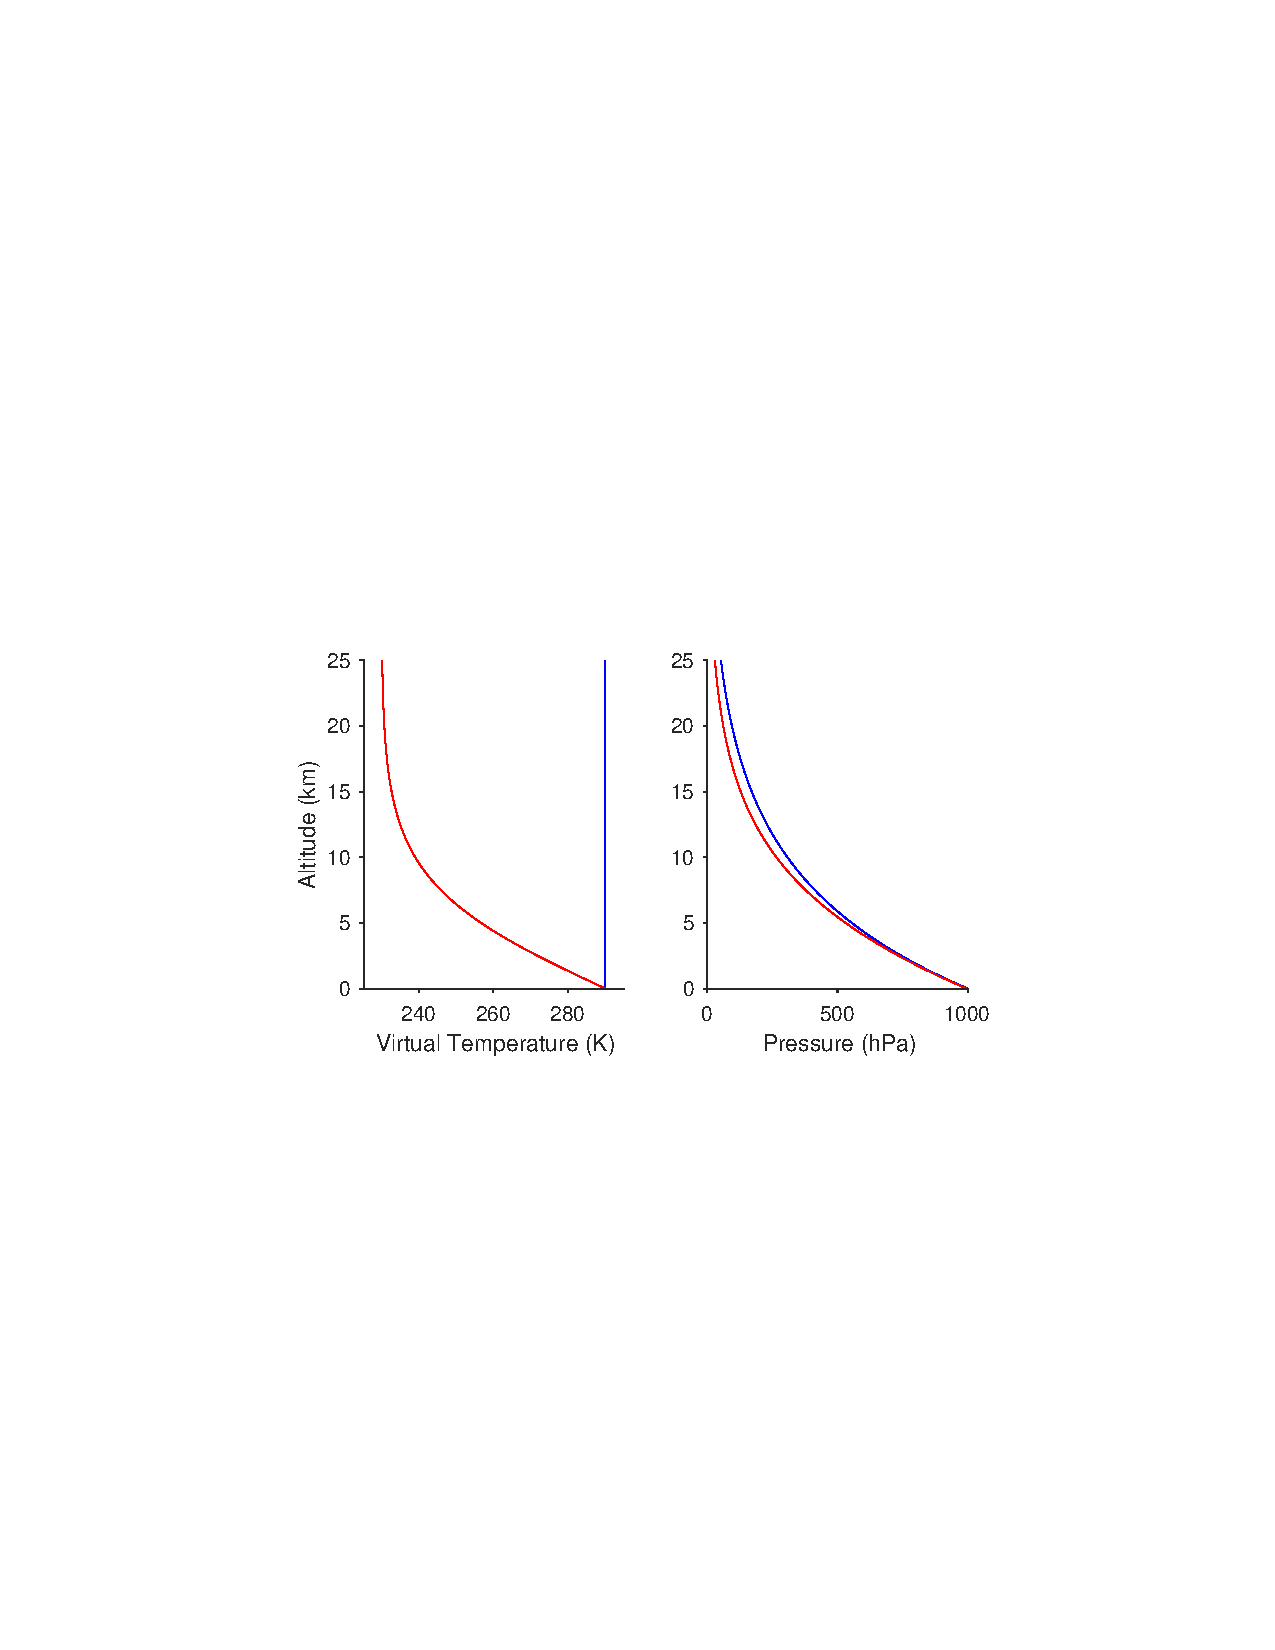
\includegraphics{figures/hydrostatic_state.pdf}
    \caption{(a) An isothermal virtual temperature profile (blue) and a virtual temperature profile \eqref{e:ref_temperature} (red) with surface temperature $T_{v, \mathrm{sfc}} = 290~\mathrm{K}$, temperature drop $\Delta T = 60~\mathrm{K}$, and tropospheric height scale $H_{t} = 8~\mathrm{km}$---values roughly representative of Earth's midlatitude atmosphere. (b) The corresponding hydrostatically balanced pressure profiles \eqref{e:hydro_pressure}, with $p_{\mathrm{MSLP}} = 10^5~\mathrm{Pa} = 1000~\mathrm{hPa}$.}
    \label{f:hydrostatic_state}
\end{figure}

% A simple temperature profile that covers many cases is
% \begin{equation}\label{e:ref_temperature}
%     T_{v,r}(z) = \max \left( T_{v, \mathrm{sfc}} - \Gamma z, T_{\min} \right),
% \end{equation}
% with parameters
% \begin{itemize}
%     \item $T_{v, \mathrm{sfc}}$: surface temperature, 
%     \item $\Gamma$: temperature lapse rate at temperatures below $T_{\min}$,
%     \item $T_{\min}$: minimum temperature.
% \end{itemize}
% This temperature decreases linearly in $z$ at a lapse rate $\Gamma$ from the surface temperature $T_{v, \mathrm{sfc}}$ to the minimum temperature $T_{\min}$, attained at 
% \begin{equation}\label{e:z_t}
% z_{t} = \frac{T_{v, \mathrm{sfc}} - T_{\min}}{\Gamma}.
% \end{equation}
% The temperature is constant and equal to $T_{\min}$ above $z_t$. See Fig.~\ref{f:hydrostatic_state}a for an example. The resulting temperature profile is a rough approximation of a tropospheric temperature profile with lapse rate $\Gamma$ and a ``tropopause'' at height $z_t$, overlain by a ``stratosphere'' with constant temperature $T_{\min}$. For $\Gamma = g/c_{pd}$, the ``tropospheric'' temperature profile is dry adiabatic (isentropic), i.e., has constant (dry) potential temperature. 

\subsection{Pressure}

The pressure $p_r(z)$ consistent with the virtual temperature profile $T_{v,r}(z)$ is obtained by combining hydrostatic balance ($\partial_z p_r(z) = - \rho_r g$) with the ideal gas law ($p_r =\rho_r R_d T_{v, r}$). This gives $\partial_z \log(p_r) = -g/(R_d T_{v, r})$, or
\begin{equation}\label{e:hydro_pressure_gen}
p_r(z) = p_{\mathrm{MSLP}} \exp\left(-\int_0^z \frac{g}{R_d T_{v, r}(z')} dz' \right),
\end{equation}
where we have chosen for the pressure $p_r(0)$ at altitude $z=0$ the mean sea-level pressure $p_{\mathrm{MSLP}}$, a model parameter. 

Integrating \eqref{e:hydro_pressure_gen} with the virtual temperature profile \eqref{e:ref_temperature} leads to
\begin{multline}\label{e:hydro_pressure}
p_r(z) = p_{\mathrm{MSLP}}\\
 \times \exp\left\{
% -\frac{z + H_{t} \Delta T' 
% \log\left[ \cosh\left(\frac{z}{H_{t}}\right) - \atanh(\Delta T')\right]}%
% {H_{\mathrm{sfc}}[1 - (\Delta T')^2]}
 -\frac{z + H_{t} \Delta T' \left[
 \log \left(1-\Delta T' \tanh\left(\frac{z}{H_{t}}\right)\right) -
 \log\left(1 + \tanh\left(\frac{z}{H_{t}}\right)\right) + \frac{z}{H_t}\right]}%
 {H_{\mathrm{sfc}}[1 - (\Delta T')^2]}
\right\}
\end{multline}
where $\Delta T' = \Delta T/T_{v, \mathrm{sfc}}$ is the fractional temperature drop and \begin{equation}
H_\mathrm{sfc}  = \frac{R_d T_{v,\mathrm{sfc}}}{g}
\end{equation}
is the density scale height at the surface. 

\subsection{Density}
 
Given the virtual temperature $T_{v,r}(z)$ and hydrostatic pressure $p_r(z)$, the reference density $\rho_r(z)$ follows from the ideal gas law as
\begin{equation}\label{e:hydro_density}
    \rho_r(z) = \frac{p_r(z)}{R_d T_{v,r}(z)}.
\end{equation}
This holds exactly for continuous $z$.

To obtain reference states that are in discrete hydrostatic balance, one can compute the density by differentiating pressure discretely,
\begin{equation}\label{e:hydro_density_discrete}
    \rho_r(z) = -\frac{1}{g} \frac{\partial p_r(z)}{\partial z}.
\end{equation}
The density so computed, with a discrete derivative of pressure, is guaranteed to be in hydrostatic balance with the pressure $p_r(z)$. A virtual temperature that is discretely consistent with this density can then be computed from the ideal-gas law as $T_{v,r}(z) = p_r(z)/[R_d \rho_r(z)]$. This ensures a hydrostatic reference pressure, density, and temperature in discrete hydrostatic balance. Naturally, for a polynomial approximation of degree $n$ for pressure, the polynomial approximation for density and temperature will be of degree $n-1$ and may be discontinuous at element interfaces in discontinuous Galerkin discretizations. Alternatively, continuous densities and pressures in discrete hydrostatic balance can be ensured by computing the pressure $p_r(z)$ by discrete integration of Eq.~\eqref{e:hydro_pressure_gen}, with a discrete integration that is the exact inverse of the discrete differentiation used in the model.

The pressure \eqref{e:hydro_pressure} and density \eqref{e:hydro_density} or \eqref{e:hydro_density_discrete} together specify a family of smooth reference states that can be used to factor out a hydrostatic reference state in the momentum balance \eqref{e:governing_equations/momentum}. Relative or specific humidities, or the actual temperature, are not needed in the momentum balance.

\subsection{Temperature and Specific Humidities}

For initialization of the model and as a reference state for linearizations for linear implicit time stepping, we need a complete thermodynamic specification of the reference state, including the humidities and temperature needed to specify the internal energy of the reference state. For a dry reference state ($\mathrm{RH}=0$), the temperature is equal to the virtual temperature, $T_r  = T_{v,r}$, and specification of the full thermodynamic state is straightforward. 

More generally, we wish to specify a relative humidity $\mathrm{RH}$ in the reference state such that the total specific humidity $q_{t, r}(z)$, temperature $T_{r}(z)$, and density $\rho_r(z)$ are related by
\begin{equation}\label{e:qt_given_RH}
    q_{t,r}(z) = \mathrm{RH} \, q_v^*\bigl( T_{r}(z), \rho_r(z) \bigr).
\end{equation}
Here, $q_v^*(T_r, \rho_r)$ is the saturation specific humidity \eqref{e:sat_shum}, which depends on the reference temperature $T_r(z)$ and density $\rho_r(z)$. The reference temperature $T_r$, in turn, is related to the reference virtual temperature $T_{v, r}$ through the definition of the virtual temperature \eqref{e:virtual_temp},
\begin{equation}\label{e:temp_from_virt_temp}
R_m(q_r) T_r - R_d T_{v, r} = 0,
\end{equation}
where the moist gas constant $R_m(q_r)$ depends on the reference specific humidities $q_r=(q_{t,r}, q_{l, r}, q_{i, r})$ through its definition \eqref{e:R_m}. That is, for $\mathrm{RH}>0$, computing the temperature $T_r$ from the virtual temperature $T_{v, r}$ is a nonlinear problem that must be solved iteratively by finding roots of \eqref{e:temp_from_virt_temp} subject to the total specific humidity specification \eqref{e:qt_given_RH}, through a saturation adjustment procedure similar to that described in section~\ref{sct:sat_adj}. We allow $\mathrm{RH} > 1$ to be able to have supersaturated states with nonzero condensate specific humidities $q_{l, r}$ and $q_{i, r}$. 

In Earth's atmosphere, the temperature only deviates from the virtual temperature by $O(1~\mathrm{K})$, so as a reference state for linearization in implicit timestepping, choosing a state with $\mathrm{RH}=0$ and $T_r = T_{v, r}$ suffices. For initialization of a model with nonzero specific humidity in the initial state, the nonlinear problem \eqref{e:temp_from_virt_temp} needs to be solved to completely specify a balanced initial state.

\section{Dry Adiabatic Reference State}

For simulations in limited domains, a dry adiabatic reference state is often used for initialization. This corresponds to a reference temperature that decreases linearly with height at the dry adiabatic lapse rate $g/c_{pd}$,
\begin{equation}\label{e:temperature_adiabat}
    T_r = T_{r, \mathrm{sfc}} - \frac{g}{c_{pd}} z.
\end{equation}
The corresponding pressure is
\begin{equation}\label{e:pressure_adiabat}
p_r(z) = p_{\mathrm{MSLP}} 
\left(1 - \frac{g z}{c_{pd} T_{v, \mathrm{sfc}}} \right)^{c_{pd}/R_d}.
\end{equation}
The density again follows from the ideal gas law,
\begin{equation}
    \rho_r(z) = \frac{p_r(z)}{R_d T_r(z)},
\end{equation}
thus completing the specification of the dry-adiabatic reference state.

\section{Energy}

From the above definitions of the reference temperature $T_r$ and, where applicable, the specific humidities $q_r$ we can compute the specific internal energy $I_r$ in the reference state using Eq.~\eqref{e:total_internal_energy}, and with that the total specific energy $e^{\mathrm{tot}}_r = I_r + \Phi$ corresponding to a state of rest ($\vec{u}=0$). This completes the specification of the thermodynamics of the reference state.

\section{Noise}

It is common to add a small amount of random noise, e.g., to the initial (virtual) temperature or energy at the surface, to break the symmetry of the initial state and allow three-dimensional instabilities to develop. A typical standard deviation of such noise may be 1\% of the reference values at the surface.

\chapter{Benchmark Cases}\label{c:benchmarks}

Here we describe a suite of test cases for dry and moist atmospheres, and for coarse-resolution global and higher-resolution limited-area model configurations. 

\section{Held-Suarez (1994) Dry GCM Benchmark}

\citet{Held94} describe a simple and widely used setup for testing dry dynamical cores of GCMs. This setup is usually used to focus on statistically steady states (reached after about 100--400~days of spinup) but also lends itself to the study of the time-dependent evolution of Rossby waves and baroclinic instability. In this benchmark calculation, vertical SGS fluxes are usually set to zero; however, horizontal hyperdiffusion is needed to damp the enstrophy cascade. 

\subsection{Initial Condition}

The initial condition for the Held-Suarez benchmark is an isothermal atmosphere at rest, with $T(t=0) = 300~\mathrm{K}$. Hydrostatically balanced initial density and pressure fields are calculated from the initial temperature according to section~\ref{c:reference_state}, and some small random perturbations are added to the density field to break the symmetry of the initial state and allow 3D baroclinic waves to develop. Baroclinic waves develop within a few simulated days in this benchmark calculation, and they begin to equilibrate after around 20--30~days. 

\subsection{Boundary Conditions}

The lower boundary condition is free-slip and thermally insulating, with no evaporation. That is, \emph{all} diffusive fluxes at the lower boundary (see section~\ref{s:bottom_bc}) are taken to be zero (if they are not already taken to be zero throughout the atmosphere, which is common in the Held-Suarez benchmark). With the vanishing surface fluxes, there is no need to specify a surface temperature.

\subsection{Sources}

\subsubsection{Momentum} 

Bottom drag in this benchmark calculation is modeled as a momentum sink in the lower part of the atmosphere, which is a function of velocity $\vec{u}$ and pressure $p$. The momentum sink takes the form of linear Rayleigh drag
\begin{equation}
    \vec{F}_{\vec{u}} = -k_v(\sigma) \vec{u}_p,
\end{equation}
where $\vec{u}_p = (\vec{I} - \vec{\hat n}\vec{\hat n}^T)\vec{u}$ is the velocity component parallel to the surface (the horizontal velocity at a plane surface) and the drag coefficient decays away from the surface:
\begin{equation}
    k_v(\sigma) = k_f \max \left( 0, \frac{\sigma - \sigma_b}{1-\sigma_b} \right).
\end{equation}
Here,
\[
\sigma = \frac{p}{p_{\mathrm{sfc}}}
\]
is pressure normalized by the temporally and spatially varying surface pressure $p_{\mathrm{sfc}}$. \hl{[This still needs to be fixed in the code.]} The two parameters are
\begin{itemize}
    \item $\sigma_b = 0.7$: vertical extent of drag layer
    \item $k_f = 1~\mathrm{day^{-1}}$: drag coefficient at the surface
\end{itemize}.

\subsubsection{Heating/cooling}

Radiative heating/cooling is represented by linear relaxation of temperatures toward a radiative-equilibrium state with temperature \hl{[Note that here $p/p_{\mathrm{MSLP}}$ should be this, with a constant pressure for normalization. So generally, this is not equal to $\sigma$ above; it is only equal with the simplified $\sigma$ above.]}
\begin{multline}
    T_{\mathrm{eq}} = \max \\
    \left\{ T_{\mathrm{top}}, \left[ T_{\max} - (\Delta T)_y \sin^2 \phi - (\Delta \theta)_z \log\left(\frac{p}{p_{\mathrm{MSLP}}}\right) \cos^2 \phi \right]
    \left( \frac{p}{p_{\mathrm{MSLP}}} \right)^{\kappa} \right\}.
\end{multline}
Here, $\phi$ is latitude, $\kappa = R_d/c_{pd}$ is the adiabatic exponent, and the default values of the parameters are:
\begin{itemize}
    \item $T_{\mathrm{top}} = 200~\mathrm{K}$: temperature at model top
    \item $T_{\max} = 315~\mathrm{K}$: near-surface temperature at equator
    \item $(\Delta T)_y = 60~\mathrm{K}$: pole-equator temperature difference in radiative equilibrium
    \item $(\Delta \theta)_z = 10~\mathrm{K}$: static stability in background state.
\end{itemize}

Relaxation of temperatures toward the background state on a timescale $k_T^{-1}$ implies a source in the energy equation that is a function of latitude $\phi$, pressure $p$, and temperature $T$:
\begin{equation}
    Q =  - c_{vd} k_T(\phi, p) (T - T_{\mathrm{eq}}).
\end{equation} 
The relaxation coefficient $k_T$ is taken to vary with latitude and normalized pressure $\sigma$ as
\begin{equation}
k_T(\phi, p) = k_a + (k_s - k_a) \max\left(0, \frac{\sigma - \sigma_b}{1-\sigma_b}\right) \cos^4 \phi ,
\end{equation}
where 
\begin{itemize}
    \item $k_a = (40~\mathrm{day})^{-1}$: relaxation coefficient in interior atmosphere
    \item $k_s = (4~\mathrm{day})^{-1}$: relaxation coefficient  at equator near the surface.
\end{itemize}
The interior relaxation timescale $k_a^{-1}$ controls the timescale over which the flow equilibrates to a statistically steady state.

\subsection{SGS Fluxes}
In global models with a stratified atmosphere, large-scale turbulence with Rossby waves usually dominates the kinetic energy of the flow. The large-scale flow is primarily rotational and horizontal. SGS dissipation primarily needs to absorb the cascade of enstrophy (vorticity variance) to small scales. This is usually accomplished by horizontal hyperdiffusion, such as biharmonic diffusion.

Hence, the SGS mixing needs to be strongly anisotropic, e.g., as outlined in chapter~\ref{c:sgs_models}.

\section{2D Rising Thermal Bubble (Robert 1993)}
\label{2dRTBtest}
\cite{robert1993} describes a test of a thermal bubble rising in an isentropic environment. The atmosphere is initially neutrally stratified with uniform potential temperature $\theta_0 = 303~\mathrm{K}$. The initial state is in hydrostatic equilibrium, so that the pressure decreases with $z$ as
\begin{equation}
\label{pressureDistrib}
p = p_{0}\left(1-\frac{g}{c_p{\theta_{0}}}z\right)^{c_p/R}.
\end{equation}
The domain is $[-500~\mathrm{m},500~\mathrm{m}]\times[0,1500~\mathrm{m}]$. 

We consider two different ways of triggering a rising thermal, either through a buoyant bubble specified in the initial condition, or through boundary fluxes that drive a thermal.

\subsection{Buoyant Bubble in Initial Condition}

This is the case originally considered by \cite{robert1993}. The flow is triggered by a Gaussian-shaped potential temperature perturbation with a flat region at the center, defined as
\begin{equation}
 \Delta\theta = \left\{ \begin{array}{ll}
 \theta_c & \text{if } r \leq a\\
 \theta_c e^{-(r - a)^2/\sigma^2} & \text{if } r > a\\
\end{array} \right.
\label{e:robertIni}
\end{equation}
where $r = \sqrt[]{(x-x_{c})^{2} + (z-z_{c})^{2}}$, $(x_c,z_c) = (500,260)\,\mathrm{m}$, $a=50~\mathrm{m}$, $\sigma = 100~\mathrm{m}$, and $\theta_c=0.5~\mathrm{K}$. Results of a simulation of this flow are shown in Fig.~\ref{fig:benchmarks/robert_bubble}.
\begin{figure}
\centerline{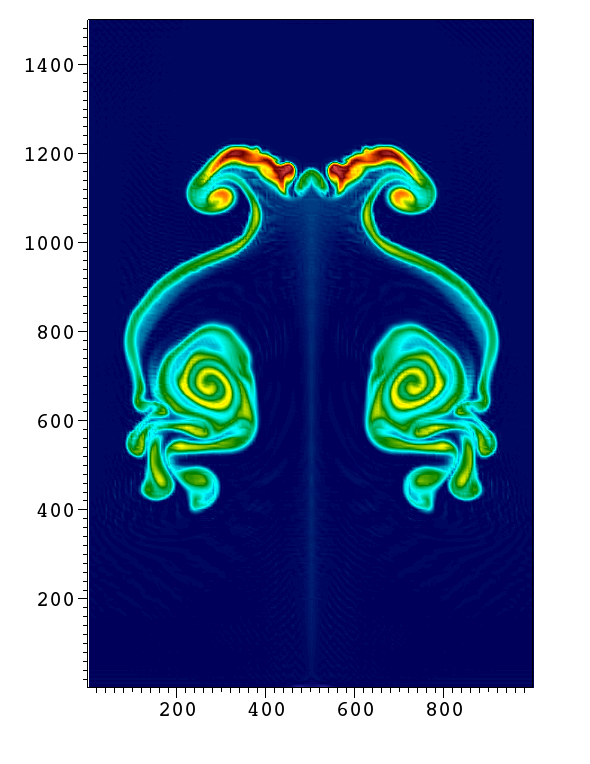
\includegraphics[width=0.7\textwidth]{figures/benchmarks/rtb/RTB-Robert--smgo-5mX5m-1080s0000.png}}
\caption{Simulation of 2D rising thermal bubble triggered by initial perturbation. What is shown is the potential temperature $\theta$ at $t=1080\,\mathrm{s}$. The grid resolution is $\Delta x = \Delta z = 5\,\mathrm{m}$ using $4^{th}$-order polynomials. The simulation is stabilized with a constant coefficient Smagorinsky-Lilly SGS model.}
\label{fig:benchmarks/robert_bubble}
\end{figure}

\subsection{Thermal Driven by Boundary Fluxes}

\subsubsection{One Plume}
An alternative way of driving a thermal is by specifying a heat flux at the lower boundary. This amounts to specifying the moist static energy flux at the surface,
\begin{equation}
    \vec{\hat n} \cdot \rho (\vec{J} + \vec{D})_\mathrm{sfc} = \mathrm{MSEF}(\vec{x}, t).
\end{equation}
To mimic the structure of the thermal bubble specified through the initial condition, one option is to use the moist static energy flux
\begin{equation}
     \mathrm{MSEF}(\vec{x}, t) =  F_0(t) \times \left\{ \begin{array}{ll}
 1 & \text{if } r \leq a\\
 e^{-(r - a)^2/\sigma^2} & \text{if } r > a,\\
\end{array} \right.
\end{equation}
where $r = |x-x_{c}|$, $x_c = 500\,\mathrm{m}$, $a=50~\mathrm{m}$, and $\sigma = 100~\mathrm{m}$. The amplitude of the surface energy flux $F_0(t)$ varies with time as
\begin{equation}
   F_0(t) =
   200~\mathrm{W~m^{-2}}\times 
   \left\{ \begin{array}{ll}
 0 & \text{if } t \leq t_0\\
 1 & \text{if } t_0 < t < t_1,\\
 0 & \text{if } t > t_1,
 \end{array}\right.
\end{equation}
where $t_0=0$ and $t_1 = 500~\mathrm{s}$ (that is, the energy flux at the surface has a top-hat profile in time). 

\subsubsection{Multiple Plumes}

To assist in weak-scaling tests, a heat flux at the lower boundary that is periodic in space can also be prescribed, to allow the generation of multiple plumes in larger domains. In that case, the moist static energy flux is given by
\begin{equation}
\mathrm{MSEF}(\mathbf{x},t) = 
   100~\mathrm{W~m^{-2}}\times \cos^2{\Big(\frac{2\pi x}{x_{0}}\Big)}\times \cos^2{\Big(\frac{2\pi y}{y_{0}}\Big)} \times
   \left\{ \begin{array}{ll}
    1 & \text{if } t_0 \leq t < t_1,\\
    0 & \text{if } t > t_1, \\
     \end{array}\right.
\end{equation}
The parameters $x_{0}$ and $y_{0}$ are parameters control the number of plumes in the domain.  

The surface stress is taken to be zero (free-slip boundary condition). In the standard dry case, evaporation is also taken to be zero. Generalizations with nonzero evaporation, to trigger a moist thermal and possibly a cloud as in section~\ref{s:rtb_moist}, are also possible. 

\section{2D Density Current}

\hl{What follows is still incomplete.}
This test is described in \cite{strakaWilhelmson1993}. It consists of a flow that is triggered by the cold perturbation of a neutrally stratified atmosphere at initially uniform potential temperature $\theta_0 = 300$ K
and in hydrostatic equilibrium such that the pressure decreases with $z$ as:
\begin{equation}
\label{pressureDistrib2}
p = p_{0}\left(1-\frac{g}{c_p{\theta_{0}}}z\right)^{c_p/R}.
\end{equation}
The domain $[-25600,25600]\times[0,6400]\,\mathrm{m}^2$.
The perturbation is linear and defined as
\begin{equation}
 \Delta\theta = \left\{ \begin{array}{ll}
 0 & \mathrm{if } r > 1\,{\mathrm K}\\
 0.5 \theta_c \left(1 + \cos(\pi r) \right) \leq 1\,{\mathrm K}\\
\end{array} \right.
\label{e:robertIni2}
\end{equation}
where $r = \sqrt[]{(x-x_{c})^2/r_x^{2} + (z-z_{c})^{2}/r_z^2}$, $(x_c,z_c) = (0,4000)\,\mathrm{m}$, $(r_x, r_z) = (4000, 2000)\,\mathrm{m}$ and $\theta_c=-15$ K. The fully developed density current at $t=900\,\mathrm{s}$ simulated with a grid effective resolution of $25$ m in both spatial directions is shown in Figure \ref{fig:benchmarks/dc25msmago}.

\begin{figure}
    \centering
    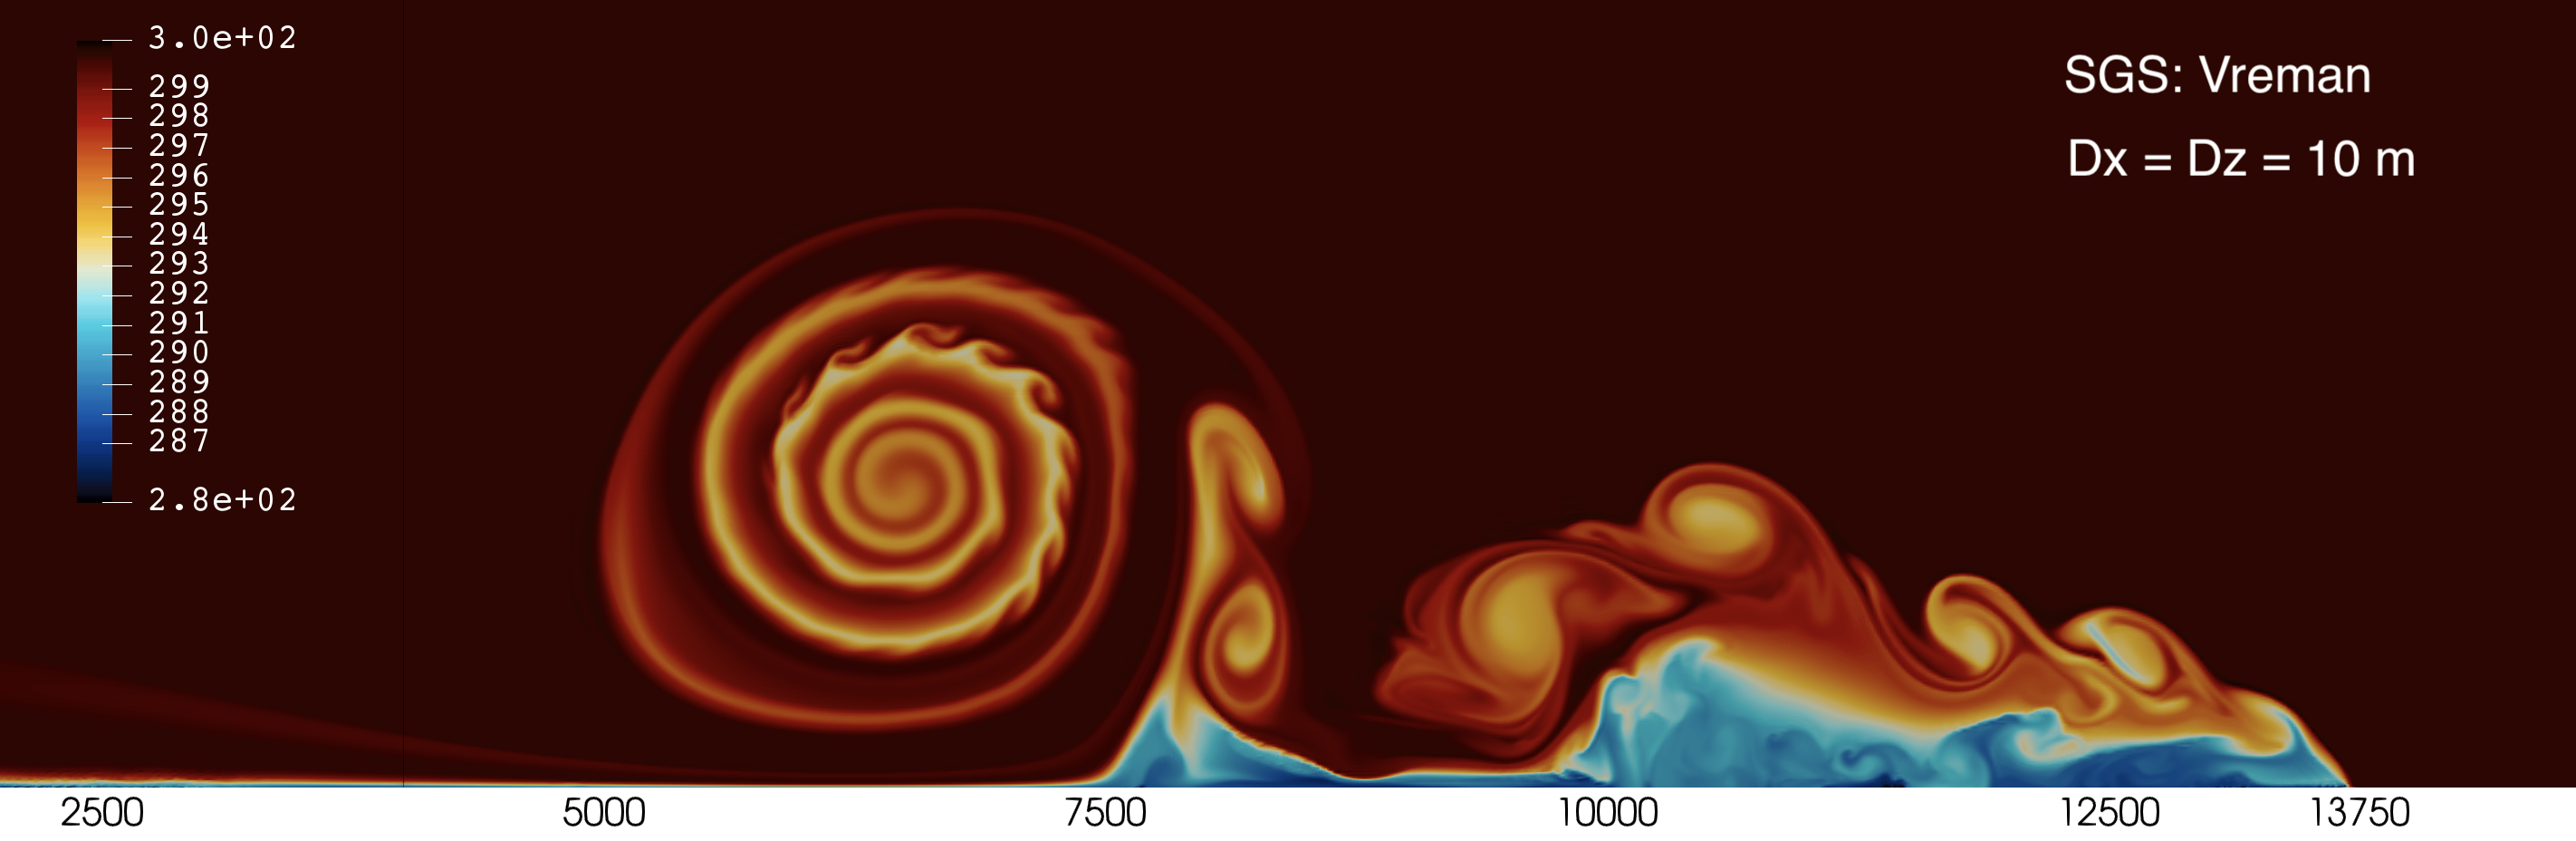
\includegraphics[width=1\textwidth]{./figures/benchmarks/dc/DC_vreman_10m_paraview-notes.png}
    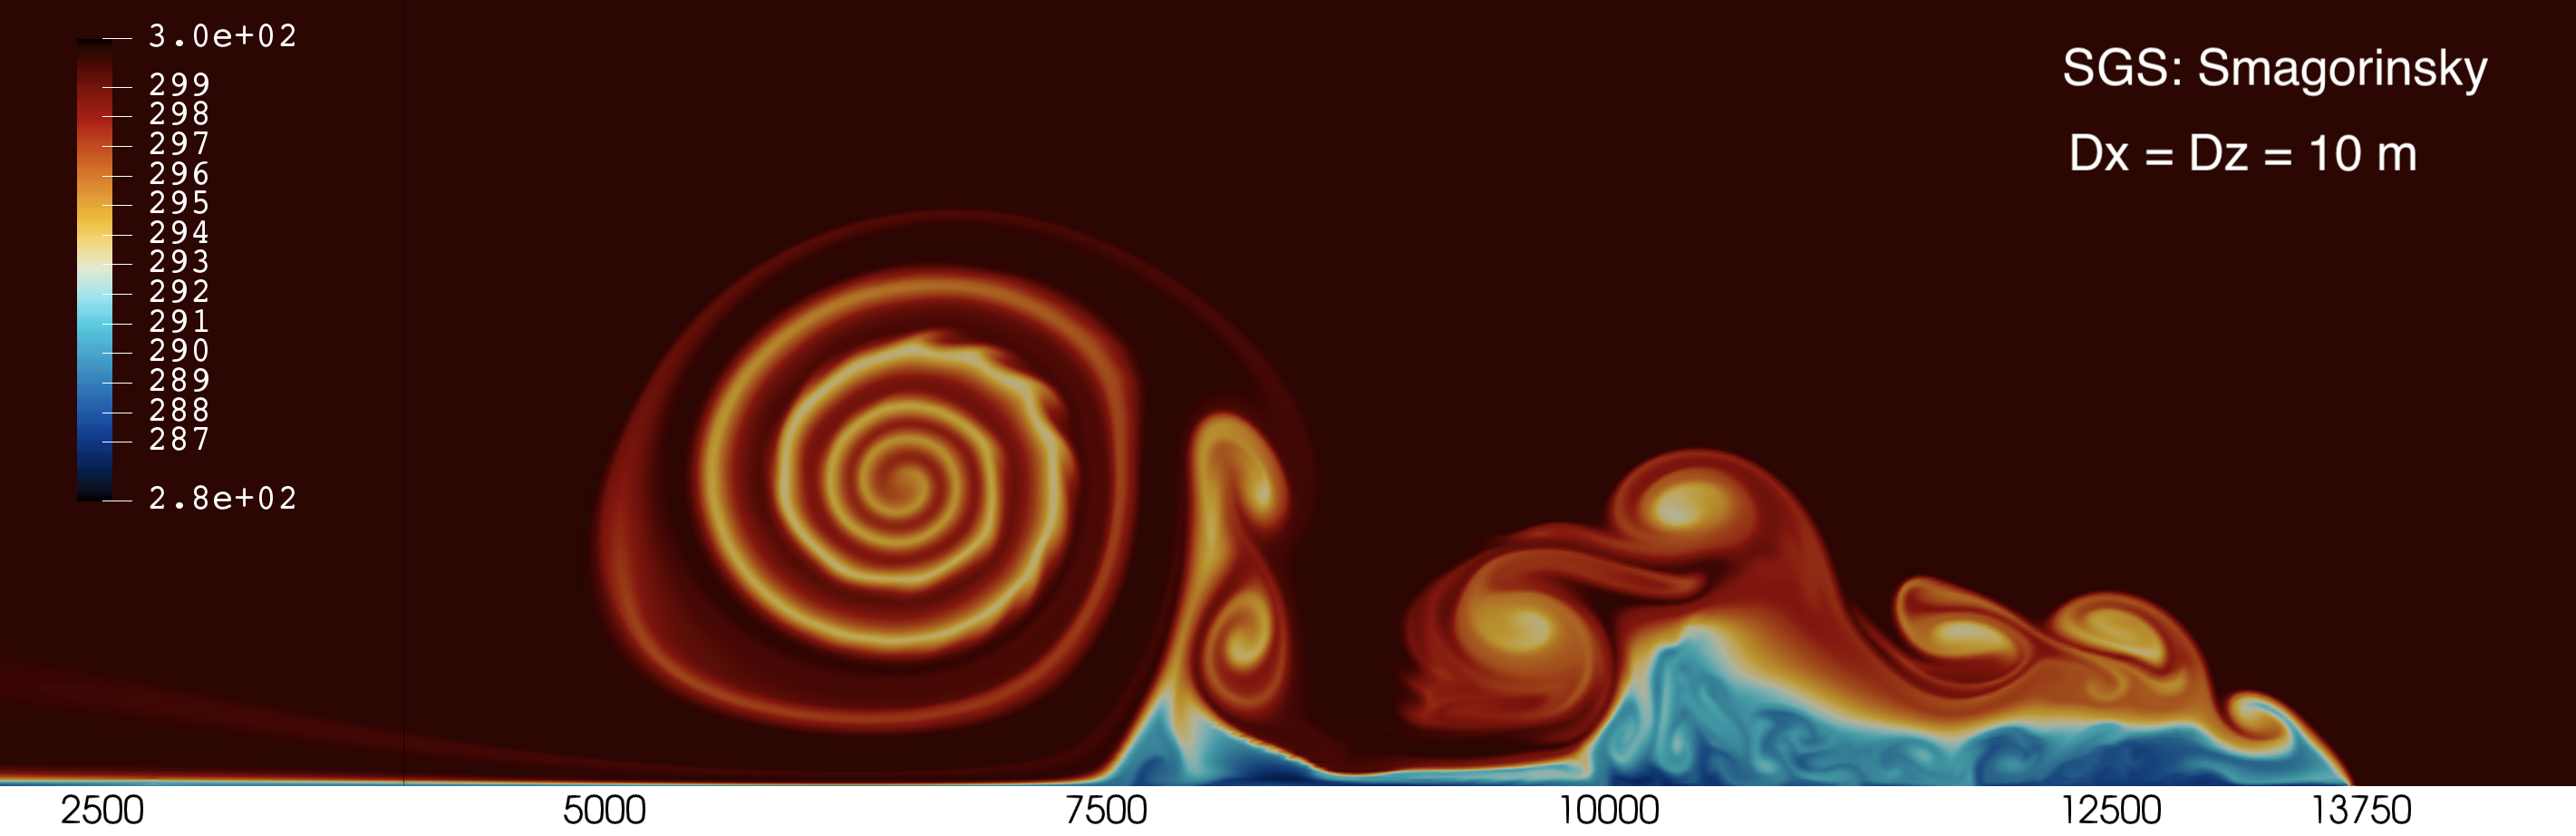
\includegraphics[width=1\textwidth]{./figures/benchmarks/dc/DC_smago_10m_paraview-notes.png}
     \caption{2D$\frac{1}{2}$ density current at 900 seconds computed with effective DG resolutions $\Delta x = \Delta z = 10\,{\rm m}$. Top: Vreman SGS. Bottom: Smagorinsky SGS.}
\label{fig:dc}
\end{figure}

\section{Mountain-triggered gravity waves}
To verify the correct behavior of the DG operator in the presence of non-flat domain and to assess the efficacy of the Rayleigh layer to damp fast moving gravity waves before they reach the top of the domain, a set of steady state mountain-triggered gravity wave problems suggested by \cite{smith1980} are solved. These problems consist of flow with uniform horizontal velocity ${\bf u}= [u,\,0,\, 0]\,{\rm m/s}$ moves eastwards in a doubly periodic domain. A witch-of-Agnesi ideal mountain of height $h_m$ and base length $a$ is centered at $x_c$ and is warped on the bottom boundary according to the function

\begin{equation}
    \label{eq:agnesi}
    z_{sfc} = \frac{h_m a^2}{(x - x_c)^2 + a^2}.
\end{equation}

The background state is in hydrostatic balance with Brunt-V\"ais\"al\"a frequency $\mathcal{N}$ such that

\[
\theta = \theta_{sfc} {\rm e}^{\frac{z\mathcal{N}^2}{g}}
\]
for a given surface potential temperature $\theta_0 = T_0$. The hydrostatically balanced pressure 
\begin{equation}
    \label{eq:pressure_hs_brunt}
    p = p_{sfc}\left[ 1 + \frac{g^2}{c_p\theta_0\mathcal{N}^2}
    \left( {\rm e}^{\frac{-z\mathcal{N}^2}{g}} - 1 \right)  \right]^{c_p/R_{gas}}
\end{equation}
which yields, by means of the gas law, the following density background:

\begin{equation}
    \label{eq:pressure_hs_brunt}
    \rho = \frac{p_{sfc}}{\theta R_{gas}}\left(\frac{p}{p_{sfc}}\right)^{c_v/c_p}.
\end{equation}

\subsection{Linear hydrostatic}
The linear hydrostatic case consists of a neutrally stratified isothermal atmosphere with $\theta=\theta_{sfc} = T=250\,{\rm K}$. Because it is isothermal, the Brunt-V\"ais\"al\"a frquency is 
\[
\mathcal{N} = \frac{g}{\sqrt{c_p T_0}}.
\]
The flow moves in a periodic channel along the $x$-direction with velocity ${\bf u}={20, 0, 0}\,{\rm m/s}$ over a mountain with $h_m=1\,{\rm m}$ and $10,000\,{\rm m}$. A Rayleigh absorbing layer is added at $z_s=25\,{km}$; the layer absorption coefficient is defined as 
\[
\tau_s = \alpha * \sin\left(0.5\pi \frac{z - z_s}{H - z_s} \right)^2,
\]
where we took $\alpha=0.5\,{s}$ and domain top $H=30\,{\rm km}$.

The domain extends from $0$ to $240\,{\rm km}$ in the horizontal direction. 

The steady state solution at $t=15,000$ seconds is shown in the left panel of Figure~\ref{fig:mountainWaves}.

\subsection{Linear non-hydrostatic}
The linear non-hydrostatic mountain waves are forced by a flow of uniform horizontal velocity $u=10\,{\rm m/s}$ over a mountain with $h_m=1\,{\rm}$ and $a=1,000\,{\rm m}$.


The steady state solution at $t=18,000$ seconds is shown in the right panel of Figure~\ref{fig:mountainWaves}.

\begin{figure}
    \centering
    %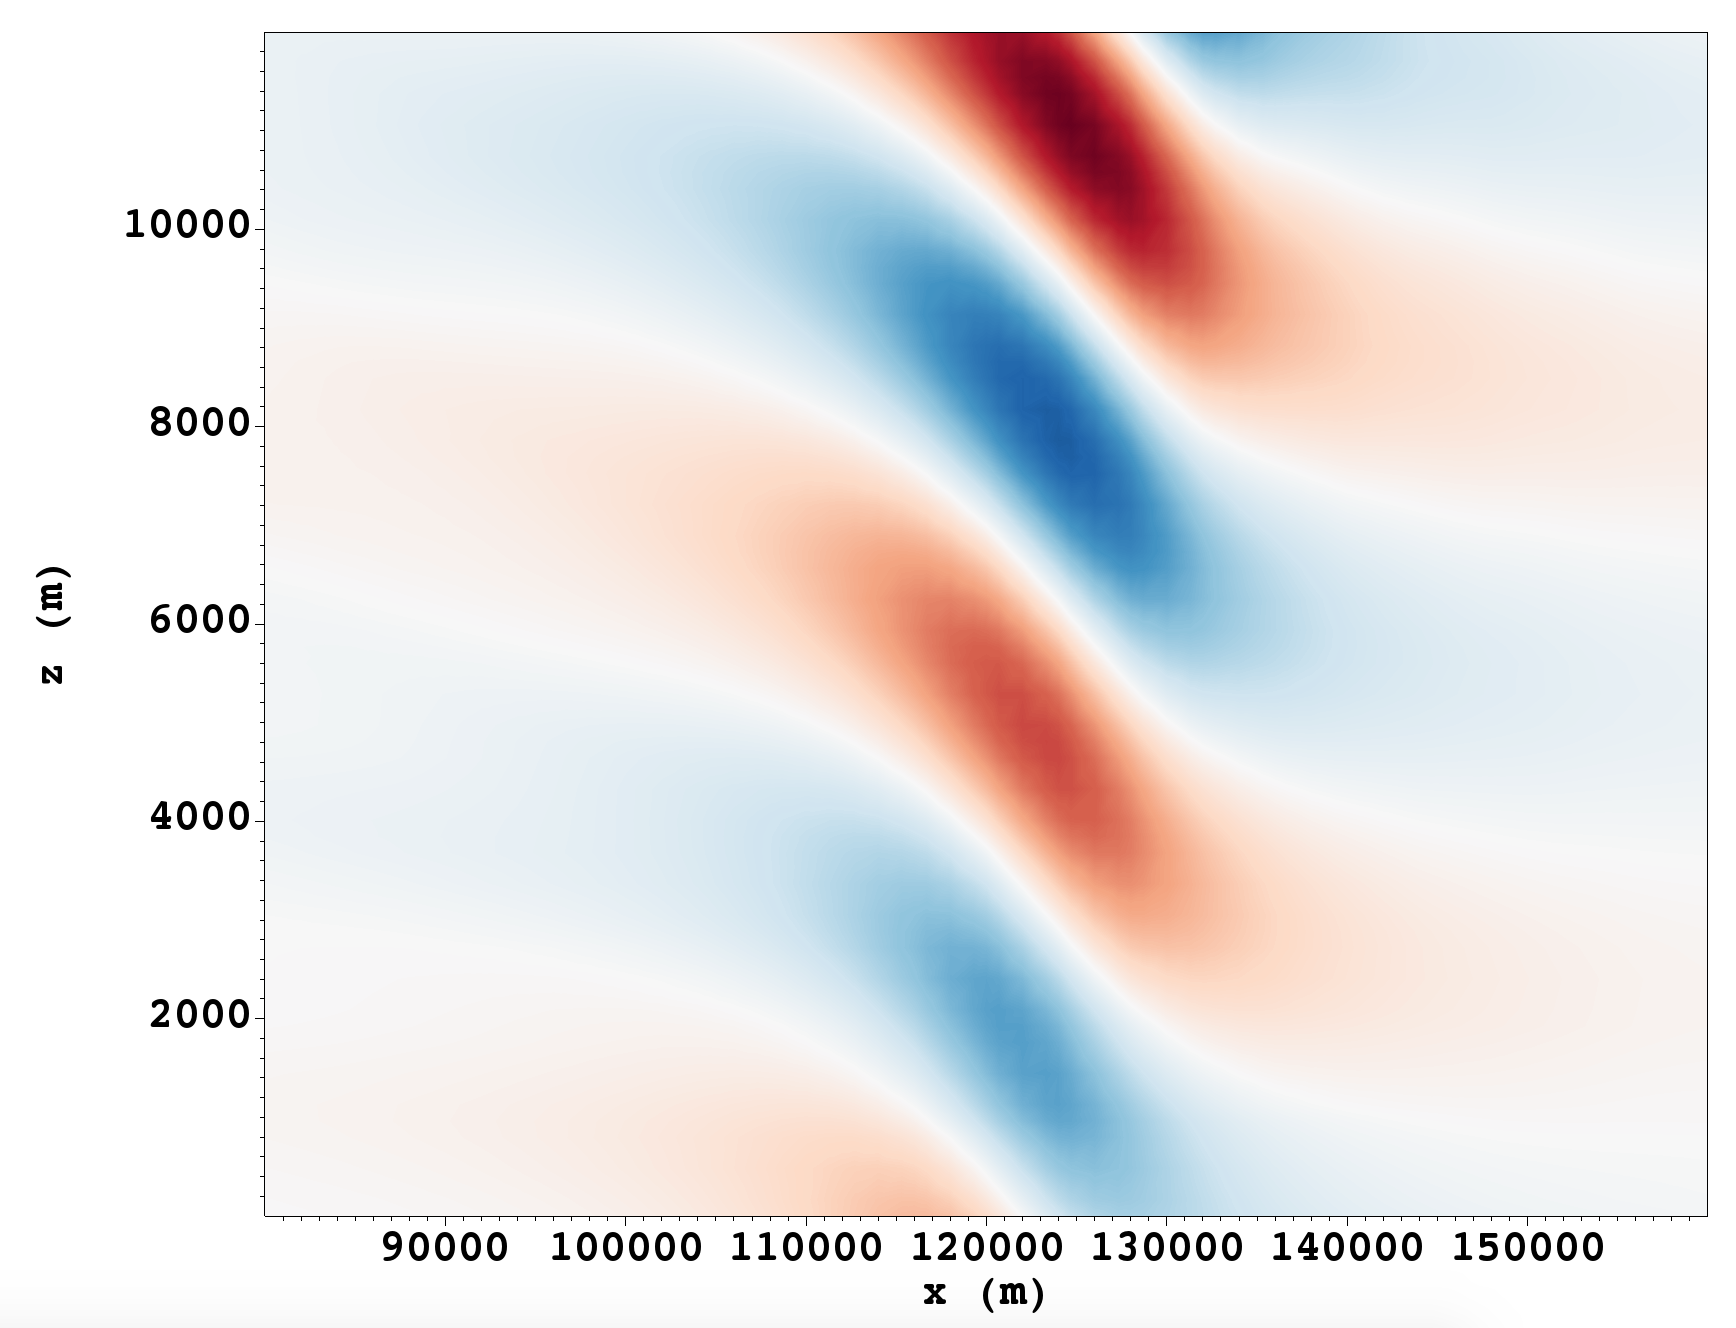
\includegraphics[width=0.49\textwidth]{./figures/benchmarks/mountain_waves/LHS-color.png}
    %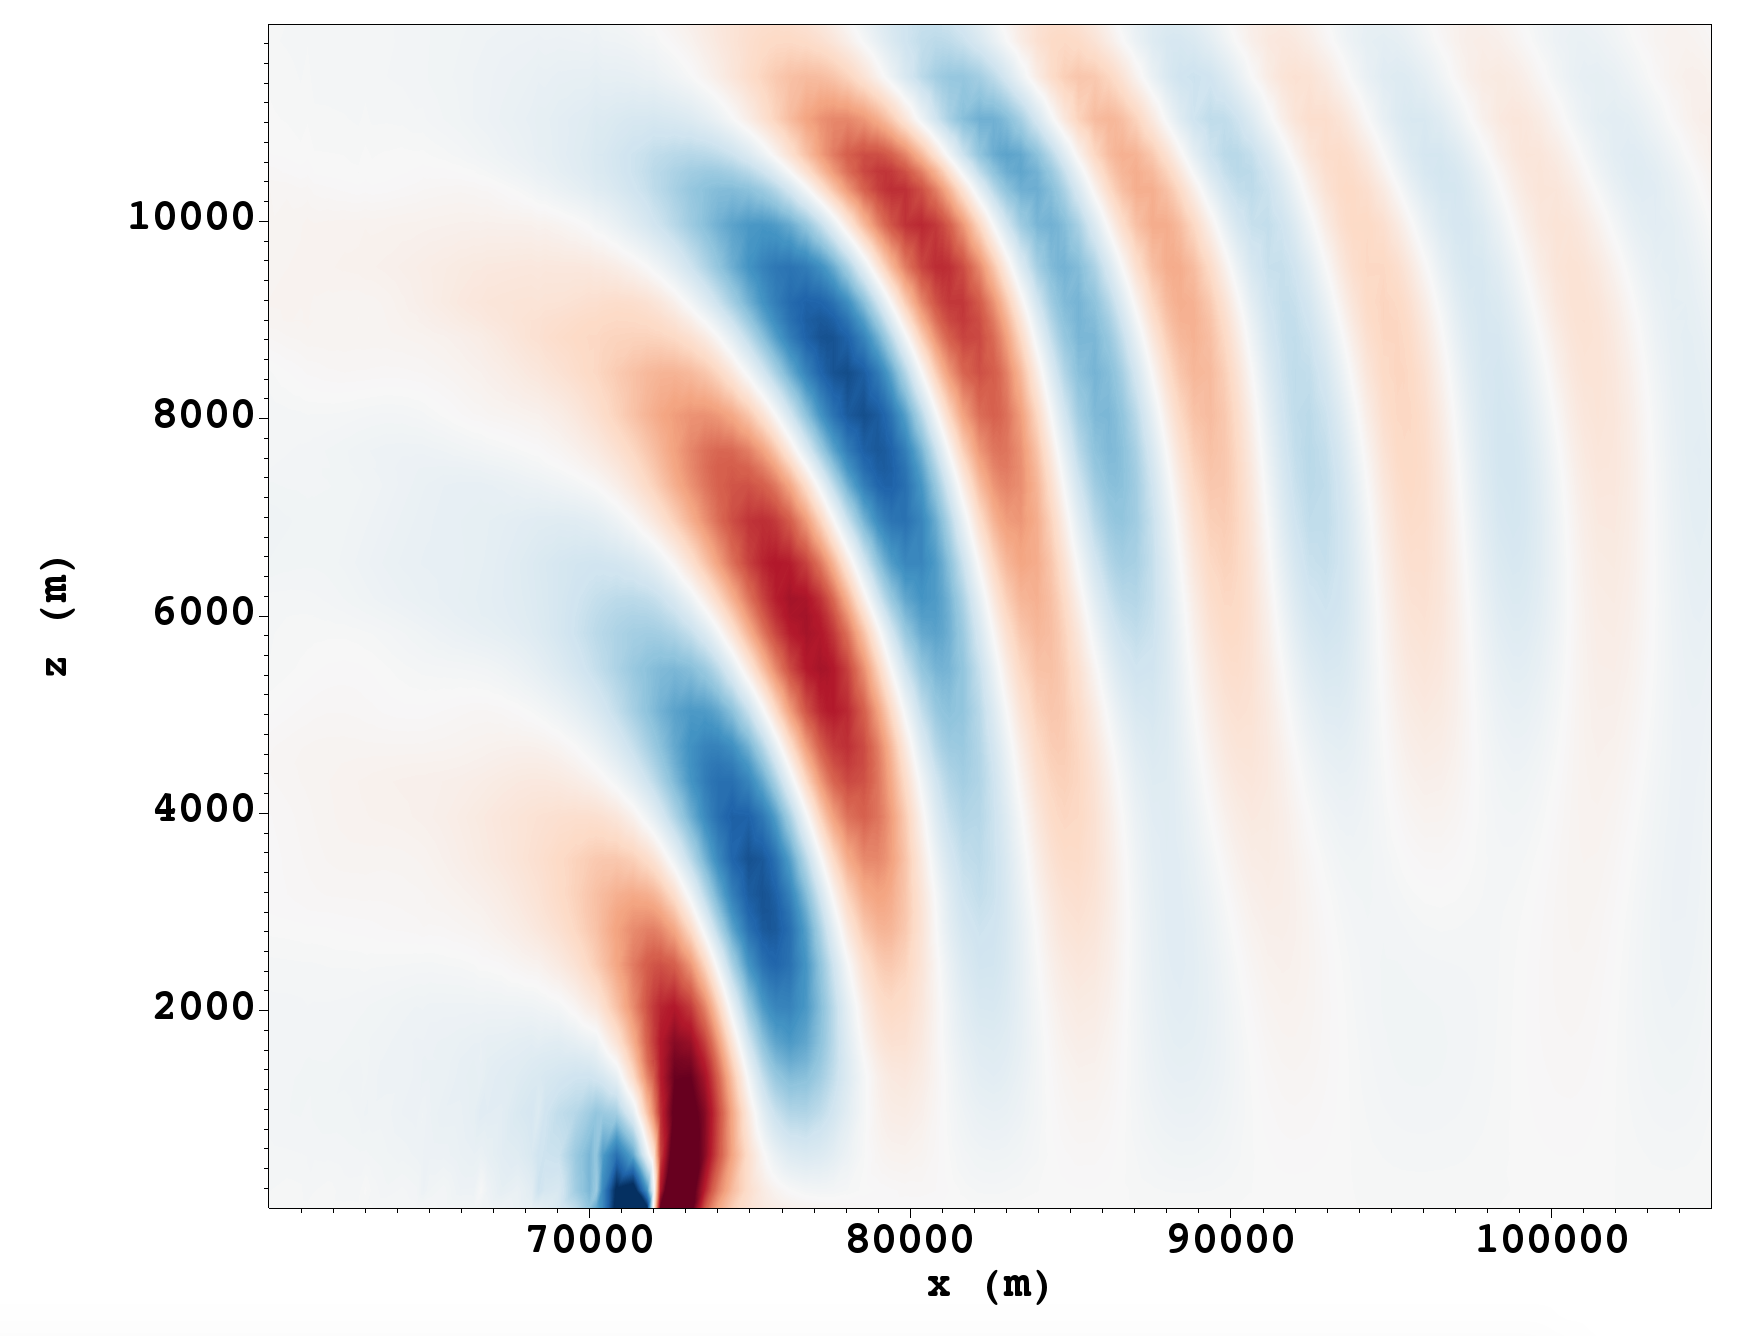
\includegraphics[width=0.49\textwidth]{./figures/benchmarks/mountain_waves/LNH-color.png}
    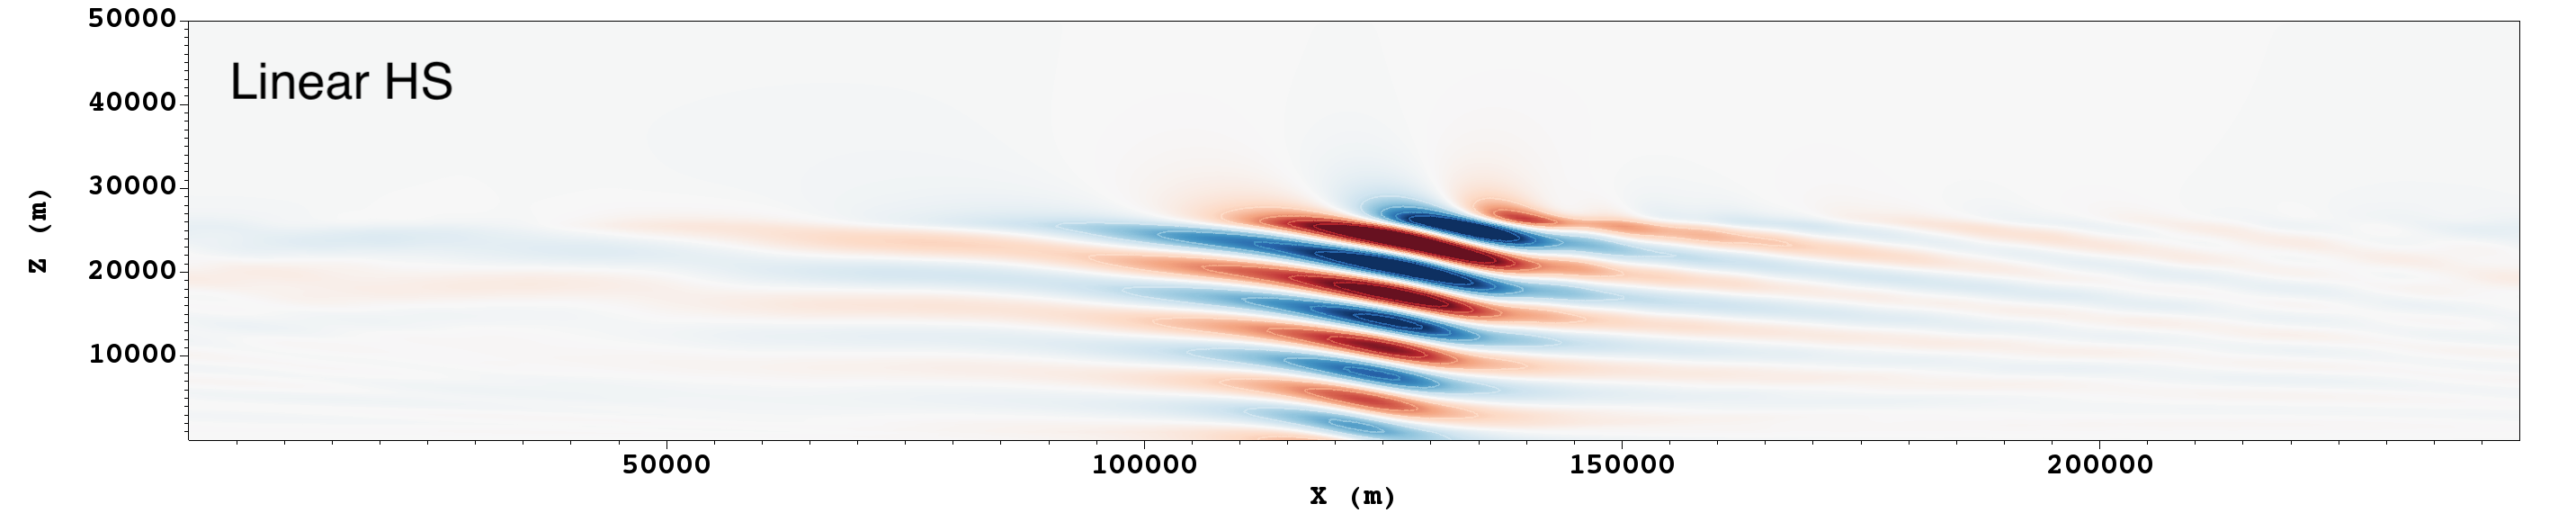
\includegraphics[width=\textwidth]{./figures/benchmarks/mountain_waves/LHS-color-full-domain-500mx240m-notes.png}
    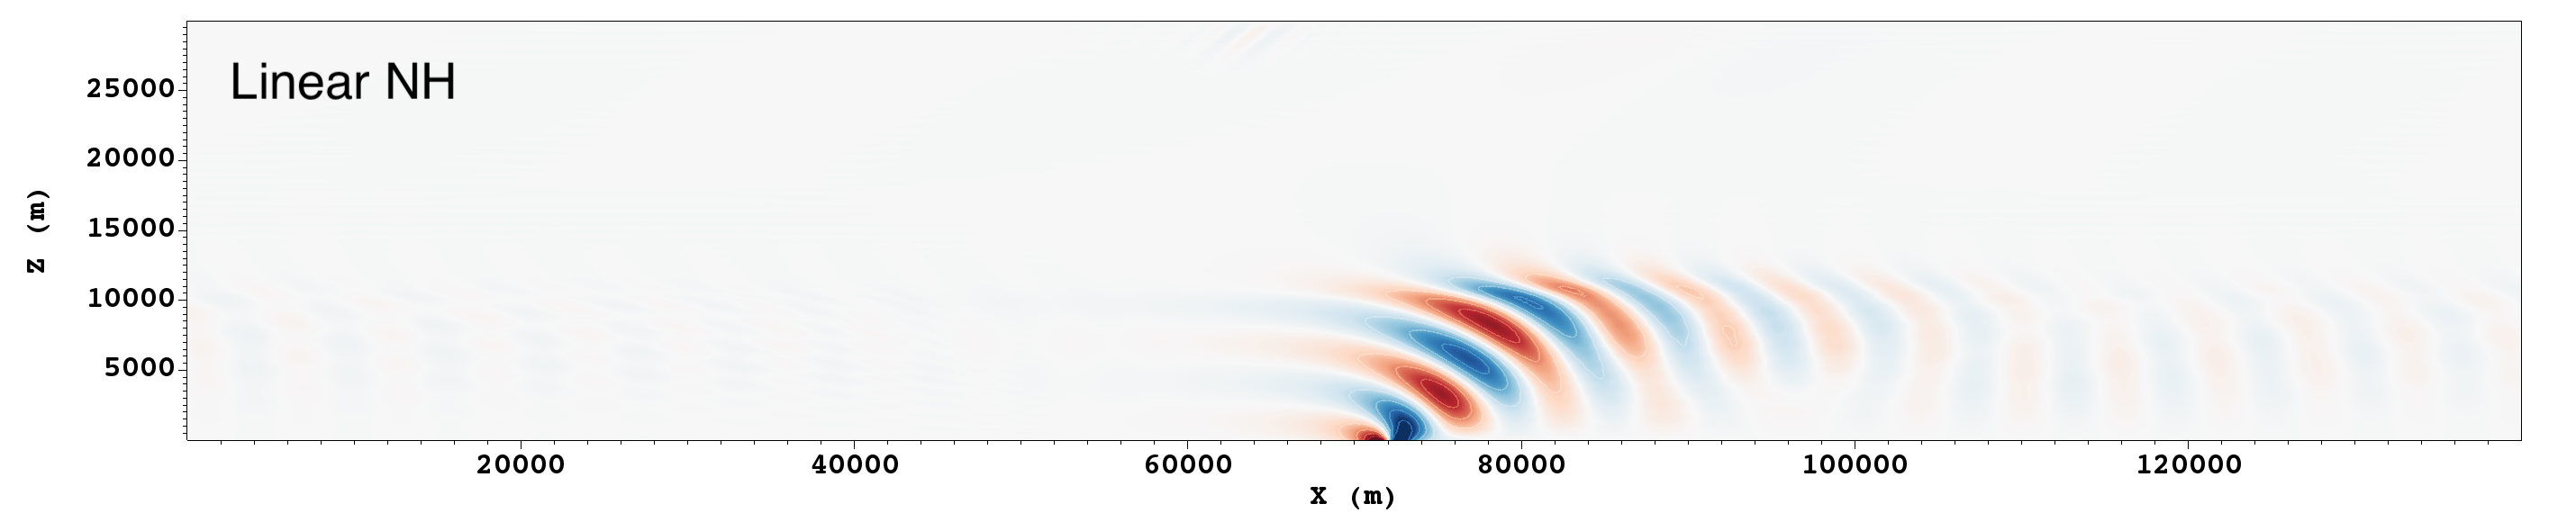
\includegraphics[width=\textwidth]{./figures/benchmarks/mountain_waves/LNH-color-full-domain-200mx160m-notes.png}
     \caption{Vertical velocity $w$ for two linear mountain wave tests. Left:  hydrostatic test at $t=15,000$ seconds. 
     Left: The contours are shown in the range $-4e-3 < w ({\rm m/s})< +4e-3$. The results are shown for effective horizontal resolution $\Delta x=500\,{m}$ and effective vertical resolution $\Delta x=240\,{m}$ using $4^{th}$-order elements.
     Right: non-hydrostatic test at $t=18,000$ seconds. The contours are shown in the range $-4.8e-3 < w ({\rm m/s}) < +4.8e-3$. The results are shown for effective horizontal resolution $\Delta x=200\,{m}$ and effective vertical resolution $\Delta x=160\,{m}$ using $4^{th}$-order elements. The full domain is shown to identify the effectiveness of the Rayleigh absorbing layer.}
\label{fig:mountainWaves}
\end{figure}



%%

%%
\section{Barbados Oceanographic and Meteorological Experiment: BOMEX}

This is a case of shallow, non-precipitating cumulus convection, modeled on a field study off Barbados in 1969. The LES setup consists of a 6.4km $\times$ 6.4km (horizontal) $\times$ 3km (vertical) domain, with effective resolutions of 100m in the horizontal, and 40m in the vertical coordinate. 

\subsection{Initial Condition}

\cite{Siebesma2003} provides the following initial distributions:
\begin{itemize}
    \item Liquid water potential temperature (K)
\begin{equation}\label{e:bomex_init_thetal}
\theta_l(z) = 
    \begin{cases}
    298.7 & z\leq z_{i1},\\
    298.7 + (302.4-298.7)\frac{z - z_{i1}}{z_{i2} - z_{i1}} &  z_{i1} < z \leq z_{i2}, \\
    302.4 + (308.2-302.4)\frac{z - z_{i2}}{z_{i3} - z_{i2}} &  z_{i2} < z \leq z_{i3}, \\
    308.2 + (311.85-308.2)\frac{z - z_{i3}}{z_{i4} - z_{i3}} &  z > z_{i3}.
    \end{cases}
\end{equation}
\item Total specific humidity ($\mathrm{g~kg^{-1}}=10^{-3}$)
\begin{equation}\label{e:bomex_init_qt}
q_t(z) = 
    \begin{cases}
    17.0 + (16.3-17.0)\frac{z}{z_1} & z\leq z_{i1},\\
    16.3 + (10.7-16.3)\frac{z - z_{i1}}{z_{i2} - z_{i1}} &  z_{i1} < z \leq z_{i2}, \\
    10.7 + (4.2-10.7)\frac{z - z_{i2}}{z_{i3} - z_{i2}} &  z_{i2} < z \leq z_{i3}, \\
    4.2 + (3.0-4.2)\frac{z - z_{i3}}{z_{i4} - z_{i3}} &  z > z_{i3}.
    \end{cases}
\end{equation}
\item Zonal wind ($\mathrm{m~s^{-1}}$)
\begin{equation}\label{e:bomex_init_u}
u(z) = 
    \begin{cases}
    -8.75 & z\leq z_{i5},\\
    -8.75 + (-4.61+8.75)\frac{z - z_{i5}}{z_{i4}-z_{i5}} &  z > z_{i5}.
    \end{cases}
\end{equation}
\item Meridional wind ($\mathrm{m~s^{-1}}$)
\begin{equation}\label{e:bomex_init_v}
v(z) = 0.
\end{equation}
\end{itemize}
Here, $z_{i1}=520~\mathrm{m}$, $z_{i2}= 1480~\mathrm{m}$, $z_{i3}=2000~\mathrm{m}$, $z_{i4}= 3000~\mathrm{m}$, $z_{i5}=700~\mathrm{m}$.

To specify the thermodynamic state completely, we additionally need to specify an initial density. We do so by first specifying an initial pressure
\[
p(z) = p_{s} \exp(-z/H), \qquad H = \frac{R_{m,s} T_{s}}{g},
\]
where $R_{m,s} = R_m(q_{t,s})$ is the gas constant for moist air, $q_{t,s} = 22.45~\mathrm{g~kg^{-1}}$ is the surface specific humidity, $T_{s} = 300.4~\mathrm{K}$ is surface temperature, and $p_s = 1.015\times 10^{5}~\mathrm{Pa}$ is the surface pressure. \hl{[This is ok. But using some average BL temperature in the scale height would be a bit more accurate.]} We calculate thermodynamic quantities with this reference pressure $p(z)$. We get the initial temperature profile $T(z)$ from $\theta_l(z)$, $p(z)$, and $q_t(z)$. Density is then obtained from the ideal gas law as
\[
\rho(z) \approx \frac{p(z)}{R_m(q_t(z)) T(z)},
\]
thus completely specifying the initial state. 

\subsection{Boundary Conditions}

The bottom boundary conditions for BOMEX are prescribed energy and water fluxes and a drag law for momentum, as described in section~\ref{s:bottom_bc}. The prescribed surface fluxes are given by \cite{Siebesma2003}: $w'\theta'=8\times10^{-3}~\mathrm{K~m~s^{-1}}$, $w'q'_t=5.2\times10^{-5}~\mathrm{m~s^{-1}}$, $\vec{u'}w'=-u^2_*\vec{u}/\|\vec{u}\|$ where $u_{*}=0.28~\mathrm{m ~s^{-1}}$. The corresponding fluxes at the surface are:
\begin{itemize} 
\item Energy flux $\vec{\hat n} \cdot \rho (\vec{J}_{\mathrm{sfc}} + \vec{D}_{\mathrm{sfc}}) = \mathrm{SHF}+\mathrm{LHF} = \rho[c_{pm}(w'\theta') + L_v (w'q'_t)] = 156.7~\mathrm{W~m^{-2}}$, with $c_{pm}$ and $L_v$ are defined in Sections \ref{s:heat_capacities} and \ref{s:latent_heats}.
\item Latent heat flux $\mathrm{LHF} = \rho L_v w'q'_t=147.2~\mathrm{W~m^{-2}}$
\item Momentum flux $\vec{\hat n} \cdot (\rho \vec{\tau})  = - \rho u^2_*\vec{u}/\|\vec{u}\|$, where $\vec{u}$ is near-surface wind parallel to the surface (i.e., wind at a fixed height above surface). The first interior nodal point above the surface informs the height at which the flow speed is computed.
\end{itemize}
As usual, we need a sponge layer at the top of the domain to absorb waves. 

\subsection{Sources}

\subsubsection{Large-scale cooling and drying}

Large-scale forcing processes are imposed through the prescribed profiles  \citep{Siebesma2003}. 
\begin{itemize}
    \item Radiative cooling rate ($\mathrm{K~day^{-1}}$) (potential temperature tendency)
\begin{equation}\label{e:bomex_forcing_qrad}
Q_r(z) = 
    \begin{cases}
    -2.0 & z\leq z_{f1},\\
    -2.0 + 2.0\frac{z-z_{f1}}{z_{f2}-z_{f1}} &  z > z_{f1}.
    \end{cases}
\end{equation}
\item Large-scale drying rate ($\mathrm{s^{-1}}$)
\begin{equation}\label{e:bomex_forcing_dqtdt}
\mathcal{S}_{q_t} = 
    \begin{cases}
    -1.2\times10^{-8} & z\leq z_{f3},\\
    -1.2\times10^{-8} + 1.2\times10^{-8}\frac{z-z_{f3}}{z_{f4}-z_{f3}} &  z_{f3} < z\leq z_{f4},\\
    0 & z > z_{f4}.
    \end{cases}
\end{equation}
\end{itemize}
Here, $z_{f1}=1500~\mathrm{m}$, $z_{f2}=3000~\mathrm{m}$, $z_{f3}=300~\mathrm{m}$, $z_{f4}=500~\mathrm{m}$. They give rise to a source 
\[
\rho (c_{vm}\Pi_0 Q_r + I_{v,0}\mathcal{S}_{q_t})
\]
in the energy equation (where $\Pi_0 = \left( p/p_0 \right)^{R_{gas}/c_{pd}}$ is the Exner function) and a source
\[
\rho \mathcal{S}_{q_t}
\]
in the total water specific humidity equation.

\subsubsection{Large-scale subsidence}
The large-scale subsidence velocity $W$ ($\mathrm{m~s^{-1}}$) is prescribed following \cite{Siebesma2003}:
\begin{equation}\label{e:bomex_forcing_sub}
W(z) = 
    \begin{cases}
    -0.65\times10^{-2}\frac{z}{z_{f1}} & z\leq z_{f1},\\
    -0.65\times10^{-2} + 0.65\times10^{-2}\frac{z-z_{f1}}{z_{f5}-z_{f1}} &  z_{f1} < z\leq z_{f5}, \\
    0 & z > z_{f5}.
    \end{cases}
\end{equation}
where $z_{f5}=2100~\mathrm{m}$. This gives rise to a source
\[
-\rho W \vec{\hat k} \cdot \nabla h^\mathrm{tot}
\]
in the energy equation (with total enthalpy $h^\mathrm{tot}$) and a source
\[
-\rho W \vec{\hat k} \cdot \nabla q_t
\]
in the total water specific humidity equation.

\subsubsection{Coriolis forcing}

The geostrophic wind is prescribed following \cite{Siebesma2003} as $u_g = -10.0~\mathrm{m~s^{-1}} + (1.8\times10^{-3}~\mathrm{s^{-1}})z$  and $v_g = 0~\mathrm{m~s^{-1}}$. This gives rise to a source
\[
-\rho f\vec{\hat k} \times (\vec{u}-\vec{u_g})
\]
in the momentum equation, with Coriolis parameter $f = 0.376\times10^{-4}~\mathrm{s^{-1}}$.

\subsection{Results}
\hl{add BOMEX results (last hour profiles) here?}

%%

%%
\section{Dynamics and Chemistry of Marine Stratocumulus: DYCOMS RF01}

\subsection{Initial Condition}

\cite{Stevens05a} provide the following initial distributions of liquid water potential temperature,
\begin{equation}\label{e:dycoms1}
\theta_l(z) = 
    \begin{cases}
    289.0\;\mathrm{K} & z\leq z_i,\\
    297.5 + (z - z_i)^{1/3}\;\mathrm{K}& z > z_i,
    \end{cases}
\end{equation}
and total specific humidity, 
\begin{equation}\label{e:dycoms2}
q_t(z) = 
    \begin{cases}
    q_{t,0} & z\leq z_i,\\
    1.5\;\mathrm{g/kg} & z > z_i.
    \end{cases}
\end{equation}
Here, $z_i$ is the initial cloud top set to $z_i=840\,\mathrm{m}$. \cite{Stevens05a} state that ``modeling groups were also asked to standardize their thermodynamic calculations'' so that the initial state corresponds to a cloud layer between 600 and 800~m with liquid water specific humidity
\begin{equation}\label{e:dycoms3}
q_l(z) = 
    \begin{cases}
    0 & z\leq 600~\mathrm{m},\\
    0.45\frac{{}z - 600~\mathrm{m}}{z_i - 600~\mathrm{m}}\;\mathrm{\frac{g}{kg}}   & 600~\mathrm{m} < z \leq z_i,\\
    0 & z > z_i.\\
    \end{cases}
\end{equation}
With our thermodynamics and standard thermodynamical constants, we obtain such a cloud layer if we choose the initial total specific humidity in the mixed layer to be $q_{t,0} = 8.1\;\mathrm{g/kg}$, which is slightly lower than the DYCOMS default value of $9\;\mathrm{g/kg}$. (An alternative to modifying the initial $q_{t,0}$ would be to adjust, e.g., the latent heat of vaporization or the vapor pressure at the triple point to obtain the desired cloud layer with $q_{t,0} = 9\;\mathrm{g/kg}$.)

To specify the thermodynamic state completely, we additionally need to specify an initial density. We do so by first specifying an initial pressure
\[
p(z) = p_{s} \exp(-z/H), \qquad H = \frac{R_m T_s}{g},
\]
where $R_m = R_m(q_t, q_l)$ is the gas constant for moist air. \hl{[This is ok. But using some average BL temperature in the scale height would be a bit more accurate.]} $p_s = 1.0178\times 10^{5}~\mathrm{Pa}$ is the surface pressure \hl{[would be good to change the code to use $p_s$ rather than MSLP]}, $\rho_s = 1.22~\mathrm{kg/m^3}$ is the surface density and $T_s = 290.4~\mathrm{K}$ is the surface temperature. Consistent with the Boussinesq or anelastic approximation used in most DYCOMS simulations, we calculate thermodynamic quantities with this reference pressure $p(z)$. We use the linearized expression for the liquid-water potential temperature,
\begin{equation}
    \label{e:betts1973}
    \theta_l = \theta \left(1 - \frac{L_{v,0} q_l}{c_{pm} T} \right) = \theta - \frac{L_{v,0} q_l}{c_{pm} \Pi_0},
\end{equation}
where $\theta = T/\Pi_0$, and 
\[
\Pi_0 = \left( \frac{p(z)}{p_0} \right)^{R_d/c_{pd}}
\]
is evaluated with the pressure profile $p_0(z)$. This can be solved for temperature as a function of height $z$,
\[
T = \Pi_0 \theta_l + \frac{L_{v,0} q_l}{c_{pm} \Pi_0},
\]
given $\theta_l(z)$, $q_l(z)$, and $\Pi(z)$. Density is then obtained from the ideal gas law as
\[
\rho(z) \approx \frac{p(z)}{R_m T(z)},
\]
thus completely specifying the initial state. 

The initial state of all the quantities described above are plotted in Figure \ref{dycomsInitFig}
\begin{figure}
    \centering
	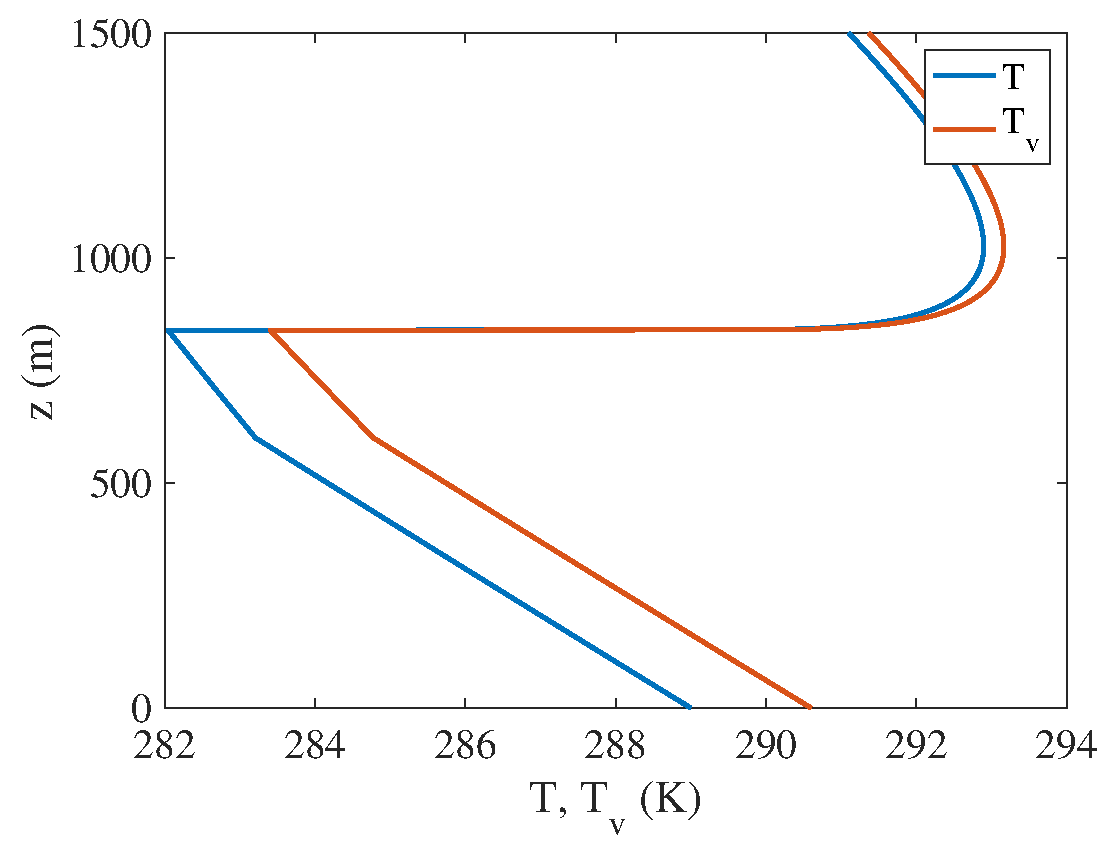
\includegraphics[width=0.49\textwidth]{figures/benchmarks/dycoms/dy_tempe.eps}
	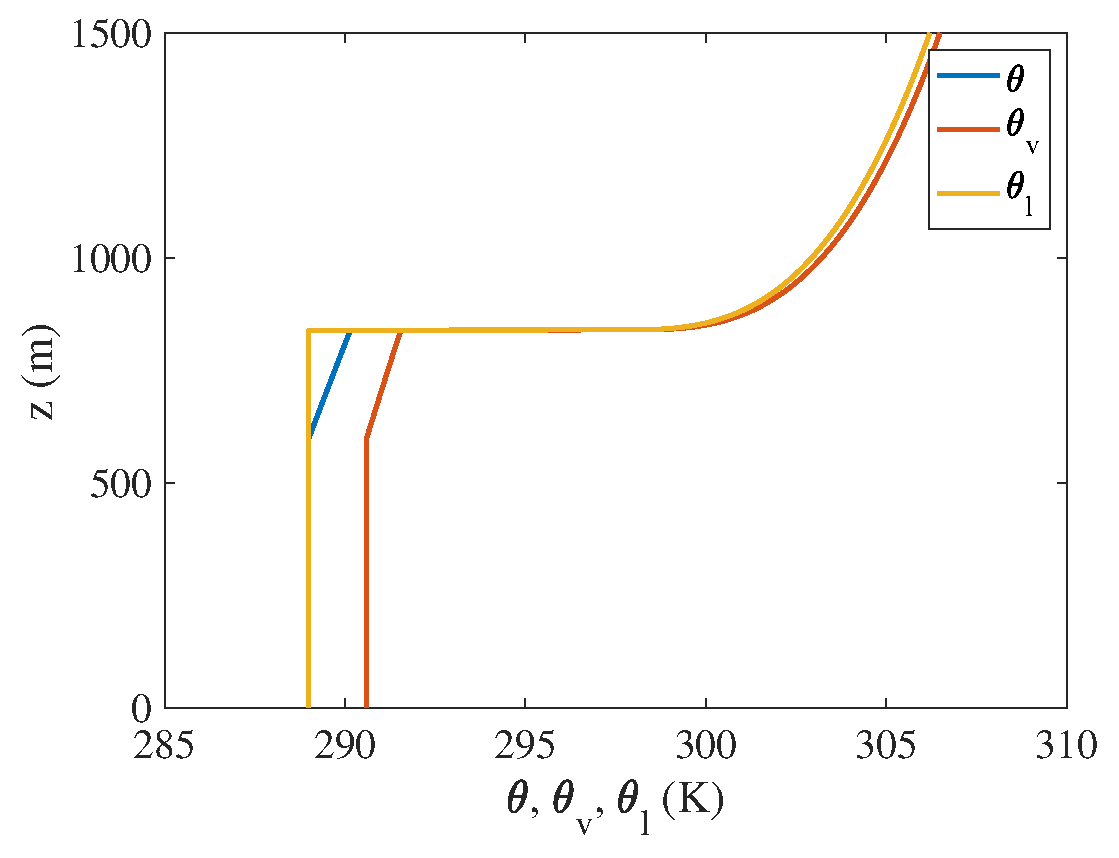
\includegraphics[width=0.49\textwidth]{figures/benchmarks/dycoms/dy_pot_temp.eps}
	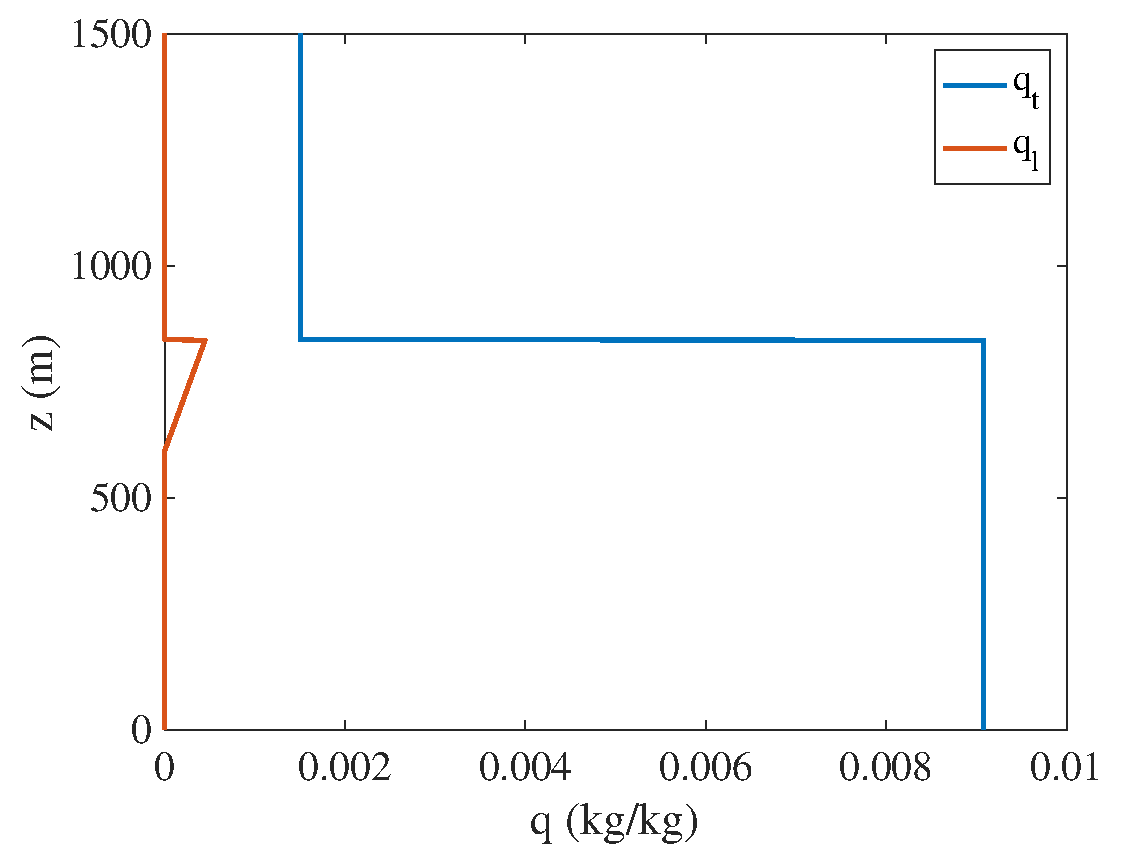
\includegraphics[width=0.49\textwidth]{figures/benchmarks/dycoms/dy_mixing_ratios.eps}
	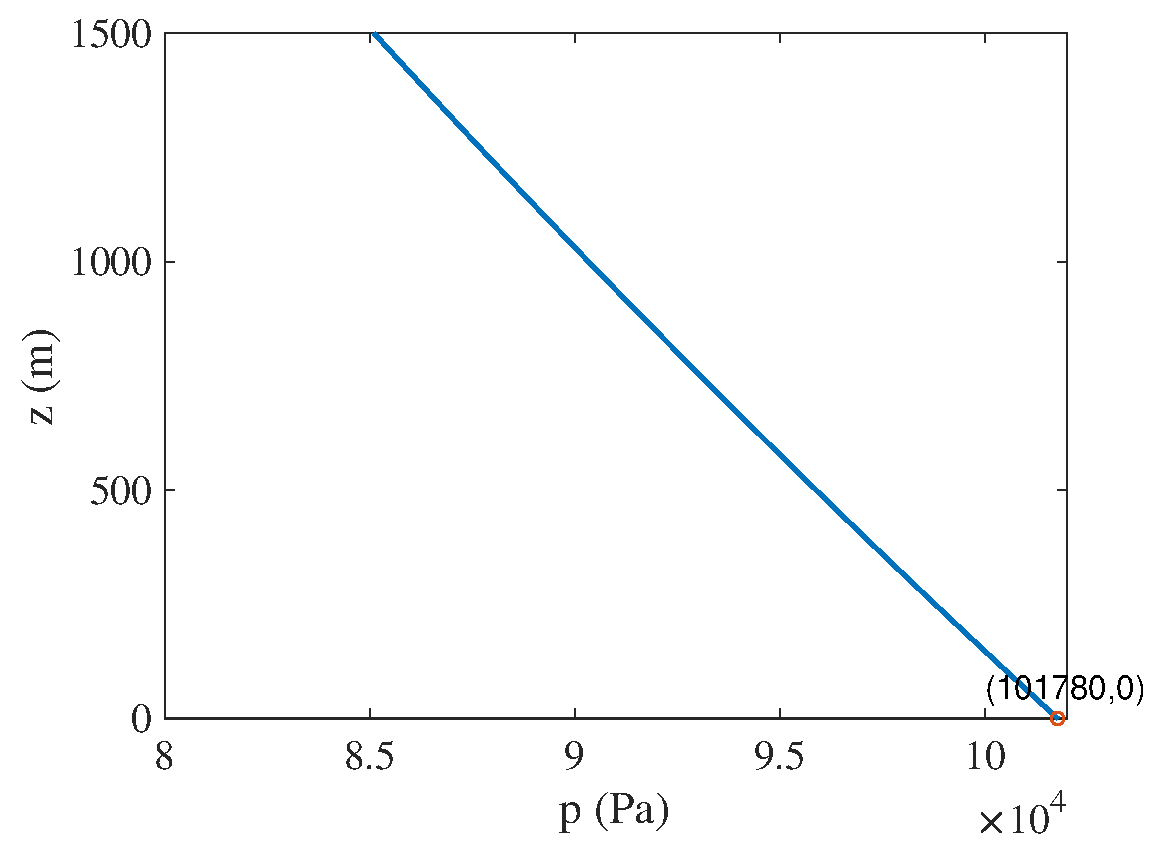
\includegraphics[width=0.49\textwidth]{figures/benchmarks/dycoms/dy_press.eps}
	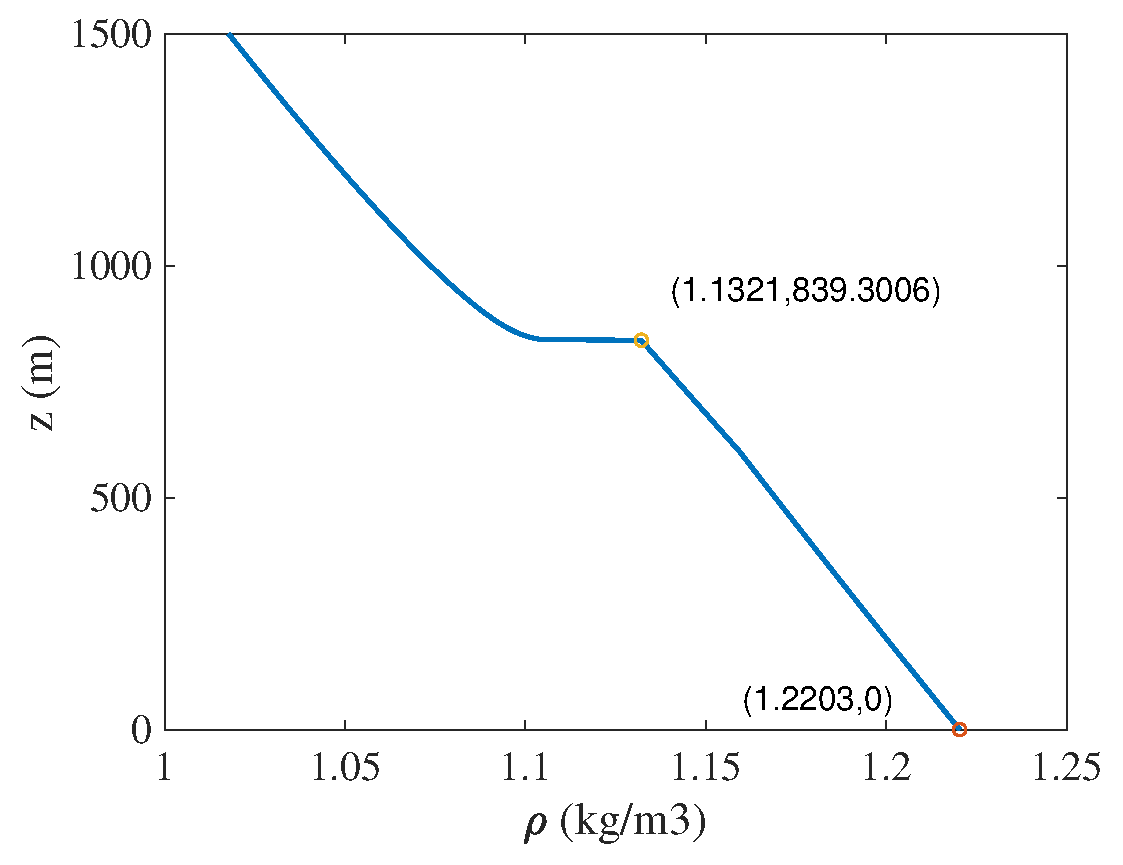
\includegraphics[width=0.49\textwidth]{figures/benchmarks/dycoms/dy_densi.eps}
	%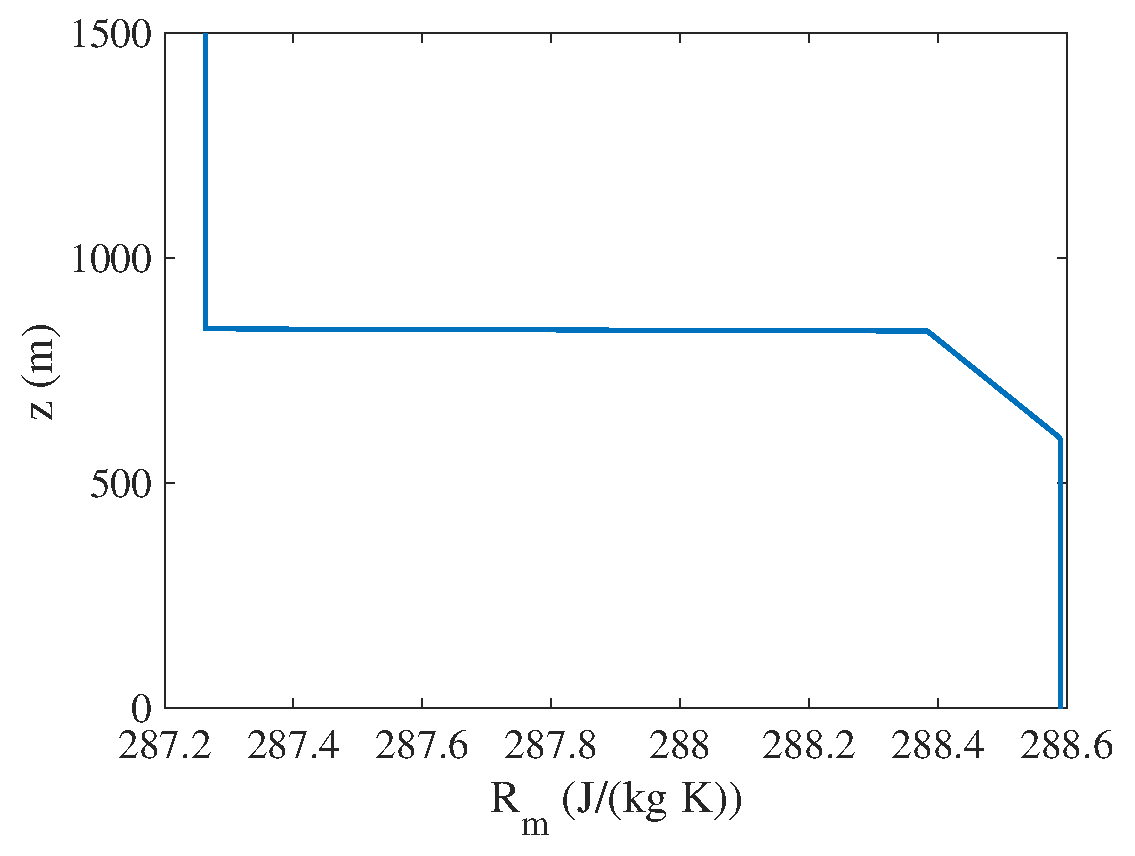
\includegraphics[width=0.49\textwidth]{figures/dy_Rm.eps}
	%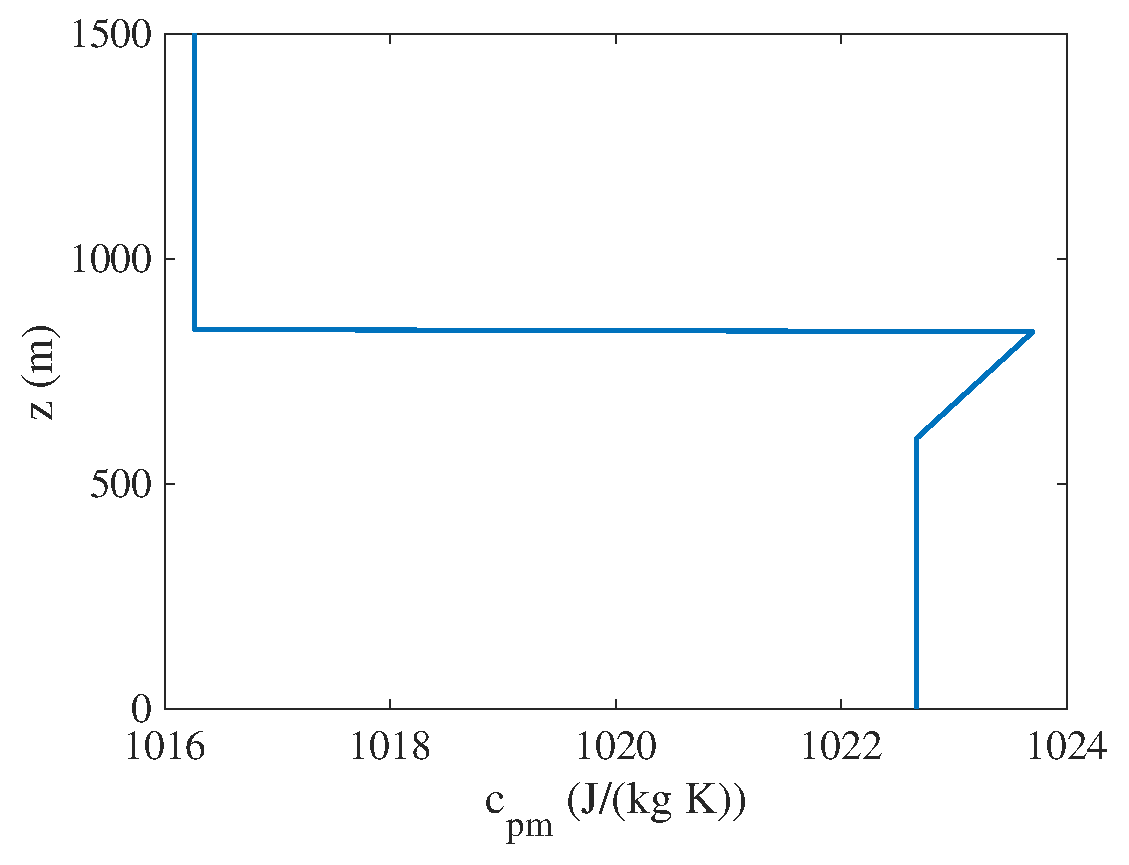
\includegraphics[width=0.49\textwidth]{figures/dy_cpm.eps}
      \caption{DYCOMS: initial states of $T, T_v, \theta, \theta_v, \theta_l, q_t, q_l, p, \rho$.}
\label{dycomsInitFig}
\end{figure}

\subsection{Boundary Conditions}

The bottom boundary conditions for DYCOMS are prescribed energy and water fluxes and a drag law for momentum, as described in section~\ref{s:bottom_bc}. The prescribed fluxes at the surfaces are
\begin{itemize} 
\item Sensible heat flux $\mathrm{SHF} = \vec{\hat n} \cdot (\rho \vec{J}_{\mathrm{sfc}}) = 15\,\mathrm{W~m{^{-2}}}$
\item Latent heat flux $\mathrm{LHF} = \vec{\hat n} \cdot (\rho \vec{D}_{\mathrm{sfc}}) = 115\,\mathrm{W~m^{-2}}$
\item Energy flux $\vec{\hat n} \cdot \rho (\vec{J}_{\mathrm{sfc}} + \vec{D}_{\mathrm{sfc}}) = \mathrm{SHF + LHF} = 130\,\mathrm{W~m^{-2}}$
\item Evaporation $E = \mathrm{LHF}/L_{v}(T_\mathrm{sfc})$ \hl{[Would be good to update code here to use $L_v$ evaluated at surface temperature (but makes little difference).]}
\item \hl{[add surface drag]}
\end{itemize}

\subsection{Sources}

\subsubsection{Radiative cooling}
Radiative cooling is imposed through the simple model described by \cite{Stevens05a}. It specifies the vertical radiative energy flux $\Frad = F_R \vec{\hat k}$ (part of the non-diffusive energy fluxes \eqref{e:ndf_flux}) as
\begin{equation}
    \label{e:radiativeStevens05}
    F_{R}({\bf x}, t) = F_0{\rm e}^{-Q(z,\infty)} +
    F_1{\rm e}^{-Q(0, z)} +
    \rho_i c_{pd} D \alpha_z\frac{(z-z_i)^{4/3}}{4} + z_i(z - z_i)^{1/3}
\end{equation}
where 
\begin{equation}
    Q(a,b) = \kappa\int_{a}^{b}\rho\,q_l\,dz.
\end{equation}
The following parameters are used:
$F_0=70\,\mathrm{W\,m^{-2}}$, $F_1=22\,\mathrm{W\,m^{-2}}$, $\kappa=85\,\mathrm{m^2\,kg^{-1}}$, $\alpha_z=1\,\mathrm{m^{-4/3}}$. The parameter $D=3.75\times 10^{-6}\,\mathrm{s^{-1}}$ gives the large-scale divergence, which also enters the dynamical equations as an additional advection term.  

\subsubsection{Large-scale subsidence}

A large-scale subsidence velocity $W=-Dz$ (positive upward) is imposed and gives rise to a source
\[
-\rho W \vec{\hat k} \cdot \nabla h^\mathrm{tot}
\]
in the energy equation (with total enthalpy $h^\mathrm{tot}$) and a source
\[
-\rho W \vec{\hat k} \cdot \nabla q_t
\]
in the total water specific humidity equation.

\subsubsection{Coriolis forcing}

The geostrophic wind is prescribed following \cite{Stevens05a} as $u_g = 7.0~\mathrm{m~s^{-1}}$ and $v_g = -5.5~\mathrm{m~s^{-1}}$. This gives rise to a source
\[
-\rho f\vec{\hat k} \times (\vec{u}-\vec{u_g})
\]
in the momentum equation, with Coriolis parameter $f = 0.762\times10^{-4}~\mathrm{s^{-1}}$.

\subsection{SGS Fluxes}

The interaction of the resolved flow with SGS fluxes is crucial for a successful simulation of stratocumuli \citep{Pressel17a}. If there is too much spurious mixing across the sharp inversion interface, the clouds dissipate because too much dry air from above the clouds is mixed into the clouds. Hence, it is important to use SGS schemes that limit mixing near the stable inversion interface.

\subsection{Results}
Figures \ref{fig:dycomsWWresultLSRK14-smago} and \ref{fig:dycomsWWresultLSRK14-vreman} show the 4-hr time-averaged vertical moment $<w'w'>$ for the explicit (single-rate) LSRK14 solution using the Smagorinsky-Lilly SGS models and, respectively, the Vreman SGS model. The solution corresponds to a simulation in domain $\Omega=1000\times 1000 \times 2500\,{\rm m^3}$ using the vertical and horizontal resolutions indicated in each figure. 

\begin{figure}
    \centering
	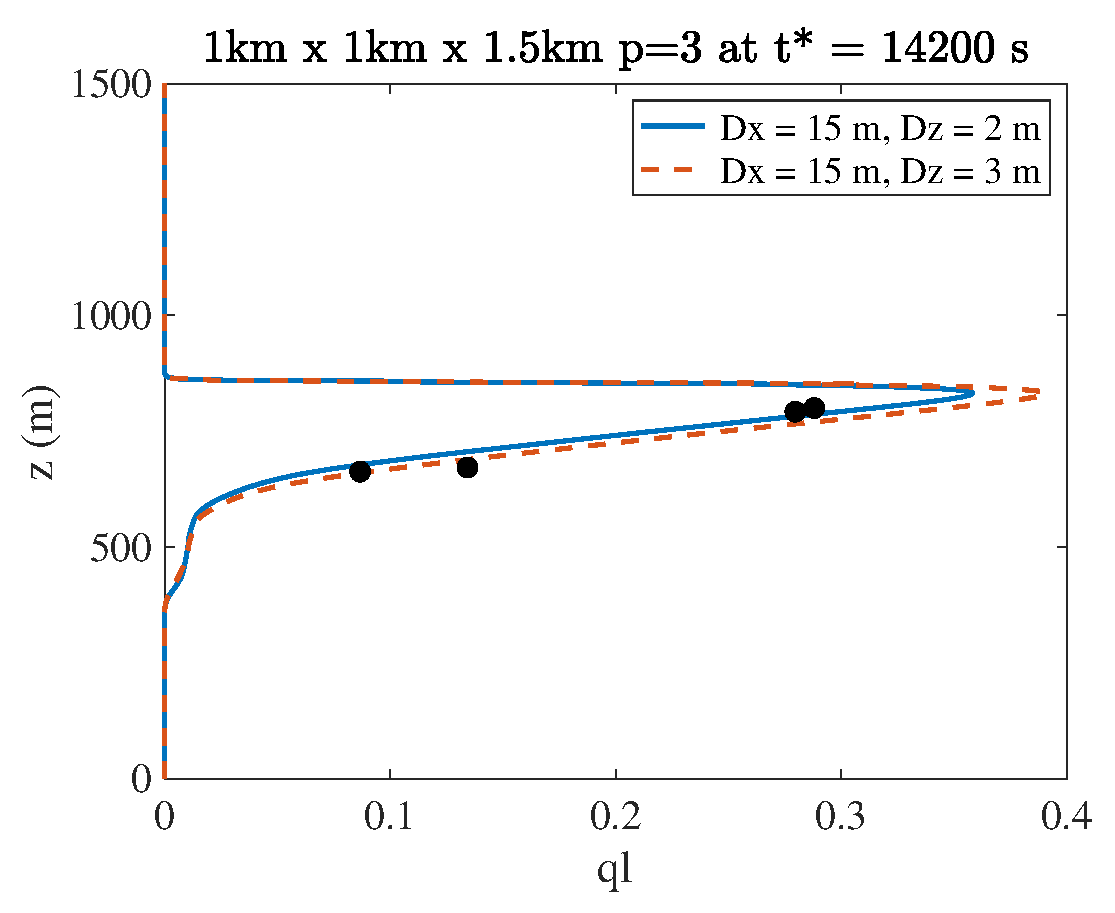
\includegraphics[width=0.3\textwidth]{./figures/benchmarks/dycoms/dycoms_smago_dz_3m_vs_2m_qt9_dycoms_ql_15mX15mX2m_t14200s-legend}
	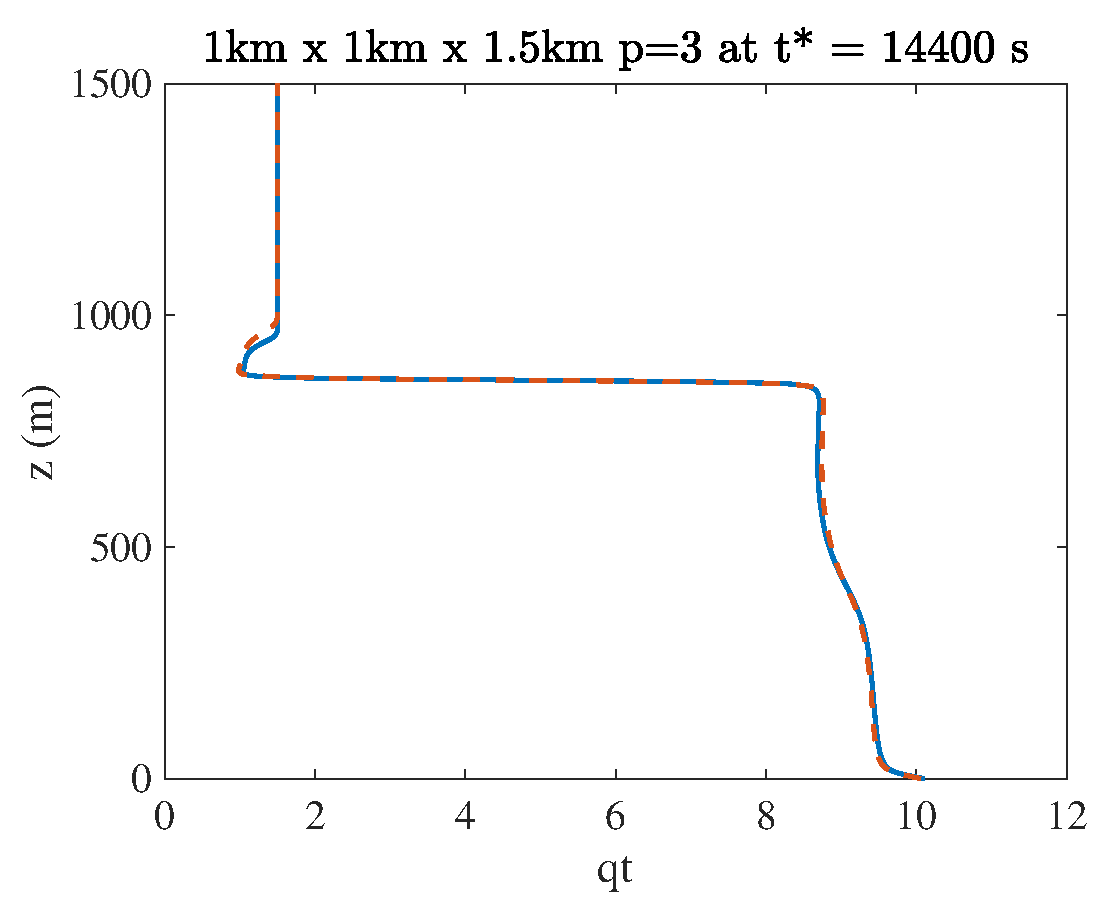
\includegraphics[width=0.3\textwidth]{./figures/benchmarks/dycoms/dycoms_smago_dz_3m_vs_2m_qt9_dycoms_qt_15mX15mX2m_t14400s}
	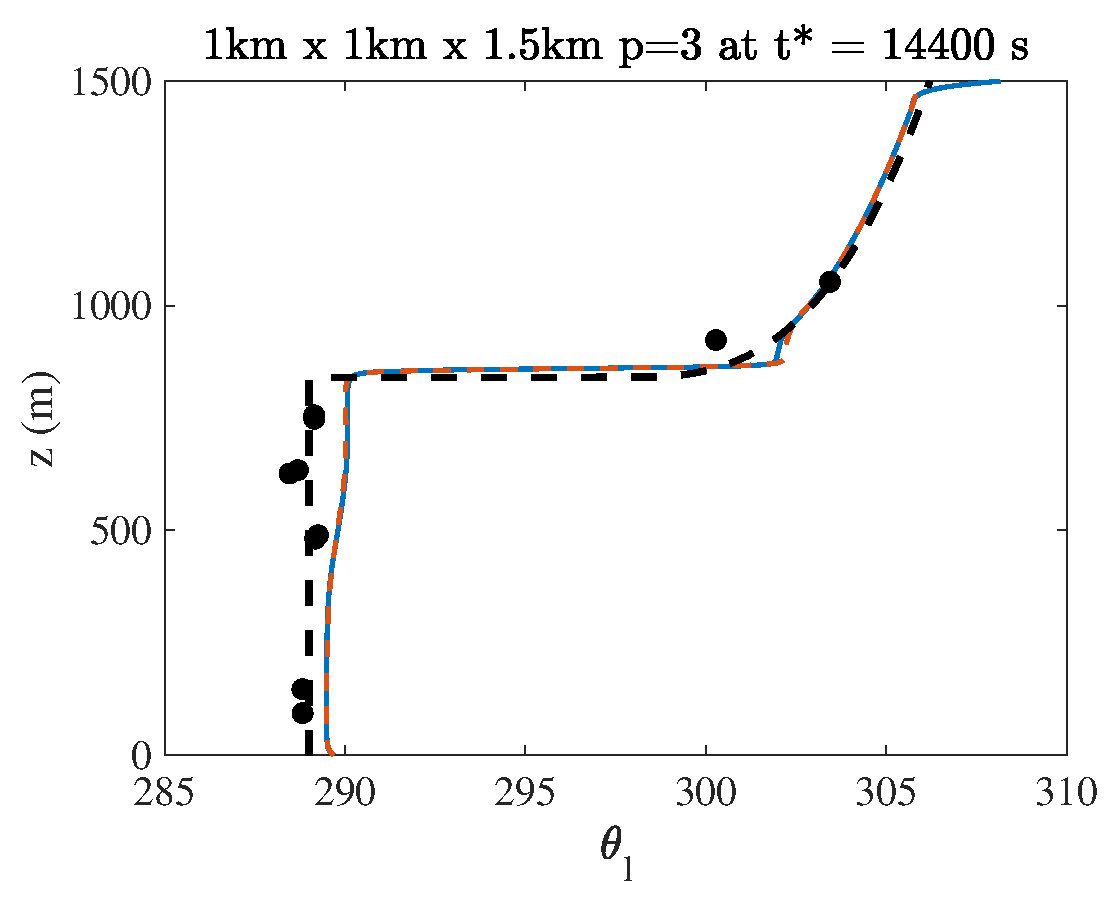
\includegraphics[width=0.3\textwidth]{./figures/benchmarks/dycoms/dycoms_smago_dz_3m_vs_2m_qt9_dycoms_thl_15mX15mX2m_t14400s}
	
	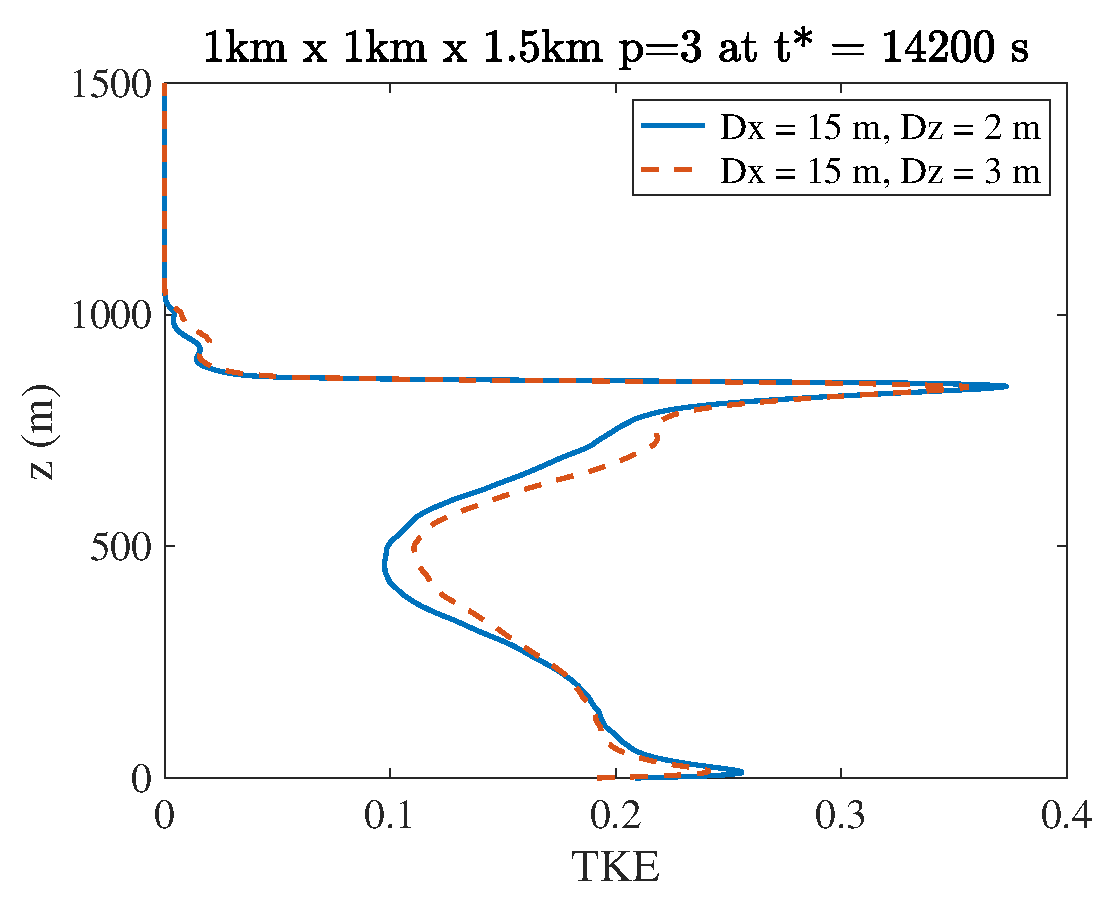
\includegraphics[width=0.3\textwidth]{./figures/benchmarks/dycoms/dycoms_smago_dz_3m_vs_2m_qt9_dycoms_tke_15mX15mX2m_t14200s-legend}
	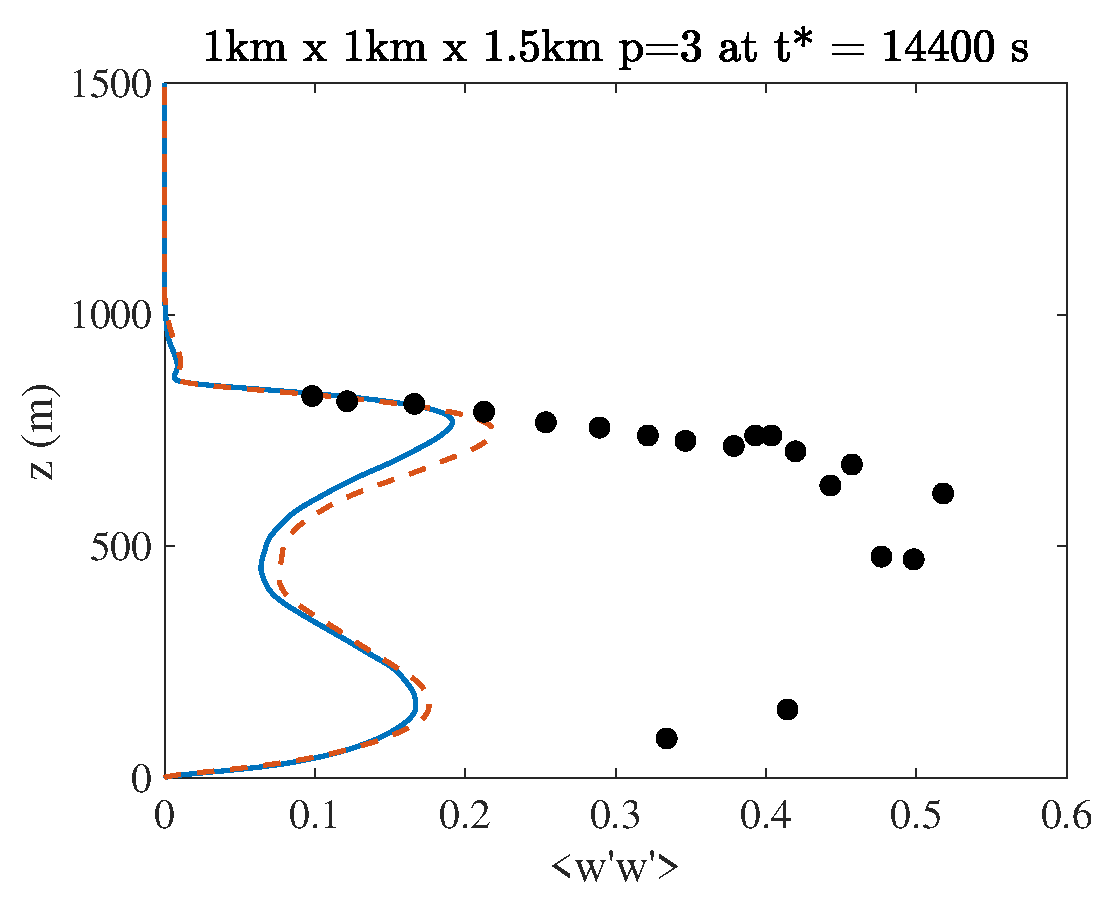
\includegraphics[width=0.3\textwidth]{./figures/benchmarks/dycoms/dycoms_smago_dz_3m_vs_2m_qt9_dycoms_ww_15mX15mX2m_t14400s}
	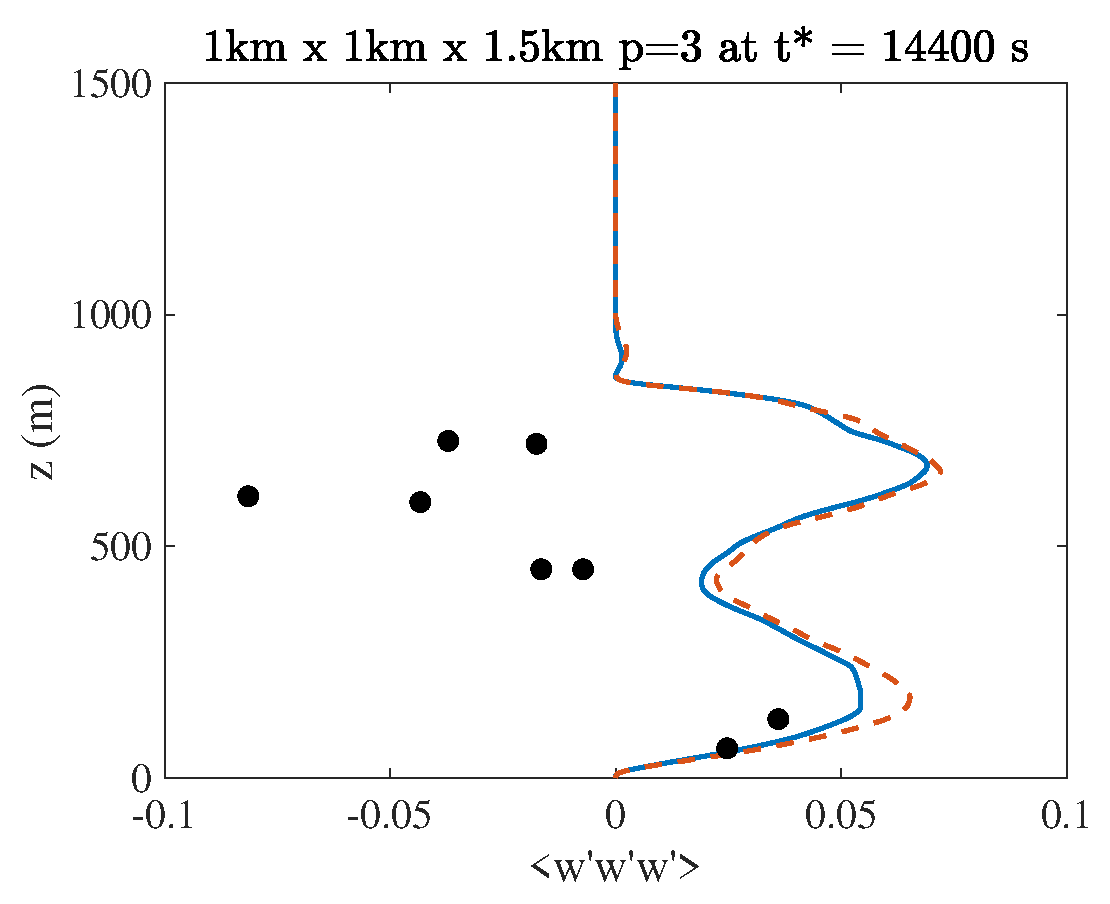
\includegraphics[width=0.3\textwidth]{./figures/benchmarks/dycoms/dycoms_smago_dz_3m_vs_2m_qt9_dycoms_www_15mX15mX2m_t14400s}
	
    \caption{DYCOMS reference solutions with  Smagorinsky-Lilly SGS using effective vertical resolution $\Delta z=2\,{\rm m}$ and $\Delta z=3\,{\rm m}$ and horizontal resolution $\Delta x=\Delta y=15\,{\rm m}$. The black circles indicate the measurements collected during the research flight.}
\label{fig:dycomsWWresultLSRK14-smago}
\end{figure}


\begin{figure}
    \centering
        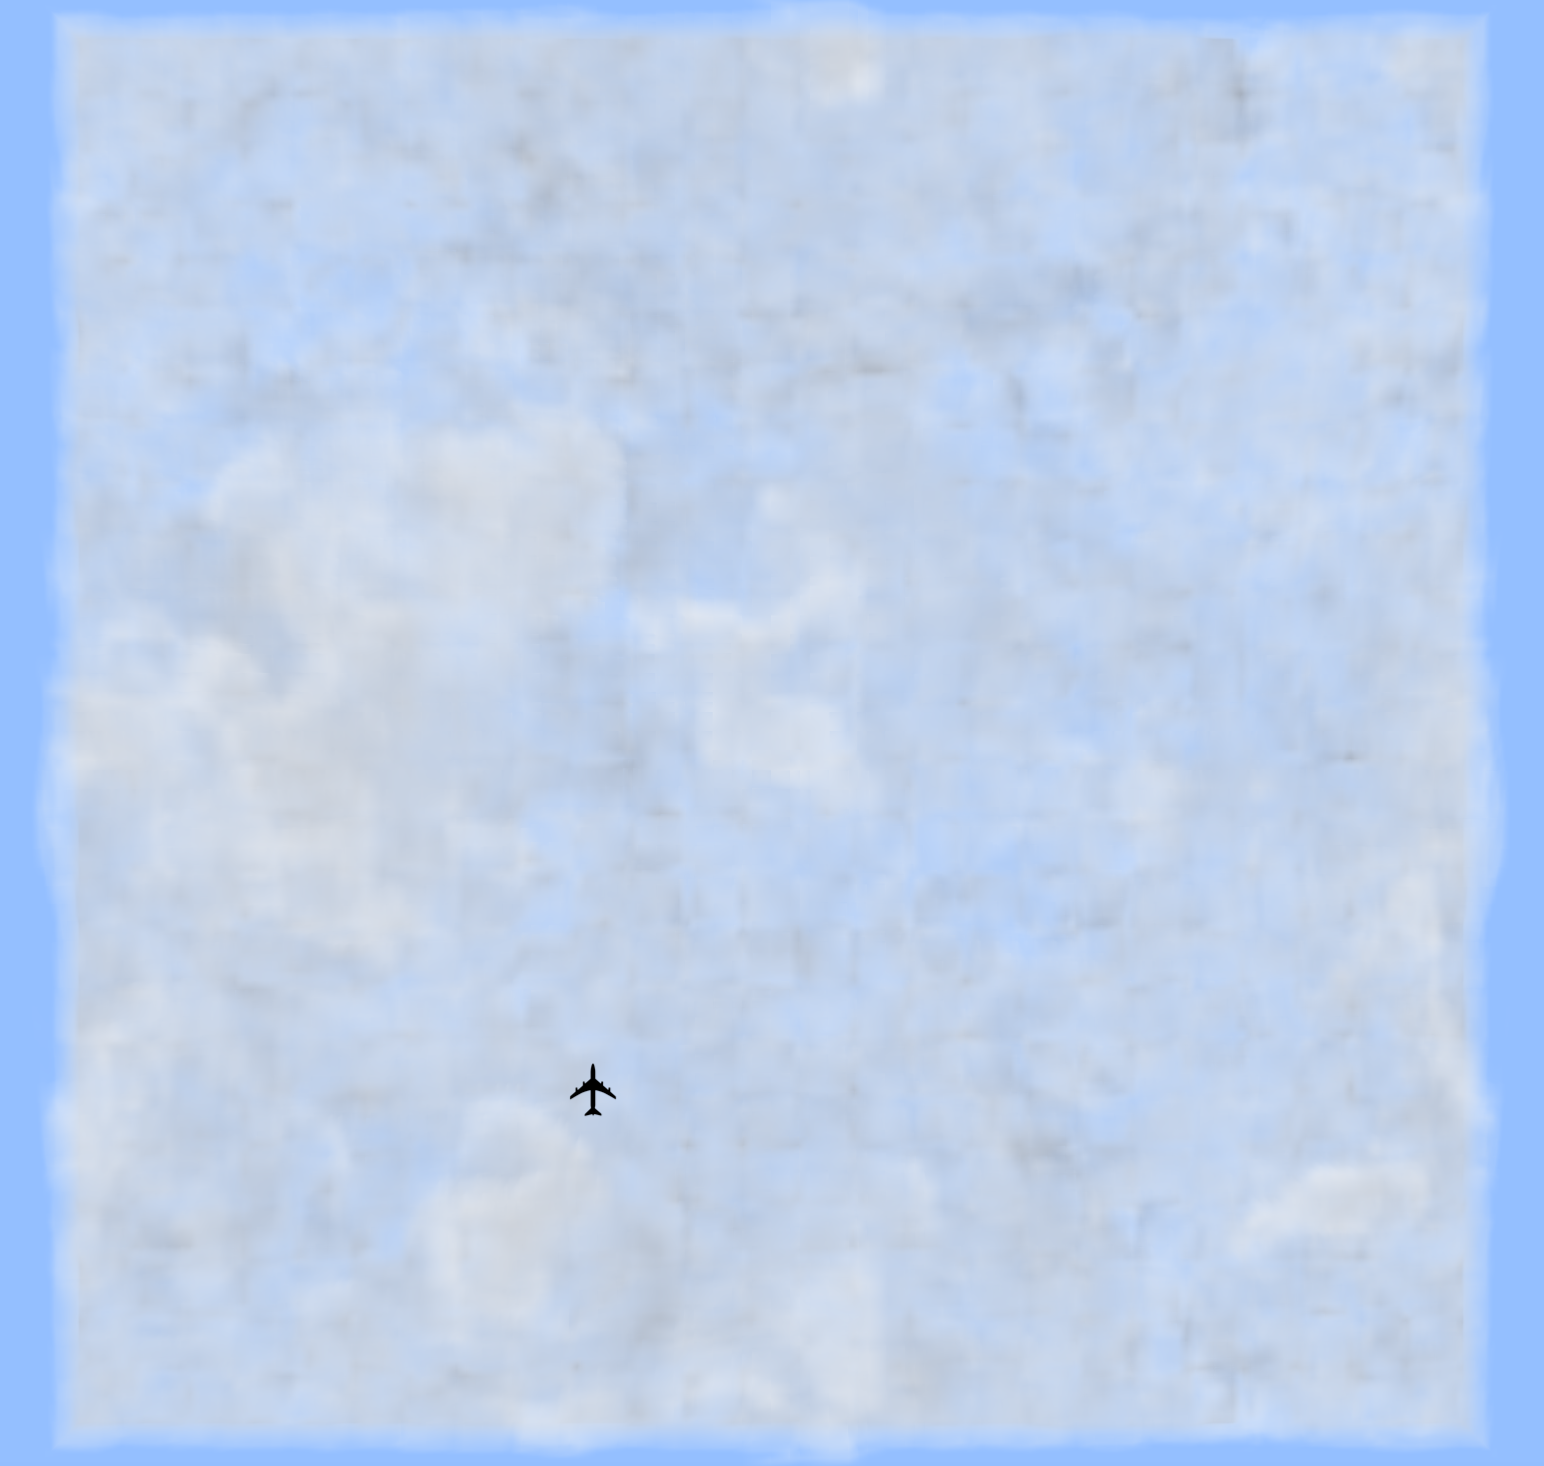
\includegraphics[width=0.5\textwidth]{./figures/benchmarks/dycoms/cloud_b747.png}
		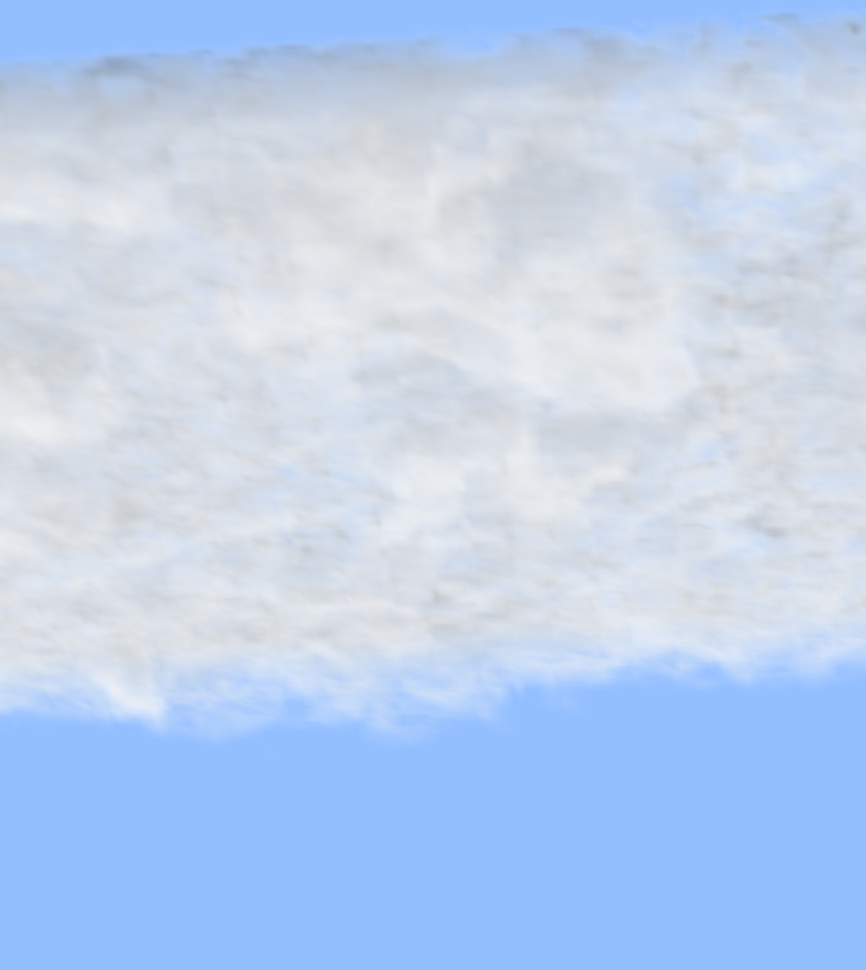
\includegraphics[width=0.425\textwidth]{./figures/benchmarks/dycoms/dycoms-view-below-angle.png}
	\caption{Dycoms: instantaneous volume rendering of $q_l$ at $t=4\,{\rm h}$. Left: planar with a superimposed silhouette of the airplane was for scale. Right: south-view of a cloud section. Domain size: $3 \times 3 \times 1.5\,{\rm km^3}$ and effective resolution $\Delta x = \Delta y = 25\,{\rm m} \times \Delta z = 12\,{\rm m}$. This effective resolution using $4^{th}$-order  yields a smallest nodal distance of $17\,{\rm m}$ and $8\,{\rm m}$ in the horizontal and vertical directions, respectively.  (Airplane silhouette source: clipart-library.com).}
	\label{fig:DYCOMS_ql_rendering}
\end{figure}

\begin{figure}
    \centering
        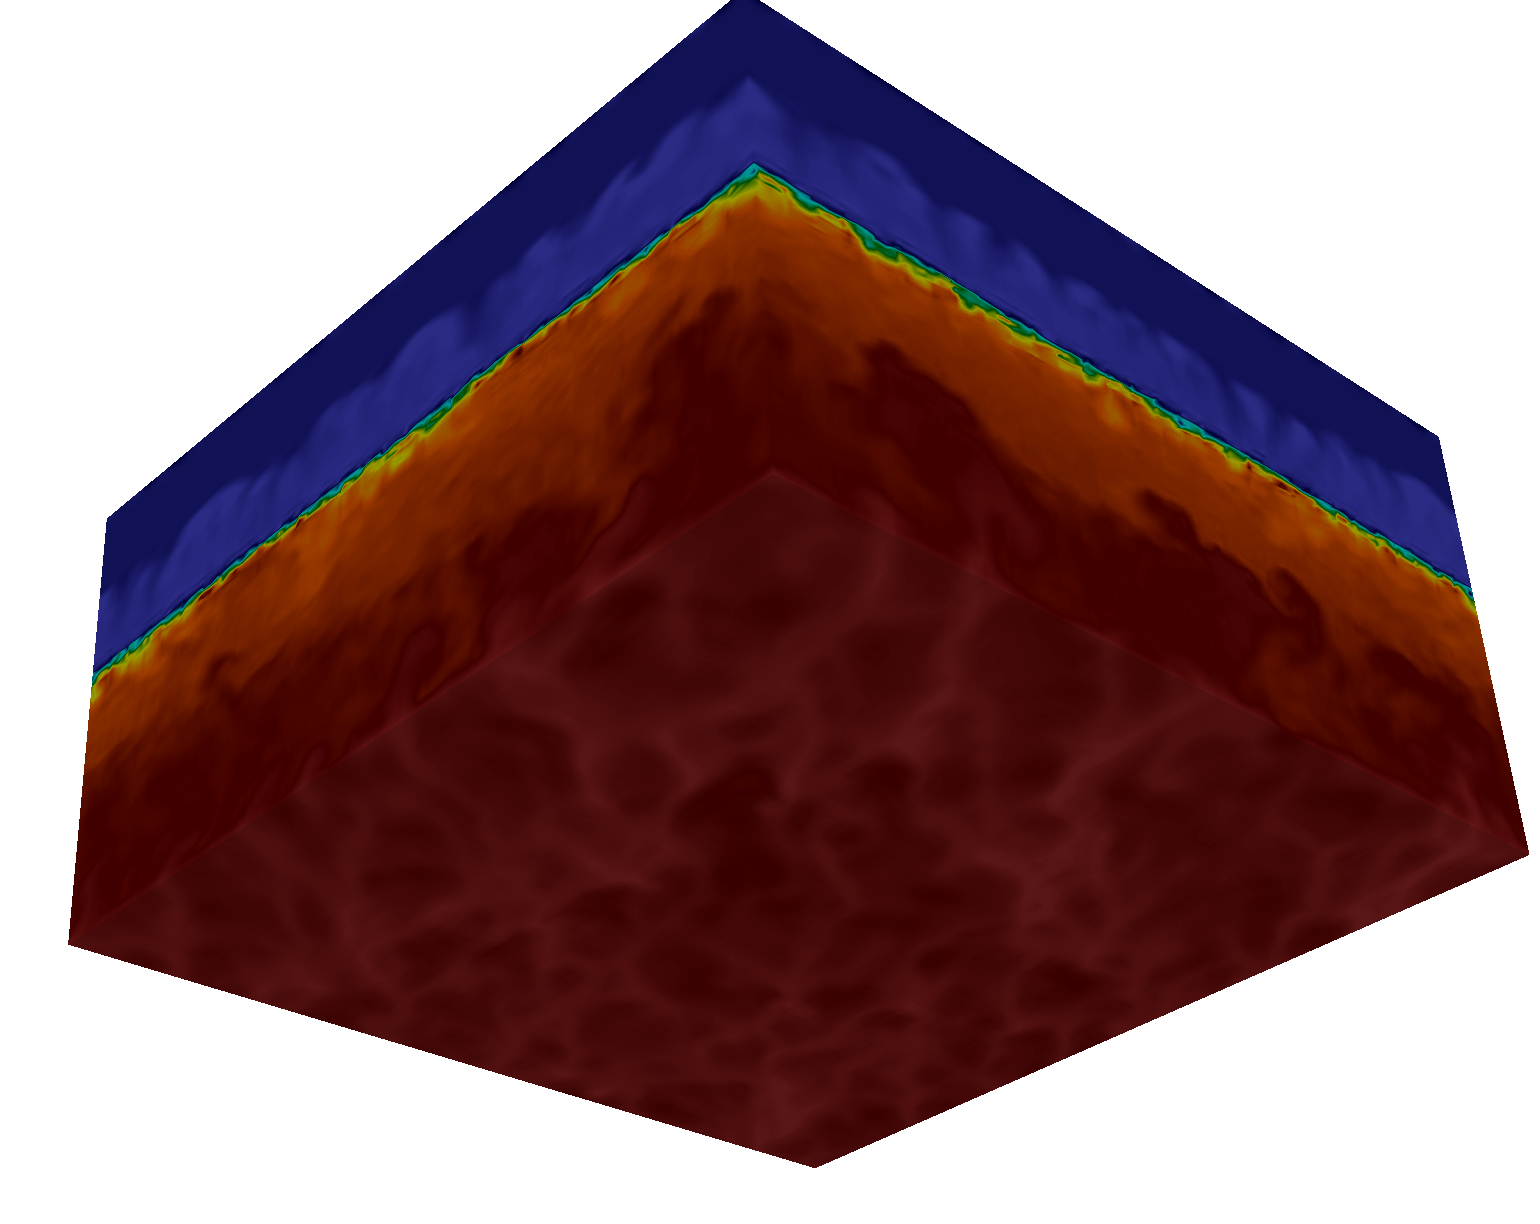
\includegraphics[width=0.9\textwidth]{./figures/benchmarks/dycoms/qtot0060.png}
	\caption{Dycoms: an instantaneous perspective view of $q_t$ during the simulation. Domain size: $3 \times 3 \times 1.5\,{\rm km^3}$ and effective resolution $\Delta x = \Delta y = 25\,{\rm m} \times \Delta z = 12\,{\rm m}$. This effective resolution using $4^{th}$-order  yields a smallest nodal distance of $17\,{\rm m}$ and $8\,{\rm m}$ in the horizontal and vertical directions, respectively. The turbulent structure of the rising plumes of total water is visible. }
	\label{fig:DYCOMS_qt_contours}
\end{figure}

\section{3D Squall Line}
\label{sq3D}
The three-dimensional simulation of a squall line is defined in a domain
$60\times 60\times24\,\mathrm{km}^3$. 

\paragraph{Boundary conditions}
\begin{itemize}
\item Bottom:
    \begin{itemize}
        \item Momentum: free slip b.c. ${\bf u}\cdot{\bf u}= 0$
        \item \hl{[Energy: nothing as of now. But we need to apply no thermal flux by imposing Neumann on $\nabla T$]}.
    \end{itemize}
\item Top: thick sponge (almost 1/3 of the vertical domain.)
\item Lateral: periodic in both horizontal directions.
\end{itemize}

\paragraph{Grid resolution} For testing purposes only, a relatively coarse resolution is the default setting with $(\Delta {\rm horizontal}\times \Delta {\rm vertical}) = (250\,{\rm m}, \times 100\,{\rm m})$. To decrease the number of vertical layers, a stretched grid along $z$ can be used to make the resolution higher in the lower atmosphere where convection is triggered. 

\paragraph{Physical phenomenon}
The domain is crossed by a horizontal wind along the x-direction with a $12\,\mathrm{m\,s^{-1}}$ shear at $z=2000\,\mathrm{m}$.
The initial background state is given by the sounding of \cite{gabersekGiraldoDoyle2012}.
To initiate the vertical transport of water vapor to a level of condensation (and hence trigger a cloud formation, the initial background is forced by a temperature anomaly $\theta'$ $3$ K warmer than the surrounding environment. The cloud first forms at approximately 500 s, and is fully develop after 4500 s. 

An instantaneous view of the precipitating squall line is shown in Figure \ref{fig:benchmarks/squall1}. 

\begin{figure}[htbp]
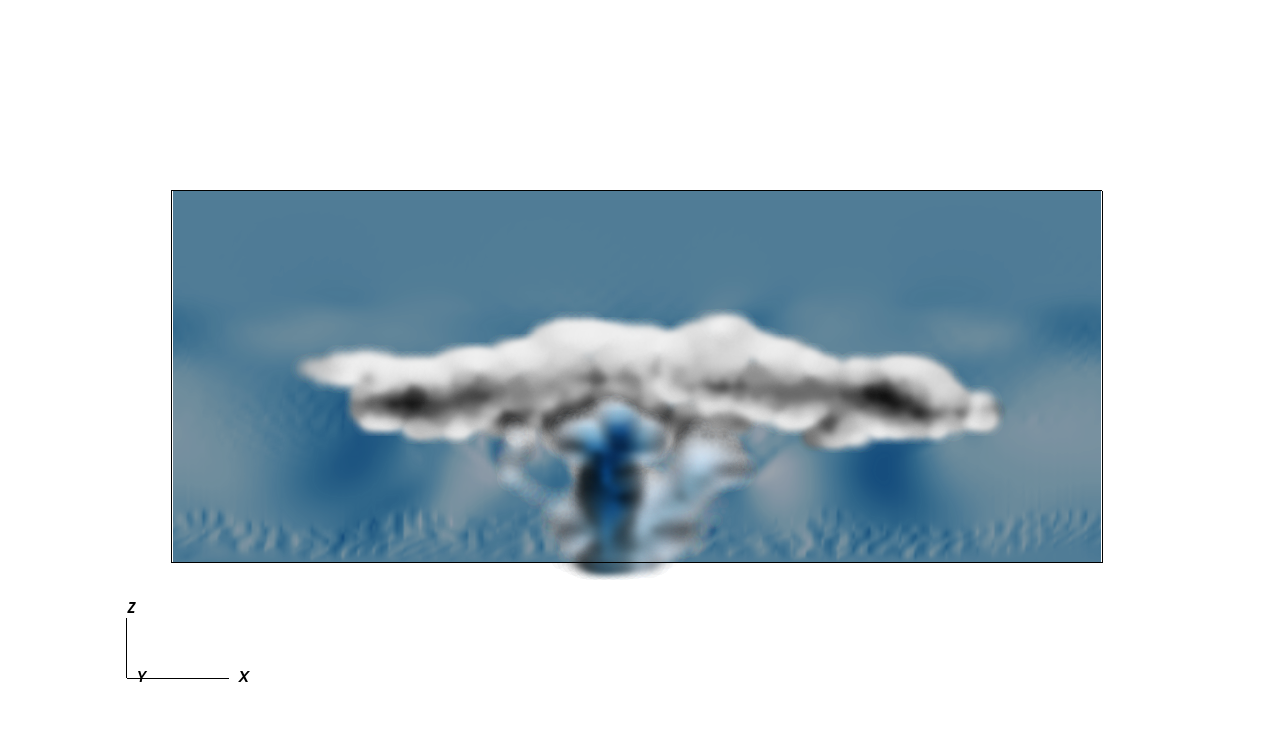
\includegraphics[width=1.2\textwidth]{figures/squall_working_warm_rain_frontal_view0028.png}
\caption{Front view of a fully developed squall line with precipitating rain. }
\label{fig:benchmarks/squall1}
\end{figure}

\section{External Soundings}
External soundings can be read into the code for initialization purposes. The sounding requires the format reported in Table \ref{tab:DeltaDefinitionsTable}.

\begin{table*}[t]
\centering
{\footnotesize
\caption[short]{Structure of sounding files for simulation initialization.}
\label{tab:DeltaDefinitionsTable}
\begin{tabular*}{\textwidth}{ @{\extracolsep{\fill}} llllll}
\hline
\hline
z (m) & $\theta_v$ (K) & $q_{tot}$ $\rm {kg/kg}$ & $u$ (m/s) & $v$ (m/s) & p (Pa)\\
0 & 300 & 14  & -2 & 0 & 100000\\
... & ... & ...  & ... & ... & ...\\
\hline
\hline
\end{tabular*}
}
\end{table*}

\chapter{Input/Output}

\hl{[TS: We need software design document, and I'd move this there.]}

\section{Inputs}

\section{Outputs}
\section{Three dimensional fields}


\section{Diagnostics}

A Reynolds decomposition is applied to all quantities for which statistics are computed. For a given quantity $a$, it is split into a mean value, $\langle a \rangle$  (in either time or space) and a fluctuation, $a'$, around it such that $a' = a - \langle a \rangle$, where the space or time averaging is simply:

\begin{equation}
    \langle a \rangle = \frac{1}{N} \sum_{i=1}^N a_i
\end{equation}
where $N$ indicates either the number of time or space samples. \hl{An ensemble average should also be added at some point}.

For space averaging, data are first interpolated onto an auxiliary Cartesian mesh with equally spaced nodes. The auxiliary mesh is usually coarser than the solution mesh.
The spatial means are computed across two-dimensional slices of the auxiliary mesh at each vertical level  \hl{to be done}.

The statistics listed in Table \ref{tab:stats} are calculated during the simulation at a regular interval defined by the user. 

\begin{table*}[t]
\centering
{\footnotesize
\caption[short]{Structure of sounding files for simulation initialization.}
\label{tab:stats}
\begin{tabular*}{\textwidth}{ @{\extracolsep{\fill}} lccc}
\hline
\hline
Vertical velocity variance & & &$<w' w'>$\\
Third moment of vertical velocity & & &$<w'w'w'>$\\
Vertical heat flux & & &$<w' \theta'>$\\
Vertical water vapor flux & & &$<w' q_v'>$\\
...\\
\hline
\hline
\end{tabular*}
}
\end{table*}

The velocity two-point correlation is used to extract the energy spectrum as follows:

\begin{equation}
    E(k) = \int \Phi_{ij}dV
\end{equation}

The energy spectrum is calculated by means of the i of the velocity spectrum The velocity spectrum is first calculated by means of the Fourier transform of the correlation 

\section{File formats}
Three dimensional data are written to disk in parallel (one file per processor \hl{Jeremy, please confirm}) using the {\it Visualization Toolkit} (VTK) format (\cite{vtkWeb}). The user defines the writing interval.
VTK should soon be replaced by the HDF5 file format (\cite{hdf5web}).
Statistical quantities are now written out to ASCII files which are read and plotted via a set of Python scripts (under construction).


%-------Bibliography
\bibliographystyle{agufull08}
\bibliography{Giraldo_refs,CLIMA-refs}

\end{document}

% Previous reference state definition

It helps here to distinguish the cases of an isothermal atmosphere and of an atmosphere with nonzero lapse rate:
\begin{itemize}

\item \textbf{Nonzero Lapse Rate ($\Gamma \ge 0$, $T_{v, \mathrm{sfc}} \ge T_{\min}$).}
Integrating the general expression \eqref{e:hydro_pressure} for the hydrostatic pressure for a temperature profile \eqref{e:ref_temperature} with nonzero lapse rate yields
\begin{equation}\label{e:hydro_pressure_lapse}
p_r(z) = p_{\mathrm{MSLP}} \times
\begin{cases}
\left(1 - \frac{\Gamma z}{T_{v, \mathrm{sfc}}} \right)^{g/(R_d \Gamma)} & \text{for } z \le z_t, \\[1.5ex]
  \left(\frac{T_{\min}}{T_{v, \mathrm{sfc}}} \right)^{g/(R_d \Gamma)}
 \exp  \left(-\frac{z - z_t}{H_{\min}} \right) & \text{for } z\ge z_t, 
\end{cases}
\end{equation}
where 
\begin{equation}
H_{\min} = \frac{R_d T_{\min}}{g}
\end{equation}
is the ``stratospheric'' scale height. See See Fig.~\ref{f:hydrostatic_state}b (red line) for an example. (The expression \eqref{e:hydro_pressure_lapse} for nonzero lapse rate converges to the expression \eqref{e:hydro_pressure_iso} for zero lapse rate in the limit $\Gamma \to 0$, as can be verified by L'H{\^o}pital's rule.)
\end{itemize}
